%%%%%%%%%%%%%%%%%%%%%%%%%%%%%%%%%%%%%%%%%
% Florida Institute of Technology 
% OCE4531 - Instrumentation Design and Measurement 
% Lecture Notes
%
% Authors:
% Braidan Duffy
%
% Developed using the kaobook LaTeX Template
% Version 1.3 (December 9, 2021)
% For the latest template development version and to make contributions:
% https://github.com/fmarotta/kaobook
%
%%%%%%%%%%%%%%%%%%%%%%%%%%%%%%%%%%%%%%%%%

%----------------------------------------------------------------------------------------
%	PACKAGES AND OTHER DOCUMENT CONFIGURATIONS
%----------------------------------------------------------------------------------------

\documentclass[
	letterpaper, % Page size
	fontsize=10pt, % Base font size
	twoside=true, % Use different layouts for even and odd pages (in particular, if twoside=true, the margin column will be always on the outside)
	%open=any, % If twoside=true, uncomment this to force new chapters to start on any page, not only on right (odd) pages
	%chapterentrydots=true, % Uncomment to output dots from the chapter name to the page number in the table of contents
	numbers=noenddot, % Comment to output dots after chapter numbers; the most common values for this option are: enddot, noenddot and auto (see the KOMAScript documentation for an in-depth explanation)
]{kaobook}

% Choose the language
\ifxetexorluatex
	\usepackage{polyglossia}
	\setmainlanguage{english}
\else
	\usepackage[english]{babel} % Load characters and hyphenation
\fi
\usepackage[english=british]{csquotes}	% English quotes

\usepackage[]{outlines}

\usepackage{color, soul} % Enable text color changes and highlighting

\usepackage{cancel}

\usepackage[]{pdfpages}

\usepackage{diagbox}

\usepackage{karnaugh-map}

% Load packages for testing
% \usepackage{blindtext}
%\usepackage{showframe} % Uncomment to show boxes around the text area, margin, header and footer
%\usepackage{showlabels} % Uncomment to output the content of \label commands to the document where they are used

% Load the bibliography package
\usepackage{kaobiblio}
% \addbibresource{bibliographies/learning_materials.bib} % Learning Materials bibliography file
% \addbibresource{bibliographies/main.bib} % Bibliography file

% Load mathematical packages for theorems and related environments
\usepackage[framed=true]{kaotheorems}

% Load the package for hyperreferences
\usepackage{kaorefs}

\graphicspath{{images/}} % Paths in which to look for images

\makeindex[columns=3, title=Alphabetical Index, intoc] % Make LaTeX produce the files required to compile the index

\makeglossaries % Make LaTeX produce the files required to compile the glossary
\newglossaryentry{computer}{
	name=computer,
	description={is a programmable machine that receives input, stores and manipulates data, and provides output in a useful format}
}

% Glossary entries (used in text with e.g. \acrfull{fpsLabel} or \acrshort{fpsLabel})
\newacronym[longplural={Frames per Second}]{fpsLabel}{FPS}{Frame per Second}
\newacronym[longplural={Tables of Contents}]{tocLabel}{TOC}{Table of Contents}

 % Include the glossary definitions

\makenomenclature % Make LaTeX produce the files required to compile the nomenclature

% Reset sidenote counter at chapters
%\counterwithin*{sidenote}{chapter}

\usepackage{xcolor}
\definecolor{codegreen}{rgb}{0,0.6,0}
\definecolor{codegray}{rgb}{0.5,0.5,0.5}
\definecolor{codepurple}{rgb}{0.58,0,0.82}
\definecolor{backcolour}{rgb}{0.95,0.95,0.92}
\lstdefinestyle{mystyle}{
    backgroundcolor=\color{backcolour},   
    commentstyle=\color{codegreen},
    keywordstyle=\color{blue},
    numberstyle=\tiny\color{codegray},
    stringstyle=\color{codepurple},
    basicstyle=\ttfamily\footnotesize,
    breakatwhitespace=false,         
    breaklines=true,                 
    captionpos=b,                    
    keepspaces=true,                 
    numbers=left,                    
    numbersep=5pt,                  
    showspaces=false,                
    showstringspaces=false,
    showtabs=false,                  
    tabsize=2
}
\lstset{style=mystyle}

%----------------------------------------------------------------------------------------

\begin{document}

%----------------------------------------------------------------------------------------
%	BOOK INFORMATION
%----------------------------------------------------------------------------------------

\titlehead{OCE4531 Lecture Notes}
\subject{Florida Institute of Technology: OCE4531}

\title{Instrumentation Design and Measurement Analysis}
\subtitle{A Compendium of Knowledge}

\author{Braidan Duffy}

\date{May 5, 2022}

\publishers{Florida Institute of Technology}

%----------------------------------------------------------------------------------------

\frontmatter % Denotes the start of the pre-document content, uses roman numerals

%----------------------------------------------------------------------------------------
%	OPENING PAGE
%----------------------------------------------------------------------------------------

%\makeatletter
%\extratitle{
%	% In the title page, the title is vspaced by 9.5\baselineskip
%	\vspace*{9\baselineskip}
%	\vspace*{\parskip}
%	\begin{center}
%		% In the title page, \huge is set after the komafont for title
%		\usekomafont{title}\huge\@title
%	\end{center}
%}
%\makeatother

%----------------------------------------------------------------------------------------
%	COPYRIGHT PAGE
%----------------------------------------------------------------------------------------

\makeatletter
\uppertitleback{\@titlehead} % Header

\lowertitleback{
	\textbf{Disclaimer}\\
	You can edit this page to suit your needs. For instance, here we have a no copyright statement, a colophon and some other information. This page is based on the corresponding page of Ken Arroyo Ohori's thesis, with minimal changes.
	
	\medskip
	
	\textbf{License}\\
	Copyright 2022 \@author\\

	Permission is hereby granted, free of charge, to any person obtaining a copy of this software and associated documentation files (the “Software”), to deal in the Software without restriction, including without limitation the rights to use, copy, modify, merge, publish, distribute, sublicense, and/or sell copies of the Software, and to permit persons to whom the Software is furnished to do so, subject to the following conditions:

	The above copyright notice and this permission notice shall be included in all copies or substantial portions of the Software.

	THE SOFTWARE IS PROVIDED “AS IS”, WITHOUT WARRANTY OF ANY KIND, EXPRESS OR IMPLIED, INCLUDING BUT NOT LIMITED TO THE WARRANTIES OF MERCHANTABILITY, FITNESS FOR A PARTICULAR PURPOSE AND NONINFRINGEMENT. IN NO EVENT SHALL THE AUTHORS OR COPYRIGHT HOLDERS BE LIABLE FOR ANY CLAIM, DAMAGES OR OTHER LIABILITY, WHETHER IN AN ACTION OF CONTRACT, TORT OR OTHERWISE, ARISING FROM, OUT OF OR IN CONNECTION WITH THE SOFTWARE OR THE USE OR OTHER DEALINGS IN THE SOFTWARE.
	
	\medskip
	
	\textbf{Colophon} \\
	This document was typeset with the help of \href{https://sourceforge.net/projects/koma-script/}{\KOMAScript} and \href{https://www.latex-project.org/}{\LaTeX} using the \href{https://github.com/fmarotta/kaobook/}{kaobook} class.
	
	The source code of this book is available at:\\\url{https://github.com/fmarotta/kaobook}
	
	(You are welcome to contribute!)
	
	\medskip
	
	\textbf{Publisher} \\
	First printed in May 2022 by \@publishers
}
\makeatother

%----------------------------------------------------------------------------------------
%	DEDICATION
%----------------------------------------------------------------------------------------

\dedication{
	\emph{Ab Experentia, Illustratio}
}

%----------------------------------------------------------------------------------------
%	OUTPUT TITLE PAGE AND PREVIOUS
%----------------------------------------------------------------------------------------

% Note that \maketitle outputs the pages before here

\maketitle

%----------------------------------------------------------------------------------------
%	PREFACE
%----------------------------------------------------------------------------------------

\chapter*{Preface}
\addcontentsline{toc}{chapter}{Preface} % Add the preface to the table of contents as a chapter

I am of the opinion that every \LaTeX\xspace geek, at least once during 
his life, feels the need to create his or her own class: this is what 
happened to me and here is the result, which, however, should be seen as 
a work still in progress. Actually, this class is not completely 
original, but it is a blend of all the best ideas that I have found in a 
number of guides, tutorials, blogs and tex.stackexchange.com posts. In 
particular, the main ideas come from two sources:

\begin{itemize}
	\item \href{https://3d.bk.tudelft.nl/ken/en/}{Ken Arroyo Ohori}'s 
	\href{https://3d.bk.tudelft.nl/ken/en/nl/ken/en/2016/04/17/a-1.5-column-layout-in-latex.html}{Doctoral 
	Thesis}, which served, with the author's permission, as a backbone 
	for the implementation of this class;
	\item The 
		\href{https://github.com/Tufte-LaTeX/tufte-latex}{Tufte-Latex 
			Class}, which was a model for the style.
\end{itemize}

The first chapter of this book is introductory and covers the most
essential features of the class. Next, there is a bunch of chapters 
devoted to all the commands and environments that you may use in writing 
a book; in particular, it will be explained how to add notes, figures 
and tables, and references. The second part deals with the page layout 
and design, as well as additional features like coloured boxes and 
theorem environments.

I started writing this class as an experiment, and as such it should be 
regarded. Since it has always been intended for my personal use, it may
not be perfect but I find it quite satisfactory for the use I want to 
make of it. I share this work in the hope that someone might find here 
the inspiration for writing his or her own class.

\begin{flushright}
	\textit{Federico Marotta}
\end{flushright}

\index{preface}

%----------------------------------------------------------------------------------------
%	TABLE OF CONTENTS & LIST OF FIGURES/TABLES
%----------------------------------------------------------------------------------------

\begingroup % Local scope for the following commands

% Define the style for the TOC, LOF, and LOT
%\setstretch{1} % Uncomment to modify line spacing in the ToC
%\hypersetup{linkcolor=blue} % Uncomment to set the colour of links in the ToC
\setlength{\textheight}{230\hscale} % Manually adjust the height of the ToC pages

% Turn on compatibility mode for the etoc package
\etocstandarddisplaystyle % "toc display" as if etoc was not loaded
\etocstandardlines % "toc lines" as if etoc was not loaded

\tableofcontents % Output the table of contents

\listoffigures % Output the list of figures

% Comment both of the following lines to have the LOF and the LOT on different pages
\let\cleardoublepage\bigskip
\let\clearpage\bigskip

\listoftables % Output the list of tables

\endgroup

%----------------------------------------------------------------------------------------
%	MAIN BODY
%----------------------------------------------------------------------------------------

\mainmatter{} % Denotes the start of the main document content, resets page numbering and uses arabic numbers
\setchapterstyle{kao} % Choose the default chapter heading style

% ===========================================
% Learning Materials and Set Up
% Written by: Braidan Duffy
%
% Date: 06/13/2022
% Last Revision: 06/13/2022
% ============================================

\chapter*{Learning Materials and Setup}
\setchapterpreamble[u]{\margintoc}
\labch{b1_learning_materials}
\addcontentsline{toc}{chapter}{Learning Materials and Setup} % Add the preface to the table of contents as a chapter

This course will require you to become familiar with different software packages and get you hands on with real-world electronics hardware.
In this chapter, we will go into the required course material and give you an overview of what it is, how to set it up, and what you will be expected to know.

These are for your reference, so please follow these instructions closely and pay attention to the component overview parts so you can have more time playing and experimenting than troubleshooting.

% \section*{Autodesk Fusion 360}

%     \subsection*{Installation}

%     \subsection*{Account Setup}

%     \subsection*{Joining the Class}

% \section*{Fritzing}

%     \subsection*{Download and Installation}

% \section*{DrawIO}

%     \subsection*{Download}

% \section*{Git for Windows}

%     \subsection*{Installation}

%     \subsection*{Initializing your credentials}

% \section*{GitHub}

%     \subsection*{Creating an account}

% \section*{Arduino IDE 1.8}

%     \subsection*{Installation}

%     \subsection*{Overview}

% \section*{Visual Studio Code}

%     \subsection*{Installation}

%     \subsection*{Arduino and C++ Extensions}

%     \subsection*{Git Extension}

% ======================================
% === END VISUAL STUDIO CODE SECTION ===
% ======================================

\pagebreak

% ==============================================
% === BEGIN ARDUINO KIT INTRODUCTION SECTION ===
% ==============================================

\section*{Arduino Kit Introduction}
\marginnote{There is a really cool simulator made in the browser that you may want to consider using to test code before deploying it to hardware, or if you don't have access to the Arduino kit. \url{https://wokwi.com/}}

You will all be required to purchase an Arduino learning kit. 
It is highly recommended you purchase the Arduino Mega complete starter kit from ELEGOO as it has all of the components necessary for the course, as well as a multitude of projects for your own education.
Additionally, the expansive IO of the Arduino Mega will make certain projects easier for you through the course and give you larger amounts of program storage and memory for more complex projects.

Most of the simpler discreet parts will be discussed ad nausiem in later sections of these notes.
Therefore, they will be skipped in this section.
Below are some of the more unique parts of the Arduino Mega kit and what they can do.
    
    \subsection*{Microcontroller}
    The Arduino Mega uses an ATmega2560 microcontroller to execute programs and interface with a wide variety of inputs and outputs.\marginnote{More information on the Arduino Mega can be found the Arduino website - \url{https://www.arduino.cc/en/Guide/ArduinoMega2560/}}
    This chip has:
    \begin{itemize}
        \item 86 programmable General Purpose Input/Output (GPIO) pins that operate at a 5V TTL logic.
        \item 16 10-bit analog inputs
        \item 2 8-bit counters; 2 16-bit counters
        \item 1 Serial Peripheral Interface (SPI) bus
        \item 4 Universal Synchronous/Asynchronous Receive/Transmit (USART) busses
        \item 256 KB of flash memory for program storage
        \item 8 KB of SRAM for program memory
        \item 8 KB of EEPROM for long term, fast access storage
    \end{itemize}

    The ATmega2560 has been widely adopted by the Arduino and maker community so there is rich and mature development support for the chip.
    In this course, you will be using the Arduino IDE (or Visual Studio Code) to program the microntroller. 
    Normally, flashing code to a microntroller is not a streamlined process, but thanks to the hard work on the Arduino Foundation and a globe-spanning community, all that is required to go from code to a blinking light is a USB cable and the push of a button.

    \begin{figure*}[h!]
        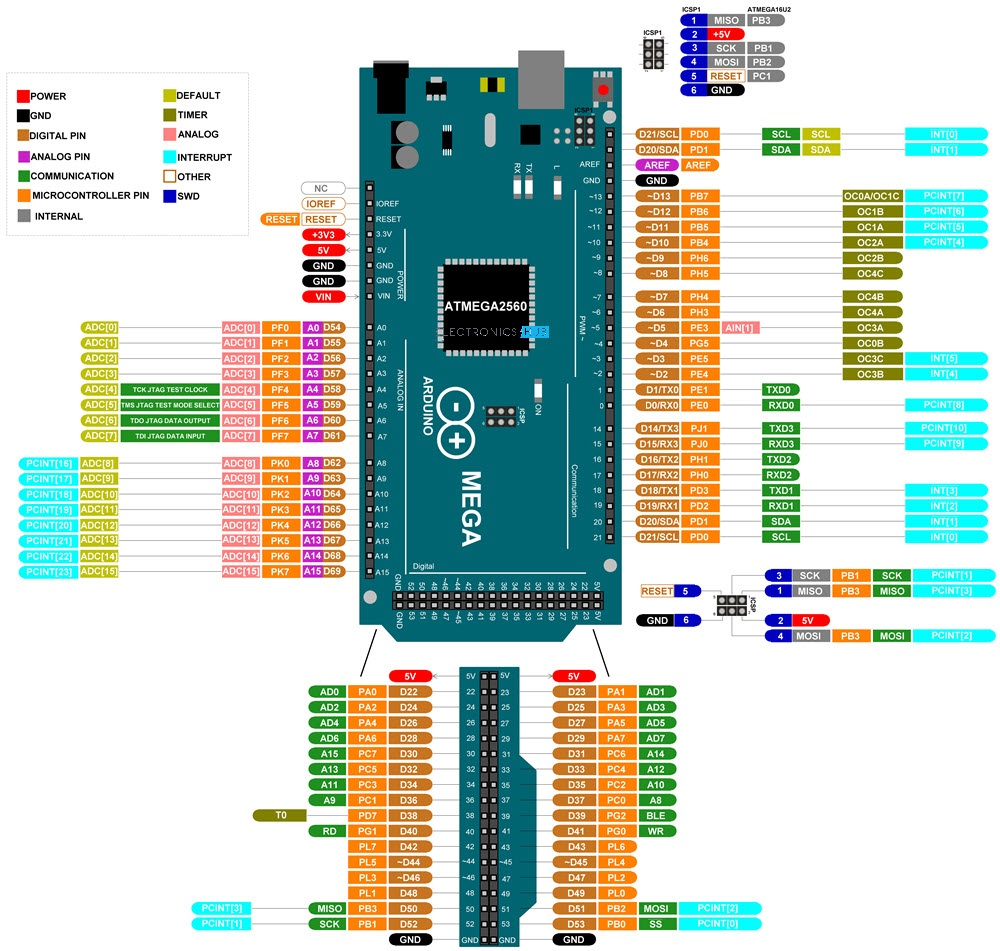
\includegraphics[height=6in]{learning_materials/Arduino-Mega-Pinout.jpg}
        \caption[Arduino Mega Pinout]{The pinout for the Arduino Mega. Retreived from \href{https://www.electronicshub.org/wp-content/uploads/2021/01/Arduino-Mega-Pinout.jpg}{Electronics Hub}}
        \labfig{arduino_mega_pinout}
    \end{figure*}

    \pagebreak % Force material past the previous section
    \subsection*{MAX7219 LED Matrix Module}
    The MAX7219 is a common cathode LED driver IC that has a four wire serial interface compatible with all microcontrollers.
    The IC is capable of driving up to 64 LEDs making it perfect for driving dot matrix displays and 7-segment displays.
    It also has a built-in BCD decoder and 64-byte static RAM which makes it very easy to display numbers, letters, or symbols on a dot matrix or 7-segment display.

    \begin{figure}[h!]
        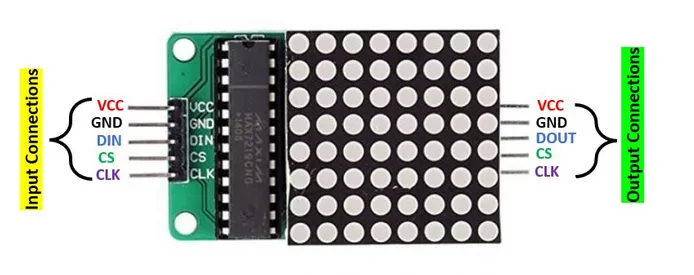
\includegraphics[]{learning_materials/MAX7219-led-matrix-pin-out.png}
        \caption[LED Matrix Pinout]{The pinout for the 8x8 LED dot matrix present in the Arduino Mega Starter Kit. 
        Retreived from \href{https://microcontrollerslab.com/wp-content/uploads/2021/09/MAX7219-led-matrix-pin-out.jpg?ezimgfmt=ng:webp/ngcb1}{Microcontrollers Lab}}
        \labfig{led_matrix_pinout}
    \end{figure}

    \marginnote{Additional information on the MAX7219 can be found here: \url{https://microcontrollerslab.com/max7219-8-digit-led-display-driver/}}

    For this particular kit, the MAX7219 drives an LED dot matrix with 8 rows and 8 columns (64 LEDs total). 
    Each LED is addressible by its particular row and column number.
    As seen in Figure \ref{fig:led_matrix_schematic}, the positive terminal of the LED "dot" is connected to a row pin, and the negative terminal of the dot is connected to a column pin.
    By setting a particular row to a positive voltage and a particular column to ground, we can turn on a dot.
    This matrix layout is a form of multiplexing and allows a microcontroller to drive 64 LEDs with only 16 pins!

    \begin{figure}[b!]
        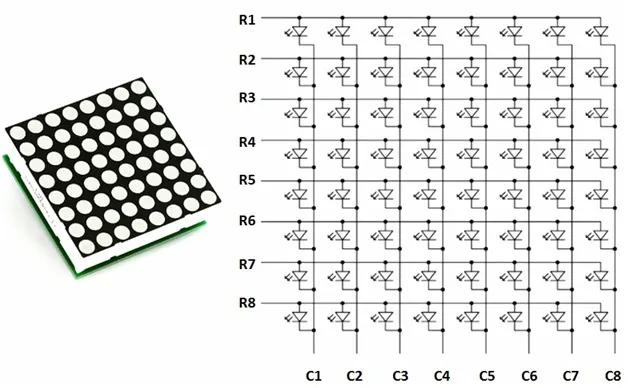
\includegraphics[height=3in]{learning_materials/led-matrix.png}
        \caption[LED Matrix Schematic]{The schematic for the 8x8 LED dot matrix present in the Arduino Mega Starter Kit. 
        Retreived from \href{https://microcontrollerslab.com/wp-content/uploads/2016/11/led-matrix.jpg?ezimgfmt=ng:webp/ngcb1}{Microcontrollers Lab}}
        \labfig{led_matrix_schematic}
    \end{figure}

    However, 16 pins is still a substantial amount for an embedded platform and computing the logic for which LEDs to turn on/off for a specific symbol wastes valuable compute cycles.
    It is much more efficient for us to use a dedicated IC like the MAX7219 to handle driving the matrix for us. 
    The IC can use its built-in serial decoder to drive all 64 LEDs from 4 pins on the microcontroller.
    It also handles all of the logic for displaying specific symbols, releiving the microcontroller from additional calculations.
    Since the MAX7219 sole purpose is to drive LED displays, it can also run much faster allowing programs to display text that smoothly scrolls across the matrix with minimal interruption.
    
    The MAX7219 serial bus also supports daisy chaining so multiple LED matrices can be connected in series to make a larger overall display.\sidenote{This does come at the cost of increasing input delay with every module. Too many modules chained together can have undesirable performance.}

    \subsection*{DS3231 Real-time Clock Module}
    The DS3231 is a sophisticated real-time clock module that maintains a high time keeping accuracy over a long period of time and a range of temperatures.
    You can communicate with the DS3231 over the I2C bus which makes it extremely simple to get up and running with most microcontrollers.
    It also has a low power draw so it can be powered by a dedicated battery to ensure that projects have an accurate time keeper for data-logging, wake up interrupts, etc.

    Once you initialize the date and time on the module, you will be able to routinely get the day, month, year, day of the week, hour, minute, and second from the IC over I2C. So long as it has power, it will provide you the time.

    \begin{marginfigure}[-2in]
        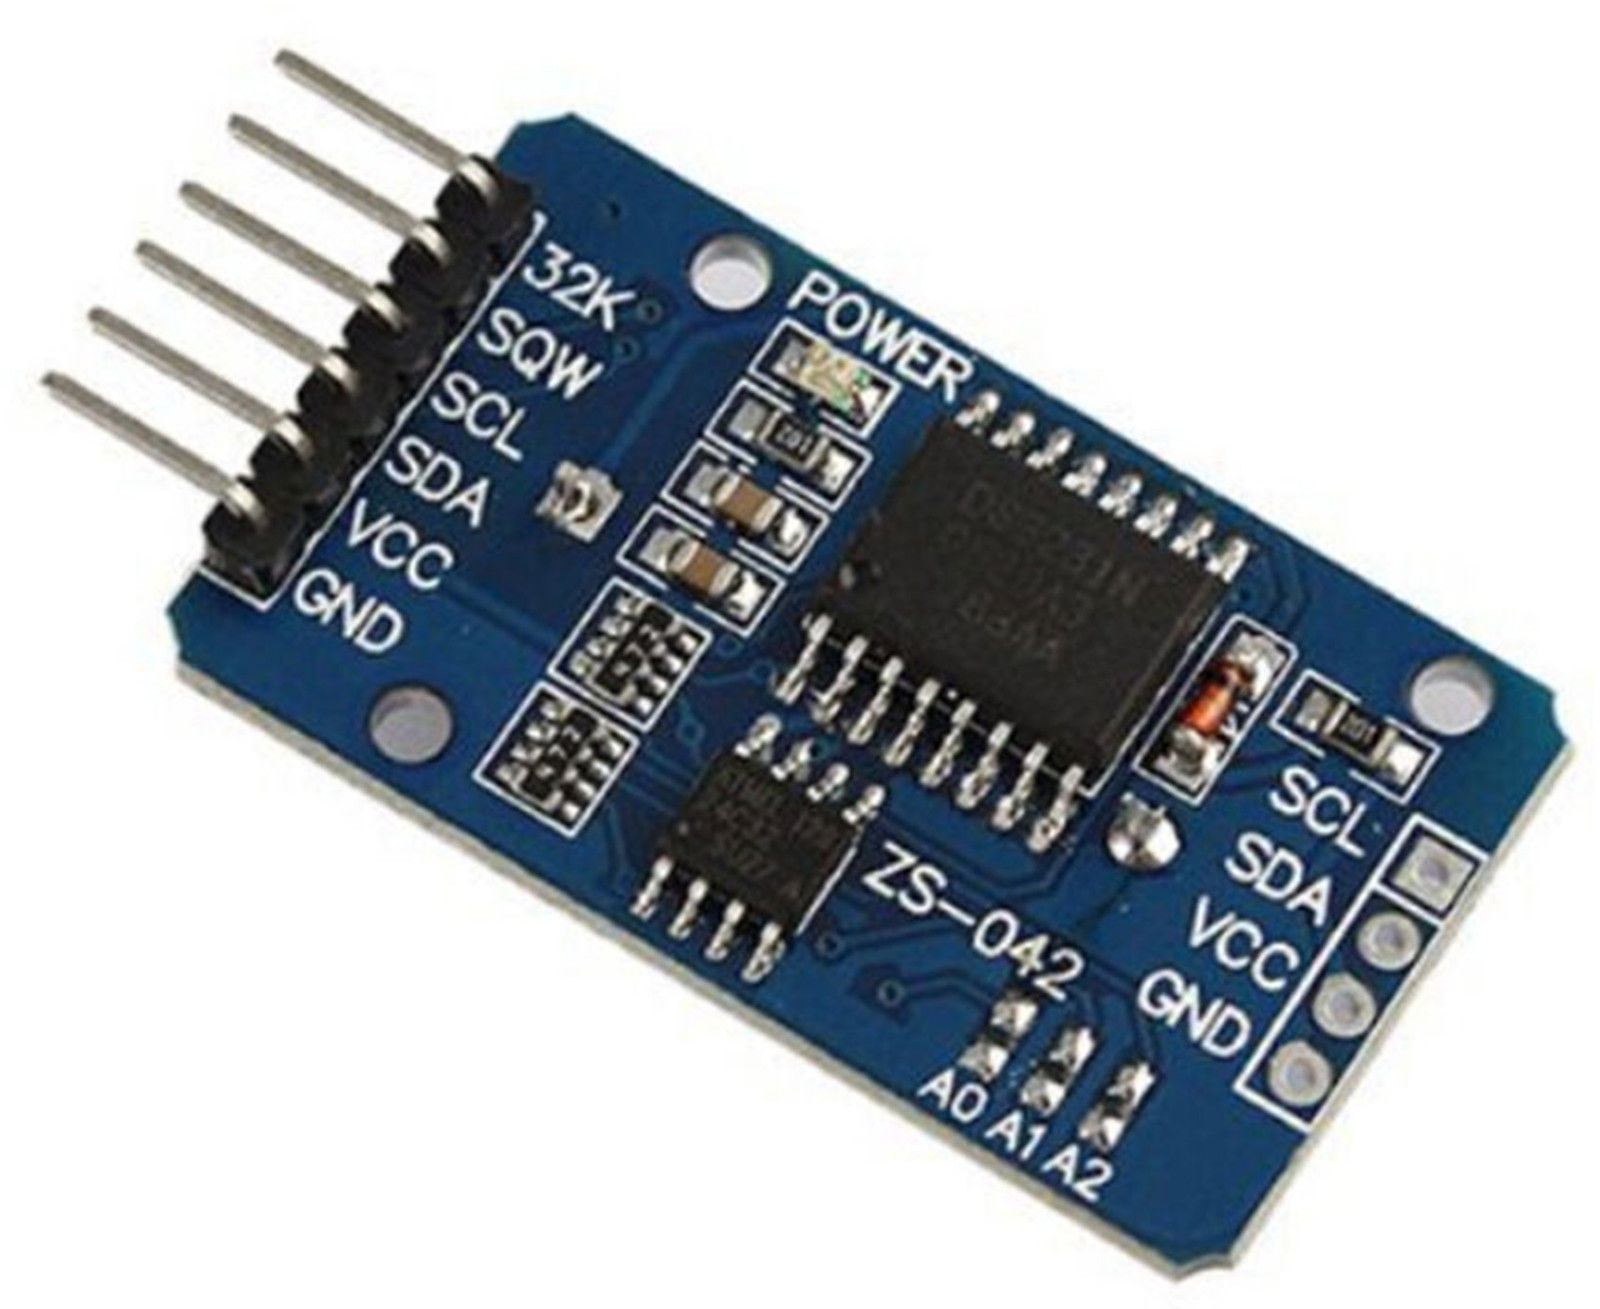
\includegraphics[]{learning_materials/ds3231-rtc.jpg}
        \caption[DS3231 RTC Module]{The DS3231 RTC module from the Arduino kit. 
        Retreived from \href{https://alltopnotch.co.uk/wp-content/uploads/imported/9/RTC-Real-Time-Clock-DS3231-I2C-AT24C32-Board-Module-Arduino-ARM-PIC-UK-Seller-361515587149-4.JPG}
        {All Top Notch}}
        \labfig{ds3231_rtc}
    \end{marginfigure}

    \subsection*{Matrix Keypad}
    The ELEGOO kit comes with a 4x4 matrix keypad with 16 individual keys.
    Much like the LED dot matrix, the keypad multiplexes the 16 buttons into four row pins, and four column pins, as shown in Figure \ref{fig:matrix_keypad}.
    In order to use the keypad, you will "scan" the matrix by connecting each column pin to an input with a pullup resistor, and each row to an output pin.
    By incrementally setting each row pin to low, and checking the input of each column pin, you can determine which button has been pressed.
    For example, if you are checking the second row of buttons by setting that pin to low and the third column pin is also low, than the button in position (2,3) (normally `6') is pressed.

    \begin{figure}[h!]
        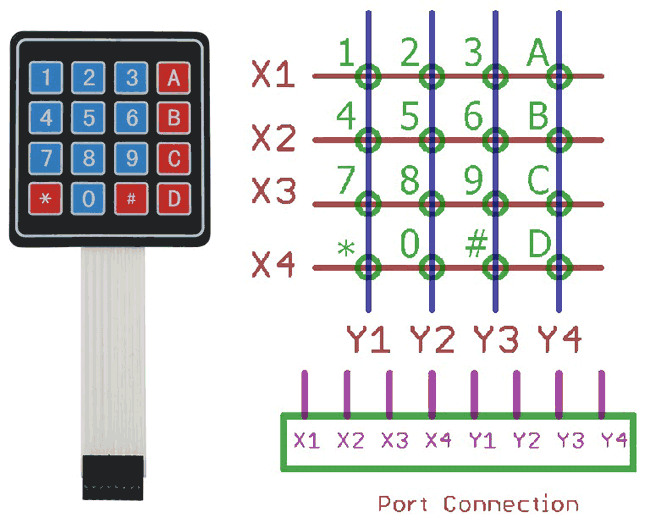
\includegraphics[height=2.5in]{learning_materials/4x4-matrix-keypad.png}
        \caption[4x4 Matrix Keypad]{The pinout and schematic for the 4x4 matrix keypad included in the Arduino starter kit. 
        Retreived from \href{https://dhaneshablogs.blogspot.com/2019/08/interfacing-4x4-matrix-keypad-with.html}
        {Dhanesha Blogs}}
        \labfig{matrix_keypad}
    \end{figure}

    \subsection*{PIR Motion Sensor}
    Passive Infrared (PIR) motion sensors detect levels of infrared radiation in their field of view.
    Inside a plastic bubble housing is a crystal that is sensative to IR radiation and is split into two halves.
    If one half of the crystal detects a different level of IR radiation than the other, the PIR driver IC will trigger a change on the interrupt line.
    This allows a microcontroller to do basic human sensing applications for monitoring foot traffic in an area, or if someone has entered/left a room.
    Additionally, the PIR sensor has some potentiometers that allow users to tweak the sensativity of the module and the time delay between triggers.

    \begin{figure}[h!]
        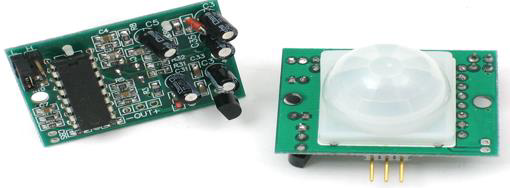
\includegraphics[height=2.5in]{learning_materials/pir_sensor.jpg}
        \caption[PIR Sensor]{The PIR sensor module included in the Arduino kit. 
        Retreived from \href{https://www.tutorialspoint.com/arduino/arduino_pir_sensor.htm}
        {Tutorials Point}}
        \labfig{matrix_keypad}
    \end{figure}

    \subsection*{IR Receiver}
    The IR receiver operates with the same physical principles as the PIR motion sensor, but has much simpler circuitry.
    Inside a small housing is a crystal that is sensitive to IR radiation.
    When the crystal is excited, it creates an electrical signal that can be read by a microcontroller on the output pin.
    All IR remotes (including the one in your Arduino kit) encode your button presses as flashes of IR light.
    When the IR receiver "sees" these flashes, it will convert them to an electrical signal with roughly the same timing as the remote output.
    This allows you to communicate with your microcontroller over light waves and signal it for different actions or functions.

    This is the same exact way older TVs and AV receivers and DVD players function. 
    Pressing a button on your remote would send an encoded signal to turn up or down the volume, change the channel, or fast forward a movie.
    Universal remotes simply were able to switch between different encoding schema for different devices.
    Can you decode the messages your TV receives?

    \begin{marginfigure}[-2.5in]
        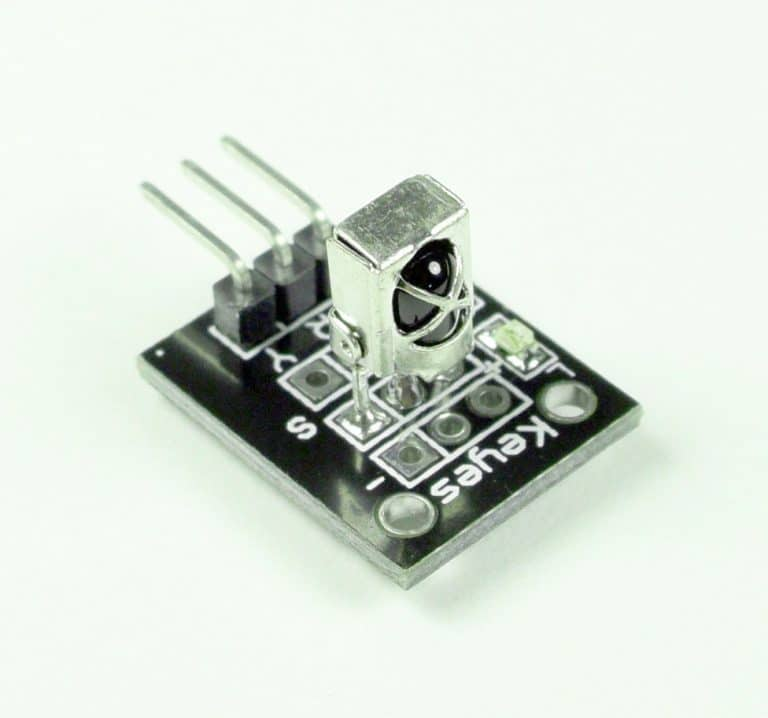
\includegraphics[]{learning_materials/ir-receiver.jpg}
        \caption[IR Receiver]{The IR receiver module included in the Arduino kit. 
        Retreived from \href{https://www.circuitbasics.com/arduino-ir-remote-receiver-tutorial/}
        {Circuit Basics}}
        \labfig{ir_receiver}
    \end{marginfigure}

    \subsection*{LCD Screen}
    \marginnote{You will become very familiar with this module in \hyperref[ch:p4_accelerometer_display]{Project 4}!}
    You kit comes with a neat module called the LCD 1602 Display.
    It can display text, images or icons in a 16-character by 2-column matrix.
    LCD stands for Liquid Crystal Display which is a technology that most screens in the world use. 
    Each character in the display is comprised of a 5x8 matrix of pixels.
    A driver IC applies an electric field to each of those specific pixels, polarizing the liquid crystal masking filter above it.
    This allows light from the backlight to be filtered through so you can see the message written on the display.
    The data used to drive the LCD is sent from the Arduino over the parallel bus which sends multiple bytes over multiple lines \textit{in parallel} to increase overall throughput.

    \begin{figure}[h!]
        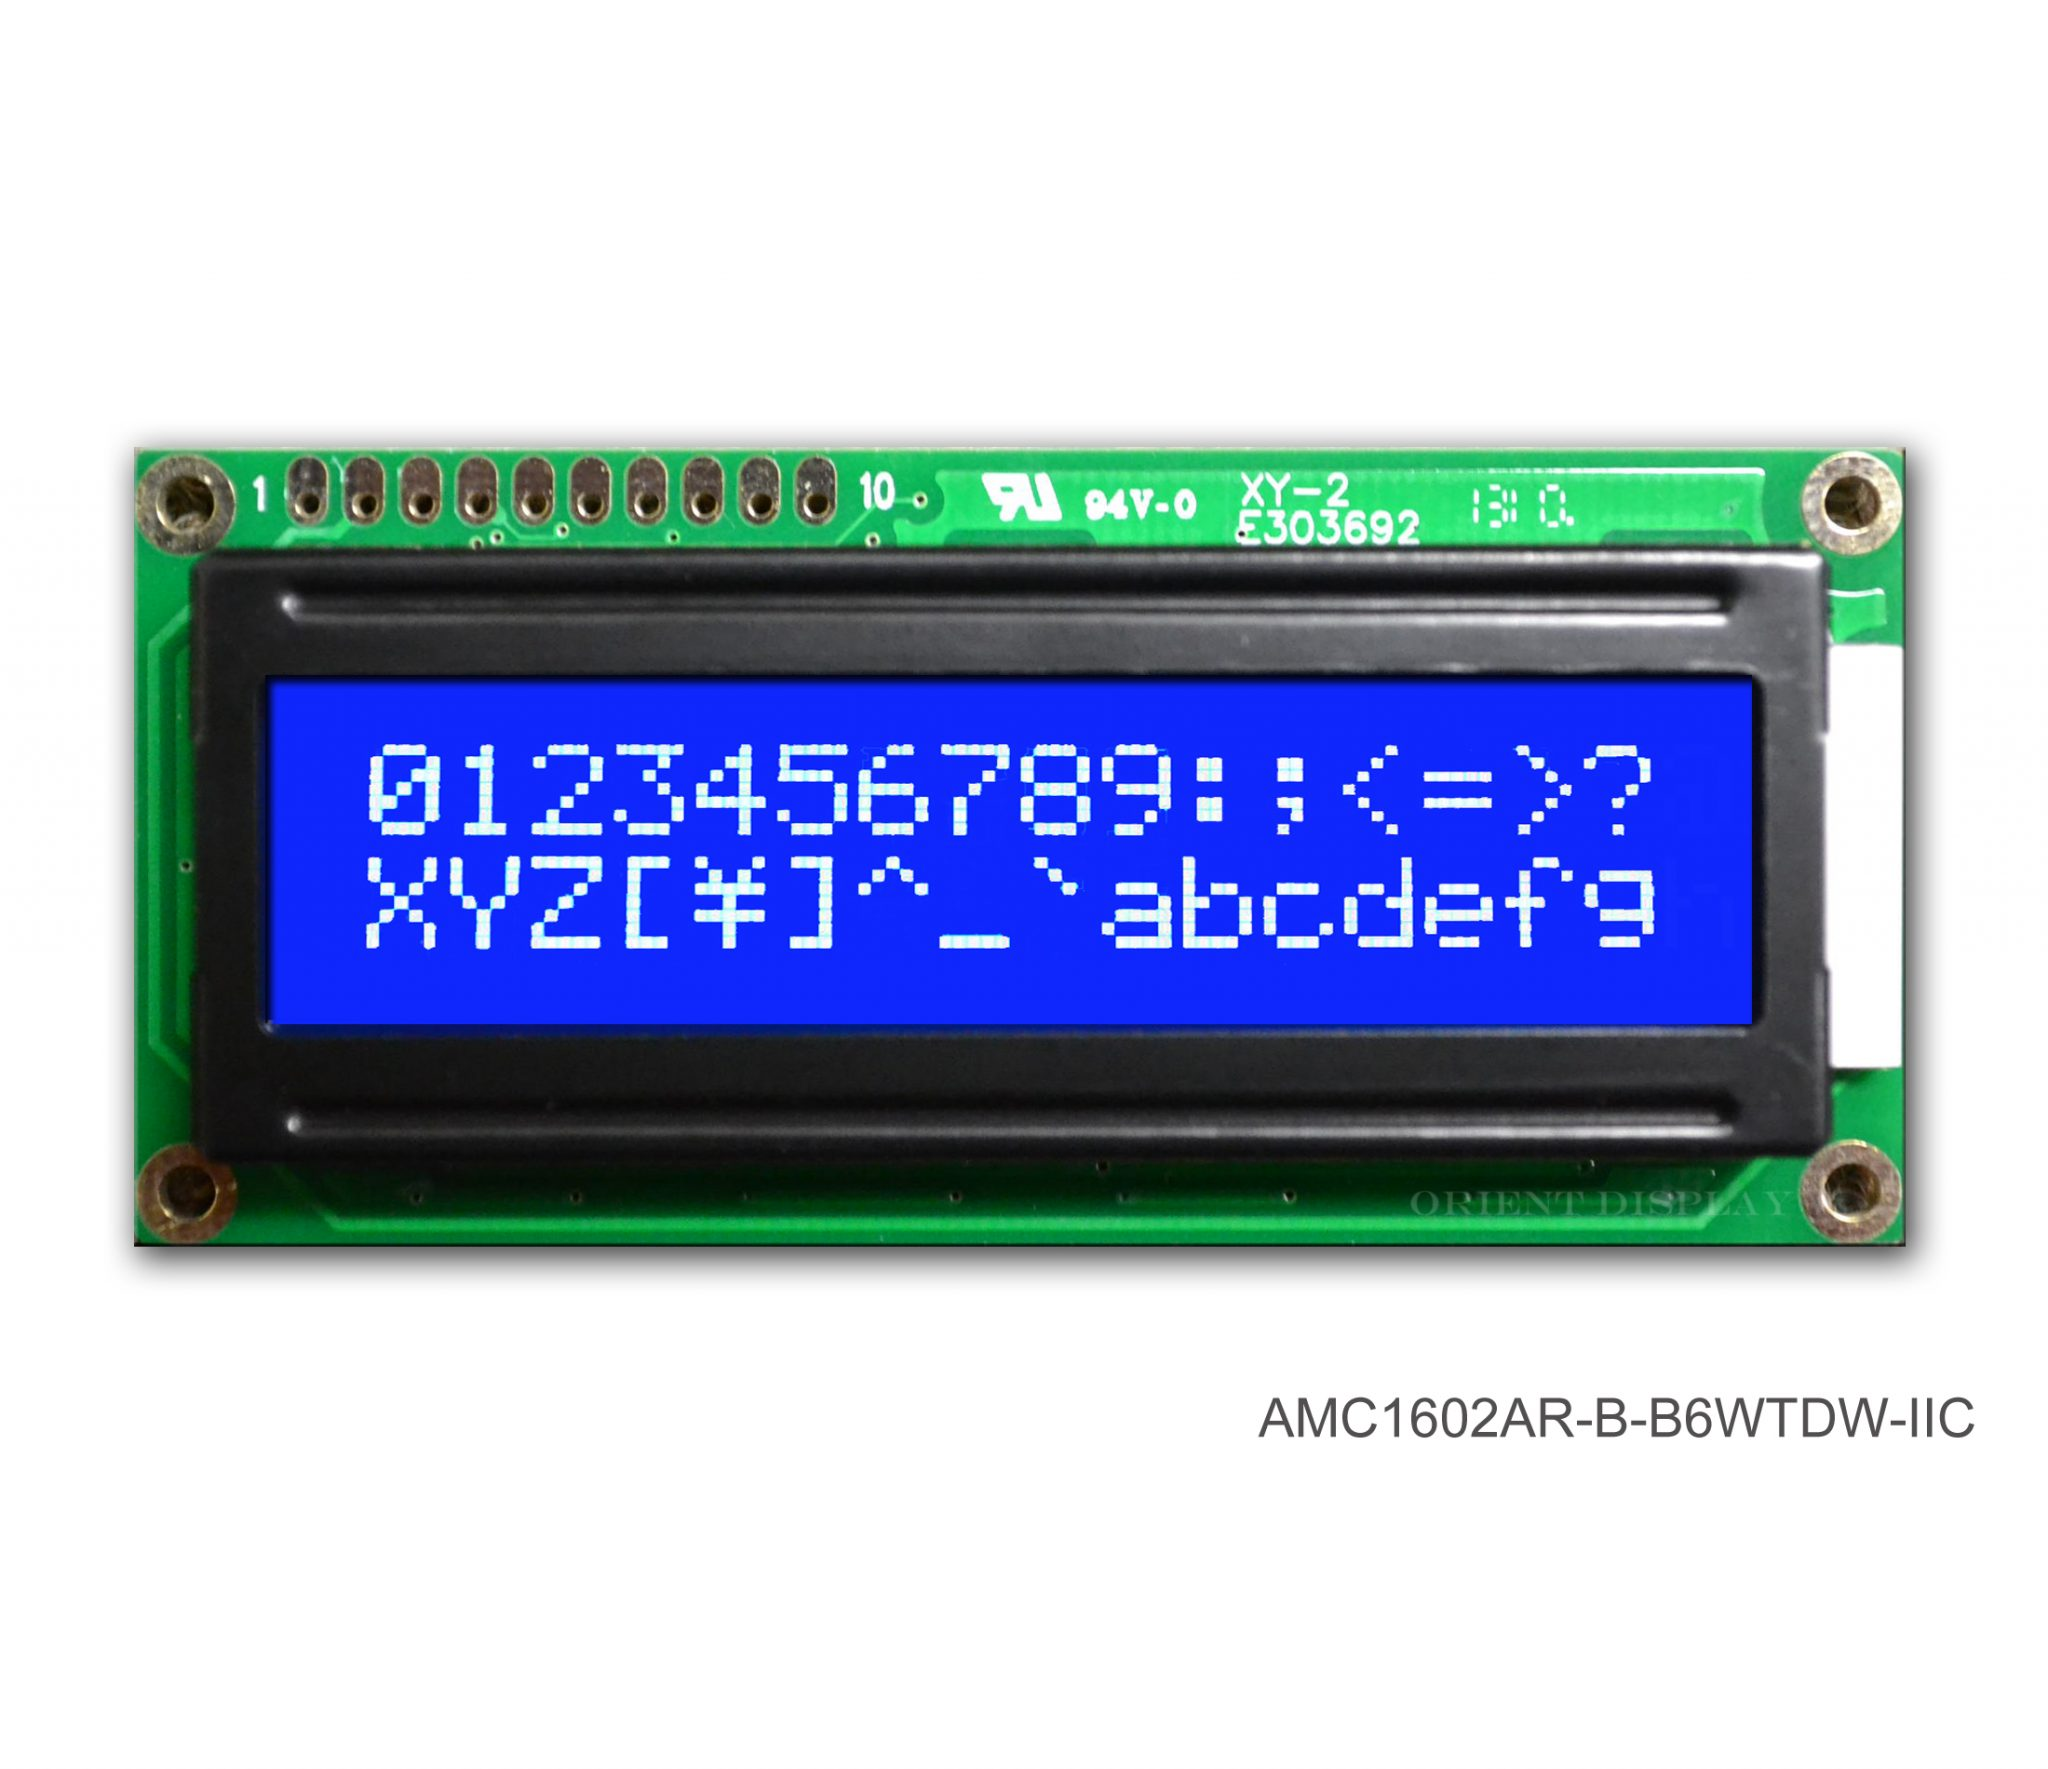
\includegraphics[height=3in]{learning_materials/lcd1602.png}
        \caption[LCD Module]{The LCD1602 module included with the Arduino kit. 
        Retreived from \href{https://www.orientdisplay.com/wp-content/uploads/2020/08/AMC1602AR-B-B6WTDW-I2C-1.jpg}
        {Orient Display}}
        \labfig{lcd_module}
    \end{figure}

    % \pagebreak % Force material past the previous section
    \subsection*{Joystick}
    The joystick is a ubiquitous human input device (HID).
    If you have every played with a game controller, you have used a joystick.
    It consists of two potentiometers: one on the x-axis and one on the y-axis, and a push button.
    These potentiometers are spring loaded to return to the center (neutral) position when no force is acting on the stick.\sidenote{You can learn more about potentiometers and joysticks in the \hl{RESISTOR SECTIONS}}
    When you push the stick forwards or backwards, the y-axis potentiometer will change the voltage on the output pin, allowing the Arduino to detect movement.
    Same goes for left and right motion on the x-axis.
    Pushing the stick in will press the built-in button, adding another input method to the Arduino.

    \begin{marginfigure}[-2in]
        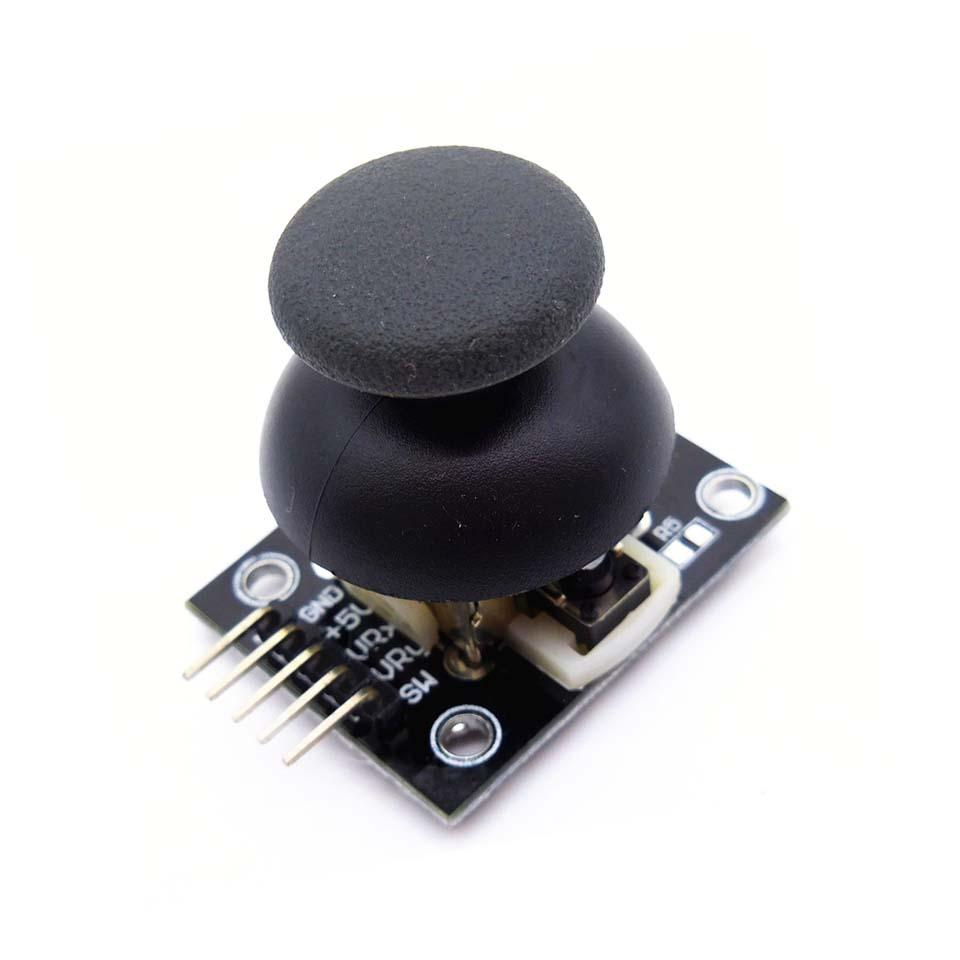
\includegraphics[]{learning_materials/joystick.png}
        \caption[Joystick]{The PS2-style dual axis joystick included with the Arduino Kit. 
        Retreived from \href{https://www.orientdisplay.com/wp-content/uploads/2020/08/AMC1602AR-B-B6WTDW-I2C-1.jpg}
        {DH Gate}}
        \labfig{lcd_module}
    \end{marginfigure}

    \subsection*{Ultrasonic Distance Sensor}
    The ultrasonic distance sensor included with your kit is a time-of-flight based tool for detecting the proximity of objects.
    Much like how a bat or dolphin uses echolocation, this sensor emits a pulse of sound for a certain duration at a certain frequency.
    The sound is emitted from the transmitter, reflects off an object, and is heard by the receiver.
    By measuring the time between the pulse being sent out and the reflected pulse being received, and knowing the speed of sound through air, we can determine the distance to an object.
    
    \begin{marginfigure}[-1.5in]
        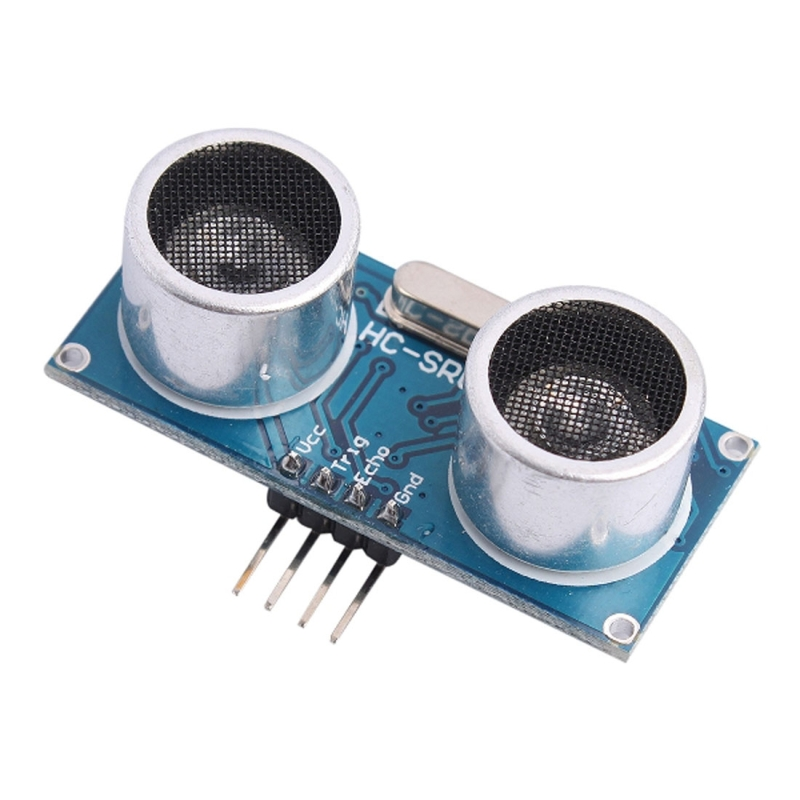
\includegraphics[]{learning_materials/ultrasonic-sensor.jpg}
        \caption[Ultrasonic Sensor]{The ultrasonic distance sensor included with the Arduino Kit. 
        Retreived from \href{https://alexnld.com/wp-content/uploads/2017/12/DIY4002_1.jpg}
        {Alexnld}}
        \labfig{ultrasonic_sensor}
    \end{marginfigure}

    \subsection*{Sound Detection Module}
    The KY-038 microphone module is a capactive microphone that is sensative to frequencies from 50-10k Hz and has an amplification circuit on-board.
    This microphone converts sound pressure waves into an electrical signal that the Arduino can read for various tasks.
    By fiddling with the sound level potentiometer on the module, a threshold sound amplitude can be controlled.
    When the microphone detects a sound above the set threshold, it will output a digital signal on an output pin.
    Additionally, there is an analog output pin which the Arduino can use to detect the amplified sound waveforms captured by the microphone.
    The pinout for this module is shown below.

    \begin{figure}[h!]
        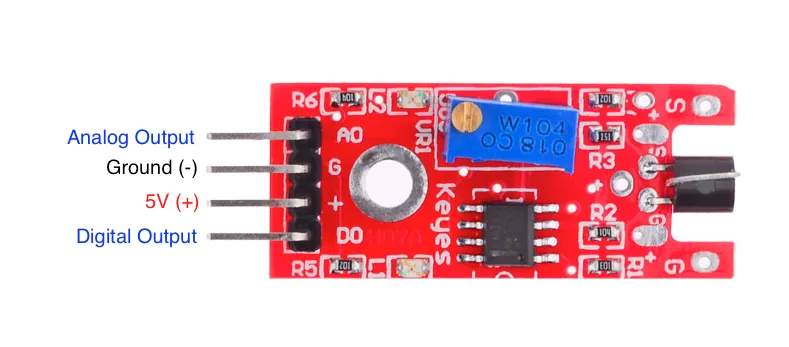
\includegraphics[height=3in]{learning_materials/sound-detection-module.png}
        \caption[Sound Detection Module]{The KY-038 sound detection module included with the Arduino Kit. 
        Retreived from \href{https://microcontrollerslab.com/ky-038-microphone-sound-sensor-module-arduino-tutorial/}
        {Micrcontrollers Lab}}
        \labfig{sound_module}
    \end{figure}

    \subsection*{ULN2003 Motor Driver Board}
    The ULN2003 stepper driver IC is a common motor driver module for stepper motors. \sidenote{You can learn more about stepper motors and how to drive them in the \hl{ACTUATORS SECTION}}
    This driver uses 4-inputs to determine what sequence to drive the stepper motor poles.
    By connecting the Arduino to these inputs and setting them high or low in a certain sequence, the ULN2003 module will "step" the motor, rotating it a precise and known amount.
    This can give you very precise control over rotational and linear motion.
    There are also a multitude of libraries available to help simplify working with this module and making precise movements.

    \begin{figure}[h!]
        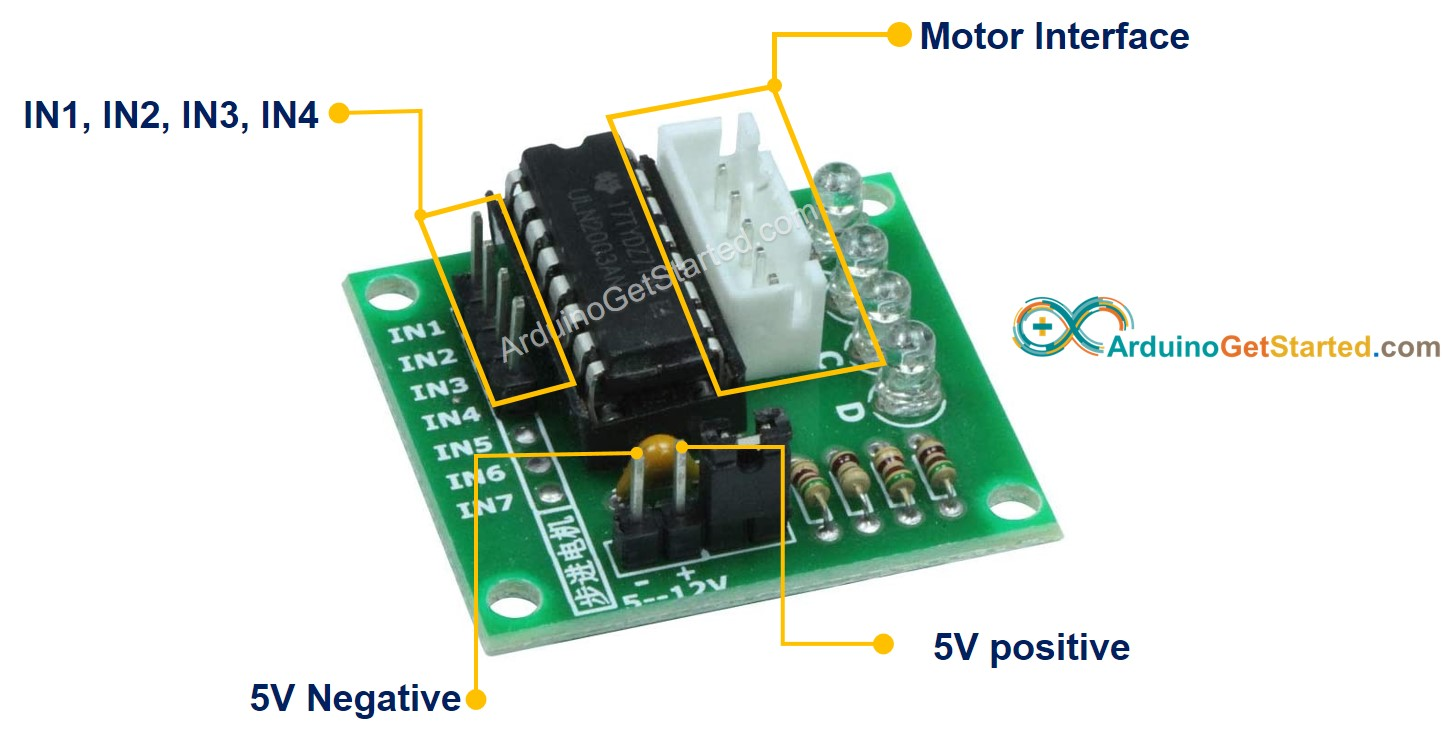
\includegraphics[height=3in]{learning_materials/uln2003-module-pinout.jpg}
        \caption[Motor Driver]{The ULN2003 motor driver board included with the Arduino Kit. 
        Retreived from \href{https://arduinogetstarted.com/images/tutorial/uln2003-module-pinout.jpg}
        {Arduino Get Started}}
        \labfig{motor_driver}
    \end{figure}

    \subsection*{DHT-11 Sensor}
    The DHT-11 sensor module features a humidity and temperature sensor combined into a signal package with a calibrated digital output.
    The temperature sensor is an Negative Temperature Coefficient (NTC)-type that reduces its resistance as temperature increases.
    The humidity sensor is a resistive-type component that changes its resistance based on the ambiant humidity.
    These sensors are connected to a small dedicated microcontroller through a amplifier network.
    The microcontroller reads in the sensor values and outputs the data over a single wire digital interface.
    Your Arduino can connect to that interface and get the ambient temperature and humidity using a multitude of libraries.
    
    \begin{figure}[h!]
        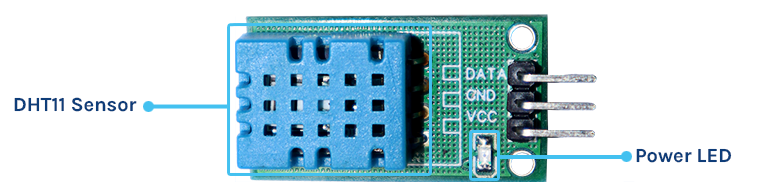
\includegraphics[height=3in]{learning_materials/DHT11-Sensor-Module-Parts.png}
        \caption[DHT-11 Sensor]{The DHT-11 temperature and humidity sensor included with the Arduino Kit. 
        Retreived from \href{https://circuitdigest.com/sites/default/files/inlineimages/u4/DHT11-Sensor-Module-Parts.png}
        {Circuit Digest}}
        \labfig{dht11_sensor}
    \end{figure}

    \subsection*{Water Level Sensor}
    The water level sensor has a series of ten traces exposed on its PCB; five are power traces, five are sense traces.
    These traces are interlaced such that they are not connected until they are submerged in water and bridged together.
    As the water level increases, more sense traces are connected to more power traces and thus, the overall resistance of the circuit is decreased.
    This resistance is inversely proportional to the water level (i.e. as the water level increases, the resistance wll decrease).
    By measuring the voltage across the sensing pin and ground, we can correlate the water level to the voltage reading, much like we would with a potentiometer.
    One caveat though is that constantly powering the sensor while it is submerged will dramatically increase the galvonic corrosion and reduce the sensor's lifespan.
    Therefore the positive voltage pin should only be driven high when a reading is actively being taken.

    \begin{figure}[h!]
        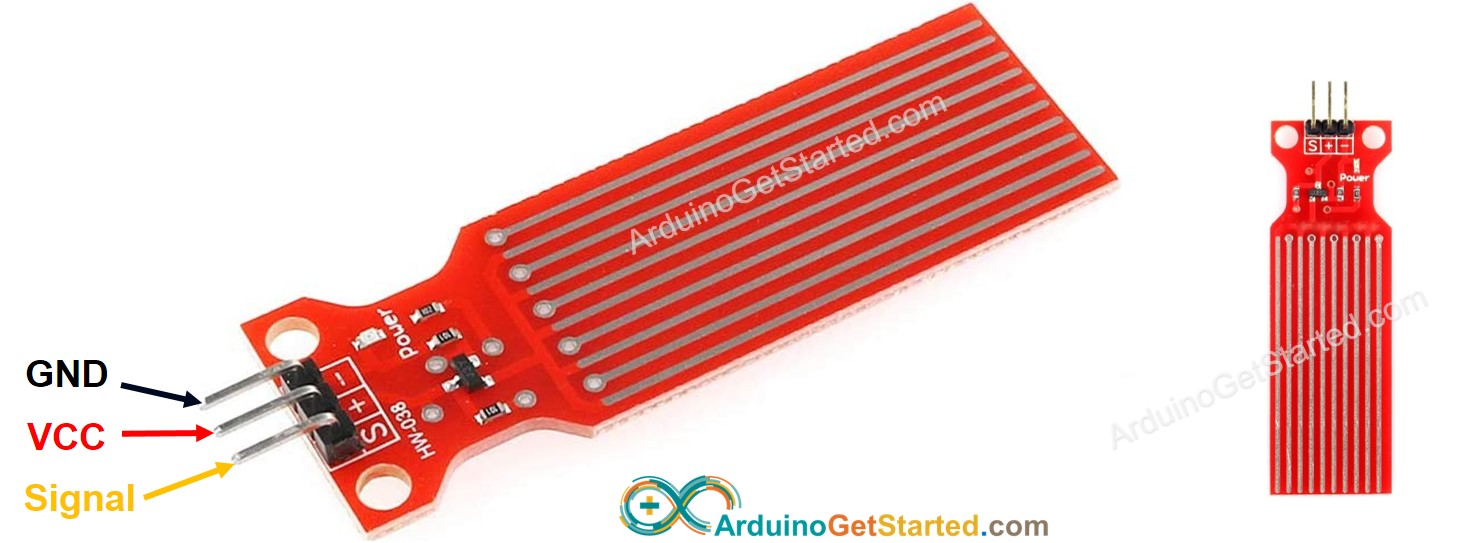
\includegraphics[height=3in]{learning_materials/water-sensor-pinout.jpg}
        \caption[Water Level Sensor]{The water level sensor included with the Arduino Kit. 
        Retreived from \href{https://arduinogetstarted.com/images/tutorial/water-sensor-pinout.jpg}
        {Arduino Getting Started}}
        \labfig{dht11_sensor}
    \end{figure}

    \subsection*{4-Digit 7-Segment Display}
    \marginnote{You will become very familiar with this module in \hyperref[ch:p3_7seg_counter]{Project 3}!}
    The 4-digit 7-segment display is a series of 7-segment displays connected together in parallel with a common cathode.
    Much like the keypad and LED dot matricies, this module can display different numbers and values based off which lines are turned on or off.
    There are four "digit" lines that are connected to the annode of their respective digit.
    Driving these lines high, while pulling one of the display LEDs low will cause that LED to illuminate.
    For example, to display a "0" in the first digit, you would drive the first digit pin high, and pull the LEDs pins A-F low, illuminating a "0".

    On the Arduino, it can be inconvient to connect so many data lines, so often, a shift register like the 74HC595 is used to drive the display LEDs, while the Arduino controls which digits are activated.

    \begin{figure}[h!]
        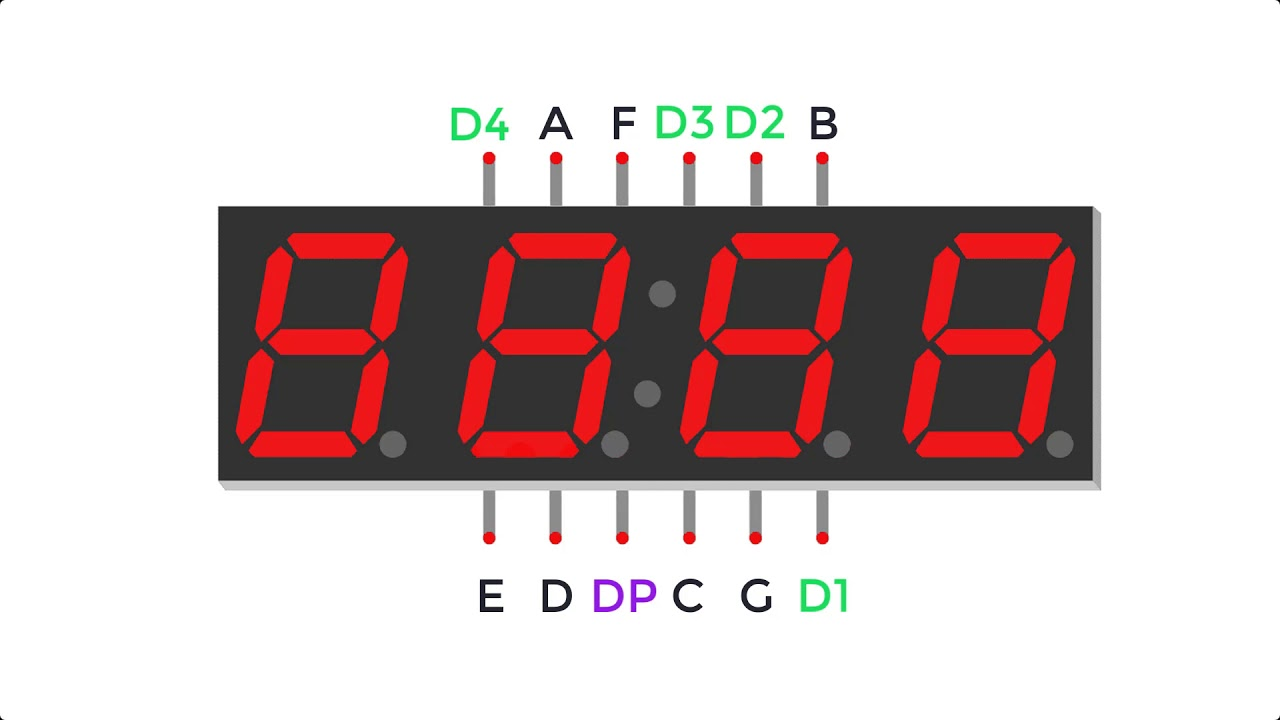
\includegraphics[height=3in]{learning_materials/4-digit-7-segment-display.png}
        \caption[4-Digit 7-Segment]{The 4-digit 7-segment display included with the Arduino Kit with pinout. 
        Retreived from \href{https://i.ytimg.com/vi/fYAlE1u5rno/maxresdefault.jpg}
        {Make Crate}}
        \labfig{4digit_7seg}
    \end{figure}

    \begin{figure*}[b]
        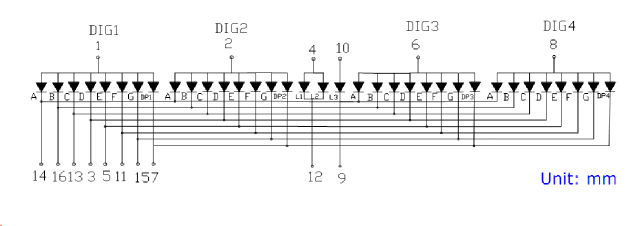
\includegraphics[height=3in]{learning_materials/arduino-4-digit-7-segment-insides.png}
        \caption[4-Digit 7-Segment Schematic]{The inside schematic of the 4-digit 7-segment display. 
        Retreived from \href{https://lh6.googleusercontent.com/-UVNbhMgaoc4/Thh-bH7d5zI/AAAAAAAAAEQ/FphoqjmYsVg/s800/arduino-4-digit-7-segment-insides.png}
        {All About EE}}
        \labfig{4digit_7seg_sch}
    \end{figure*}

% ===========================================
% Digital Logic
% Written by: Braidan Duffy
%
% Date: 07/06/2022
% Last Revision: 07/25/2022
% ============================================

\setchapterstyle{kao}
\chapter{Digital Electronics}
\setchapterpreamble[u]{\margintoc}
\labch{digital_electronics}

Computers have existed in some fashion or another for millennia.
The ancient antikythera mechanism was a hand-powered computer that predicted the position of astronomical bodies throughout the year.
Mathematicians in the 18th and 19th centuries used complicated machines and mechanisms to run calculus and trigonometric calculations at speeds way faster than possible by humans by hand.
Then, in the mid-1940's nations used analog computers to compute the trajectories of ballistic projectiles and free falling bombs.
Today, analog computers are still used in niche applications, but since the transistor revolution of the 1960's and 1970's, almost every computer in the world has transitioned to digital logic.

\section[Introduction to Binary]{Introduction to Binary}
Digital logic is electrically simple to implement: either current flows (a logical '1') or it does not (a logical '0').
Even better, the circuit required to calculate digital logic can be generalized or reconfigured, depending on the architecture used.
This makes digital logic a far more versatile tool compared to analog computers which can only be made for specific applications.

The fundamentals of computing are above the scope of these notes, but it is still important for engineers to understand the basic logic behind digital computations and know about the 1's and 0's that dictate our modern lifestyles

\paragraph*{What is Binary?} Binary is the representation of the state of an object.
As the latin prefix implies, there are two states represented by binary: on (logical '1') or off (logical '0').
A lightbulb is a good example of a binary object - it is either on, lighting up a room, or off, leaving the room in darkness.

Binary is fundamentally a numbering system, much like the arabic numerals we use in our day-to-day lives.
Arabic numerals are in Base10, meaning we comprehend counting in multiples of 10 using the digits 0-9. For example:
\begin{align*}
    20     &= 10*2 \\
    450    &= 4*10*10 + 5*10 \\
    245683 &= 2*10^5 + 4*10^4 + 5*10^3 + 6*10^2 + 8*10^1 + 3*10^0
\end{align*}

Binary is counted in Base2, meaning everything is counted in multiples of 2 using the digits 0 and 1. Using the same example as before:
\begin{align*}
    20     &= 2^4 + 2^2 \\
    450    &= 2^8 + 2^7 + 2^6 + 0^5 + 0^4 + 0^3 + 0^2 + 2^1 + 0^0 \\
    245683 &= 2^{17} + 2^{16} + 2^{15} + 2^{13} + 2^{12} + 2^{11} + 2^{10} + 2^9 + 2^8 + 2^7 + 2^5 + 2^4 + 2^1 + 2^0
\end{align*}
        
While this is inefficient for a human to understand its meaning, a computer can quickly transform this on/off pattern of electrons into numbers for calculations.

Binary numbers are broken down into three groupings: bits (one number), nibbles (four bits), and bytes (two nibbles or eight bits). 
The groupings are extremely important as the order and number of the bits in a binary representation dictate the number or logical input used in the calculation.
Each bit is indexed starting from 0, as shown in \hl{FIGURE} and goes from the Least Significant Bit (LSB) at index 0, to the Most Significant Bit (MSB) at the furthest index. 
\sidenote{These indecies get their names because of how they affect the binary number when changed. 
The LSB only changes the numerical value by 1.
The MSB, on the other hand, can change the value by upto an infinite value, depending on how many bits are present in the binary number}

\begin{figure*}
    \labfig{byte_breakdown}
    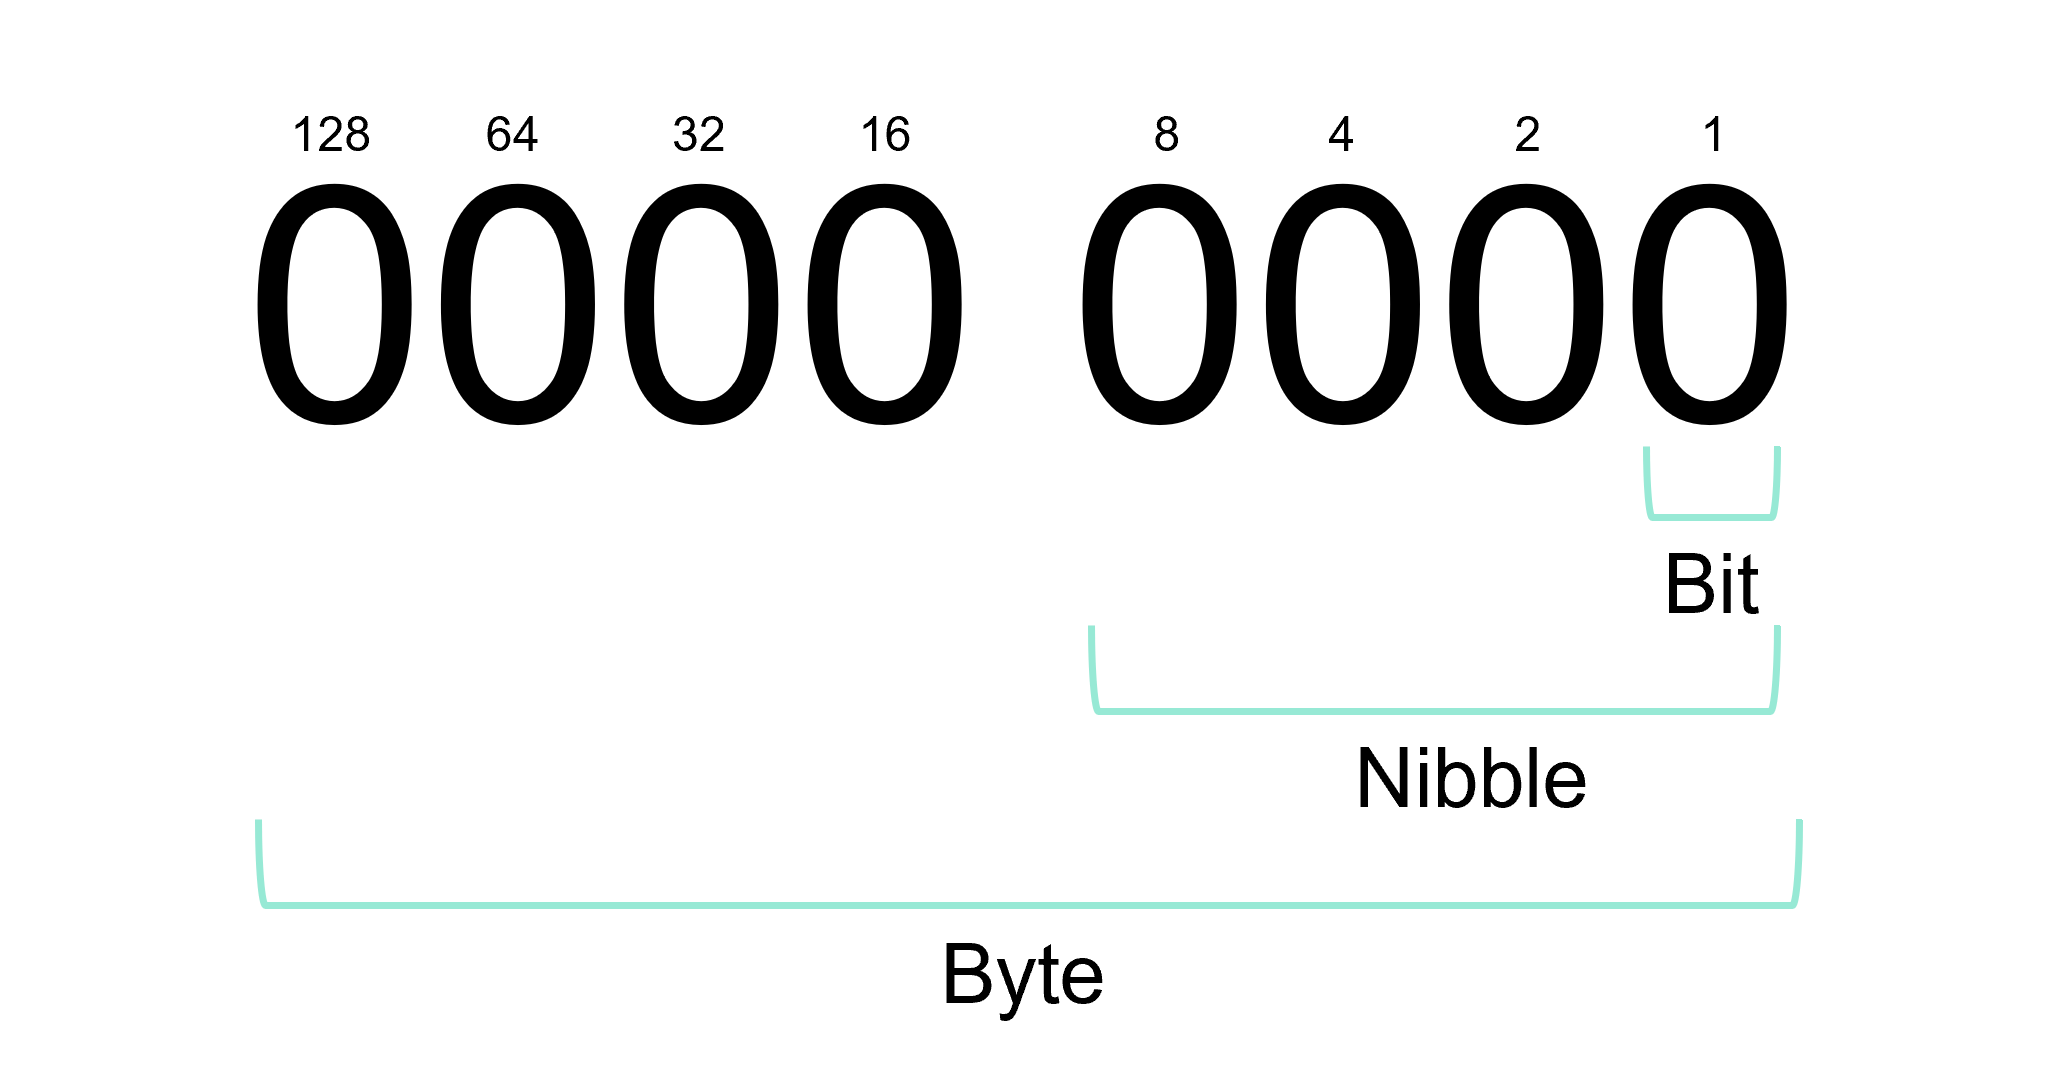
\includegraphics[height=2.5in]{digital_logic/bit-breakdown.png}
    \caption[Byte Breakdown]{Breakdown of a byte from the largest unit, to the smallest, with indexing.}
\end{figure*}

% \pagelayout{wide} % Remove margins

\begin{example}
    Let's take a look at a practical demonstration of binary using your Arduino kit.
    You will need:
    \begin{itemize}
        \item 1 x Red LED
        \item 1 x button
        \item 1 x 220 $\Omega$ resistor
        \item 2 x Male-to-Male jumper wires
    \end{itemize}

    Wire these components to a breadboard like so:
    % \begin{figure}
        
    % \end{figure}

    The dfault state for this system should be active high, meaning the LED will be off when the button is not pressed - a logical 0.
    When you press the button, you push the system to the high state and turn on the LED - a logical 1!
\end{example}

% \pagelayout{margin} % Restore margins

    \subsection{Binary Arithmetic}
    Much like our beloved arabic numerals, binary numbers can be added, subtracted, multiplied, and divided.

    \paragraph*{Addition} Adding binary numbers is straight-forward.
    Simply stack the numbers you wish to add on top of each other, ensuring the indices align.
    Note, binary addition is commutative, meaning the number order does not matter, so long as the indices are aligned.
    Then, for each index, add the numbers together.
    If the result is greater than 1, then set the result of the index addition to 0 and carry a '1' over to the next index.
    Repeat until you have calculated the last index!

    \begin{example}[Adding binary numbers]
        Let's add $7_{10}$ ($0111_2$) and $11_{10}$ ($1011_2$):
        \begin{center}
            \begin{tabular}{ccccc}
                $^1$  & $0^1$ & $1^1$ & $1^1$ & $1$ \\
                +     & 1     & 0     & 1     & 1 \\
                \hline
                1     & 0     & 0     & 1     & 0 \\
            \end{tabular}
        \end{center}
    \end{example}

    \paragraph*{Subtraction} Subtracting binary numbers is simply the same algorithm for Base10 numbers.
    Starting at the LSB, subtract the two numbers index-by-index.
    If a case arises, when the subtrahend \sidenote{bottom number} has a larger number than the same index in the minuend \sidenote{top number}, borrow a '1' from the next index.
    If you are are unable to borrow a '1', grab one from the next index until you can get a '1' to bring back.
    When you bring a '1' back, then perform the subtraction.
    Repeat this process until you have calculated the last index.
    
    \begin{example}[Subtracting binary numbers]
        Let's subtract $24_{10}$ ($11000_2$) and $7_{10}$ ($111_2$):
        \begin{center}
            \begin{tabular}{cccccc}
                  & 1 & $1^0$ & ${0^{10}}^1$ & ${0^{10}}^1$ & ${0^{10}}^1$  \\
                - & 0 & 0     & 1            & 1            & 1             \\
                \hline
                  & 1 & 0     & 0            & 0            & 1             \\
            \end{tabular}
        \end{center}
    \end{example}

    \begin{kaobox}[frametitle=Aside: 2's Complement Method]
        The above method is easy for humans to understand, but computationally expensive. 
        For operations that require borrowing, many repetitive borrow operations are performed, wasting CPU cycles.
        Instead, computers use a complement method to simplify the subtraction operation and increase performance.

        Here, we are going to perform the same calculation as before. Begin by aligning the two numbers as previously, "padding" \sidenote{adding leading zeroes, as necessary} both numbers so they are the same length.
        
        \begin{center}
            \begin{tabular}{cccccc}
                  & 1 & 1 & 0 & 0 & 0 \\
                - & 0 & 0 & 1 & 1 & 1 \\
                \hline
            \end{tabular}
        \end{center}

        Then, switch all of the bits in the subtrahend. In this case, 00111 becomes 11000. \sidenote{What is occuring here is known as the 1's complement as we are subtracting '1' from each bit in the number. This only works in binary}
        Then, we are going to add 1 to the switched term:
        \begin{equation*}
            11000 + 1 = 11001
        \end{equation*}
        We are then going to change the math problem from subtraction to addition and add the original minuend and the new, switched subtrahend.

        \begin{center}
            \begin{tabular}{cccccc}
                  & 1 & 1 & 0 & 0 & 0 \\
                + & 1 & 1 & 0 & 0 & 1 \\
                \hline
                \cancel{1} & 1 & 0 & 0 & 0 & 1 \\
            \end{tabular}
        \end{center}

        To finish the algorithm, remove the MSB from the resultant. 
        You can compare this number to the previous calculation and notice that the final result is the same, depite the radically different method.
        Even though the complement method is unintuitive for humans to understand, it is vastly superior for a computer to execute as the number of required operations is dramatically smaller than the original method, even with larger values.
    \end{kaobox}

    \paragraph*{Multiplication} Binary multiplication occurs in the same order as decimal long multiplication.
    It is a commutative process, like addition, but in order to reduce the number of steps required, it is recommended that the number with the least amount of bits is the multiplicand \sidenote{bottom number} and the other factor is the multiplier \sidenote{top number}.
    For the operation, you will multiply the multiplier by each bit of the multiplicand to calculate an intermediate value.
    With every new index of the multiplicand, shift the resulting product over one bit until you have calculated the intermediate product for the last index of the multiplicand.
    Simply add all the intermediate products together to calculate the final result.

    \begin{example}[Multiplying binary numbers]
        Let's multiply $14_{10}$ ($1110_2$) and $3_{10}$ ($0011_2$):
        \begin{center}
            \begin{tabular}{cccccccc}
                  &   &   & 1 & 1 & 1 & 0 \\
                  &   & * & 0 & 0 & 1 & 1 \\
                \hline
                  &   &   & 1 & 1 & 1 & 0 \\
                  &   & 1 & 1 & 1 & 0 &   \\
                  & 0 & 0 & 0 & 0 &   &   \\
                0 & 0 & 0 & 0 &   &   &   \\
                \hline
                0 & 1 & 0 & 1 & 0 & 1 & 0 \\  
            \end{tabular}
        \end{center}
        This leaves us with the answer to the life, the universe, and everything: $0101010_2$ ($42_{10}$).
    \end{example}

    \paragraph*{Division} Binary division works exactly like decimal long division.
    You start with a dividend within the division operator and a divisor operating on it.
    Compare the divisor to the first digit of the dividend; if the divisor is larger, than a '0' is placed above the first index of the dividend, if it is smaller, than a one goes there.
    If the latter case occurs, subtract the section of the dividend from the dividend and continue the dividing operation with this new value.

    \begin{example}[Dividing binary numbers]
        Let's divide $69_{10}$ ($0100 0101_2$) by $3_{10}$ ($0011_2$):
        \[
        \begin{array}{ rr@{} >{\color{red}}c@{}*{6}{c@{\mkern2mu}} }
            & 00010111 & & & &  &  \\ \cmidrule[0.6pt](l{-0.385em}){2-8}\\[-16.9pt]
            0011\;\rlap{\Large)} & 01000101 & & & & & &  \\
            & -11~~~~~~~~~ & & & & & &  \\ 
            \cmidrule(l{1ex}){2-4}
            & 101~~~~~\\
            & -11~~~~~\\ 
            \cmidrule(l{1ex}){2-4}
            & 0100~~~ \\
            & -11~~~ \\
            \cmidrule(l{1ex}){2-4}
            & 11 \\
            & -11 \\
            \cmidrule(l{1ex}){2-4}
            & 0
        \end{array}
        \]
        This is the exact same operation performed in Base10 long division, just everything is in Base2. As you can see, the division leaves us with the correct answer of $10111_2$ ($23_{10}$).
    \end{example}

\section[Logic Gates]{Introduction to Logic Gates}
Logic gates are the building blocks of digital circuits.
An arrangement of gates grants you a specific output for corresponding sets of inputs.
This allows you to "construct" logical equations with visual representations or even physical devices.

    \subsection{Truth Tables}
    It is sometimes inefficient to display a logic flow with a diagram of gates and wires, as shown in \hl{FIGURE}. \todo{Create a figure a bunch of logic gates wired together}.
    So, these flows can be summarized by a truth table as show in in \hl{TABLE}.
    This shows the input parameters and the corresponding outputs.
    These tables can also be helpful in designing the logic diagram when given a problem.

    To setup this table, dedicate a column to each input into your system and have a column for the outputs.
    The LSB will be the column before the output column and the columns will increase in significance to the left.
    Then, for every row in the input columns, start at 0 and alternate between 0 and 1 at a specific interval.
    This interval is dictated by the index (column) of the input bit.
    The LSB will switch every row (0,1,0,1, etc.), the next bit will switch every other row (0,0,1,1, etc.), the next bit will alternate every 4 rows (0,0,0,0,1,1,1,1, etc.), and so on and so forth.
    Then, in your output column, place a 1 where you want the gates to output a logical 1 given a set of inputs.

    For example, lets design an alarm system for a fire place.
    This specific system has four alarms of various types that output a logical 1 when they detect excessive smoke from the fireplace.
    However, these sensors are known to be a little too sensitive and give false positives.
    To prevent the fire department from unnecessarily coming to the rescue, we will not sound the general alarm until two or more sensors detect excessive smoke.
    Therefore, we will construct a truth table like so:

    \begin{table}
        \labtab{truth_table_ex}
        \begin{tabular}[]{c c c c | c}
            \toprule
            Sensor 4 & Sensor 3 & Sensor 2 & Sensor 1 & Output  \\
            \midrule
                0    &    0     &    0     &    0     &    0    \\
                0    &    0     &    0     &    1     &    0    \\
                0    &    0     &    1     &    0     &    0    \\
                0    &    0     &    1     &    1     &    1    \\
                0    &    1     &    0     &    0     &    0    \\
                0    &    1     &    0     &    1     &    1    \\
                0    &    1     &    1     &    0     &    1    \\
                0    &    1     &    1     &    1     &    1    \\
                1    &    0     &    0     &    0     &    0    \\
                1    &    0     &    0     &    1     &    1    \\
                1    &    0     &    1     &    0     &    1    \\
                1    &    0     &    1     &    1     &    1    \\
                1    &    1     &    0     &    0     &    1    \\
                1    &    1     &    0     &    1     &    1    \\
                1    &    1     &    1     &    0     &    1    \\
                1    &    1     &    1     &    1     &    1    \\
            \bottomrule
        \end{tabular}
    \end{table}

    As you can see in Table \ref{tab:truth_table_ex}, for every row where two or more sensors are sending an alarm signal, the output (general alarm) is sending out a signal as well.

    \subsection{Basic Logical Operators}
    In logic, we can write a flow like an equation with a series of operators and notations that determine what outputs will result from given inputs.
    The basic operators are \textbf{AND}, \textbf{OR}, and \textbf{NOT}.
    
    \paragraph*{AND} is a basic logical operation.
    If the input 1 \textit{and} input 2 are both true (logical '1'), then the output is also true.
    Otherwise, the output is false.
    This can be represented by the equation below where $A$ is input 1 and $B$ is input 2.

    \begin{equation*}
        A \cdot B
    \end{equation*}

    And the truth table:
    \begin{table}[h!]
        \labtab{and_truth_table}
        \begin{tabular}{c c | c}
            \toprule
            $A$ & $B$ & $A \cdot B$  \\
            \midrule
             0  &  0  &    0    \\
             0  &  1  &    0    \\
             1  &  0  &    0    \\
             1  &  1  &    1    \\
            \bottomrule
        \end{tabular}
    \end{table}

    Graphically, AND gates are represented by symbols like Figure \ref{fig:and_gate}.
    Wires protrude from the three pins on the gate and "carry" information to and from other gates on the same diagram.
    \begin{figure}[h!]
        \labfig{and_gate}
        
\includegraphics[height=1in]{digital_logic/AND_gate.png}
        \caption[AND Gate]{Visual representation of the AND logical operation with two inputs and one output.}
    \end{figure}

    \paragraph*{OR} is another basic logical operation.
    It is the inverse of the AND operation as the logical output will be true when any input is true i.e. input 1 \textit{or} input 2 is true.
    It can be represented by the expression:
    \begin{equation*}
        A + B
    \end{equation*}

    With the truth table:
    \begin{table}[h!]
        \labtab{or_truth_table}
        \begin{tabular}{c c | c}
            \toprule
            $A$ & $B$ & $A+B$  \\
            \midrule
             0  &  0  &   0    \\
             0  &  1  &   1    \\
             1  &  0  &   1    \\
             1  &  1  &   1    \\
            \bottomrule
        \end{tabular}
    \end{table}

    And the visual symbol:
    \begin{figure}[h!]
        \labfig{or_gate}
        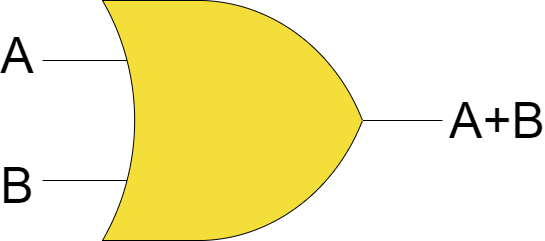
\includegraphics[height=1in]{digital_logic/OR_gate.png}
        \caption[OR Gate]{Visual representation of the OR logical operation with two inputs and one output.}
    \end{figure}

    \paragraph*{NOT} is the simplest logical operation of all.
    Simply, whatever input is passed into the NOT gate, the output will be the opposite.
    For example, a logical true input will result in a logical false output, and vice versa.
    This can be represented by the truth table:
    \marginnote{The NOT operation can be represented by either $\bar{A}$ or $!A$ where $!$ is called the "bang" operator.
    The latter operator is widely used within computer programming for the NOT operation, whereas $\bar{A}$ is more used in mathematical and handwritten expressions.}
    
    \begin{table}[h!]
        \labtab{not_truth_table}
        \begin{tabular}{c | c}
            \toprule
            $A$ & $\bar{A}$  \\
            \midrule
             0  &    1    \\
             1  &    0    \\
            \bottomrule
        \end{tabular}
    \end{table}

    And the visual symbol:
    \begin{figure}[h!]
        \labfig{not_gate}
        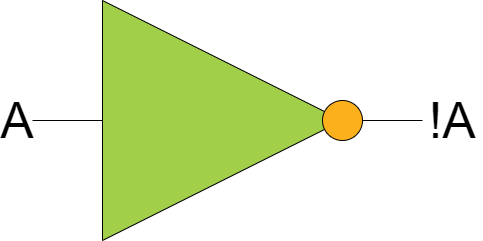
\includegraphics[height=1in]{digital_logic/NOT_gate.png}
        \caption[NOT Gate]{Visual representation of the NOT logical operation with one input and one output.}
    \end{figure}

    \pagelayout{wide} % Remove margins

    \begin{example}[Basic Logic Gates 1] \label{ex:basic-logic-gates-1}
        Let's practice the basic logic gates.
        We will consider a scenario with four inputs and we only want the logical output to be true when inputs A and B and (C or D) are true.
        We can set this up as the expression:
        \begin{equation*}
            (A \cdot B) + (C + D)
        \end{equation*}

        We will then establish the truth table as:
        \begin{center}
            \begin{tabular}{c c c c | c}
                \toprule
                Input D & Input C & Input B & Input A & Output \\
                \midrule
                    0    &    0     &    0     &    0     &    0    \\
                    0    &    0     &    0     &    1     &    0    \\
                    0    &    0     &    1     &    0     &    0    \\
                    0    &    0     &    1     &    1     &    0    \\
                    0    &    1     &    0     &    0     &    0    \\
                    0    &    1     &    0     &    1     &    0    \\
                    0    &    1     &    1     &    0     &    0    \\
                    0    &    1     &    1     &    1     &    1    \\
                    1    &    0     &    0     &    0     &    0    \\
                    1    &    0     &    0     &    1     &    0    \\
                    1    &    0     &    1     &    0     &    0    \\
                    1    &    0     &    1     &    1     &    1    \\
                    1    &    1     &    0     &    0     &    0    \\
                    1    &    1     &    0     &    1     &    0    \\
                    1    &    1     &    1     &    0     &    0    \\
                    1    &    1     &    1     &    1     &    1    \\
                \bottomrule
            \end{tabular}
        \end{center}
        Here, we can easily see that there are 3 input sets that will allow a logical true output in our scenario.

        Next, we can create a visual representation of this scenario:
        \begin{center}
            
\includegraphics[height=2.5in]{digital_logic/BasicGatesEx1.png}
        \end{center}

        While the required input set to get a logical true output is not obvious, it is a little easier to understand the "logic flow" through our scenario and we can test different input ideas and comprehend what is occurring a little easier.

        % \todo{Insert Arduino example!}
    \end{example}

    \begin{example}[Basic Logic Gates 2] \label{ex:basic-logic-gates-2}
        In this scenario, we are going to add a NOT gate and change the output conditions.
        Here we are looking for A and B or not (C or D).
        As before, we set up the scenario as the expression:
        \begin{equation*}
            A \cdot B + \overline{(C + D)}
        \end{equation*}

        We can also build the truth table:
        \begin{center}
            \begin{tabular}{c c c c | c}
                \toprule
                Input D & Input C & Input B & Input A & Output \\
                \midrule
                    0    &    0     &    0     &    0     &    1    \\
                    0    &    0     &    0     &    1     &    1    \\
                    0    &    0     &    1     &    0     &    1    \\
                    0    &    0     &    1     &    1     &    1    \\
                    0    &    1     &    0     &    0     &    0    \\
                    0    &    1     &    0     &    1     &    0    \\
                    0    &    1     &    1     &    0     &    0    \\
                    0    &    1     &    1     &    1     &    1    \\
                    1    &    0     &    0     &    0     &    0    \\
                    1    &    0     &    0     &    1     &    0    \\
                    1    &    0     &    1     &    0     &    0    \\
                    1    &    0     &    1     &    1     &    1    \\
                    1    &    1     &    0     &    0     &    0    \\
                    1    &    1     &    0     &    1     &    0    \\
                    1    &    1     &    1     &    0     &    0    \\
                    1    &    1     &    1     &    1     &    1    \\
                \bottomrule
            \end{tabular}
        \end{center}
        We can see from the table that we have several more conditions that will result in a true output from our expression!

        If we create a diagram of this scenario, we get the following:
        \begin{center}
            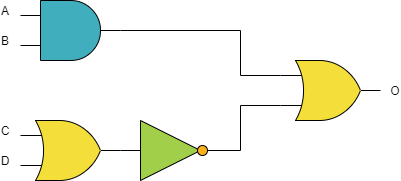
\includegraphics[height=2.5in]{digital_logic/BasicGatesEx2.png}
        \end{center}
    \end{example}

    \pagebreak

    \subsubsection*{Arduino Example: Basic Logic Gates}
        Let's practically demonstrate the circuit found in Example \ref{ex:basic-logic-gates-2} using your Arduino Kit!
        
        You will need:
        \begin{itemize}
            \item 4 Buttons
            \item 10 Male-to-Male jumper wires
            \item 1 220-$\Omega$ resistor
            \item 1 Red LED
        \end{itemize}

        Connect these components together in the following circuit:
        \begin{center}
            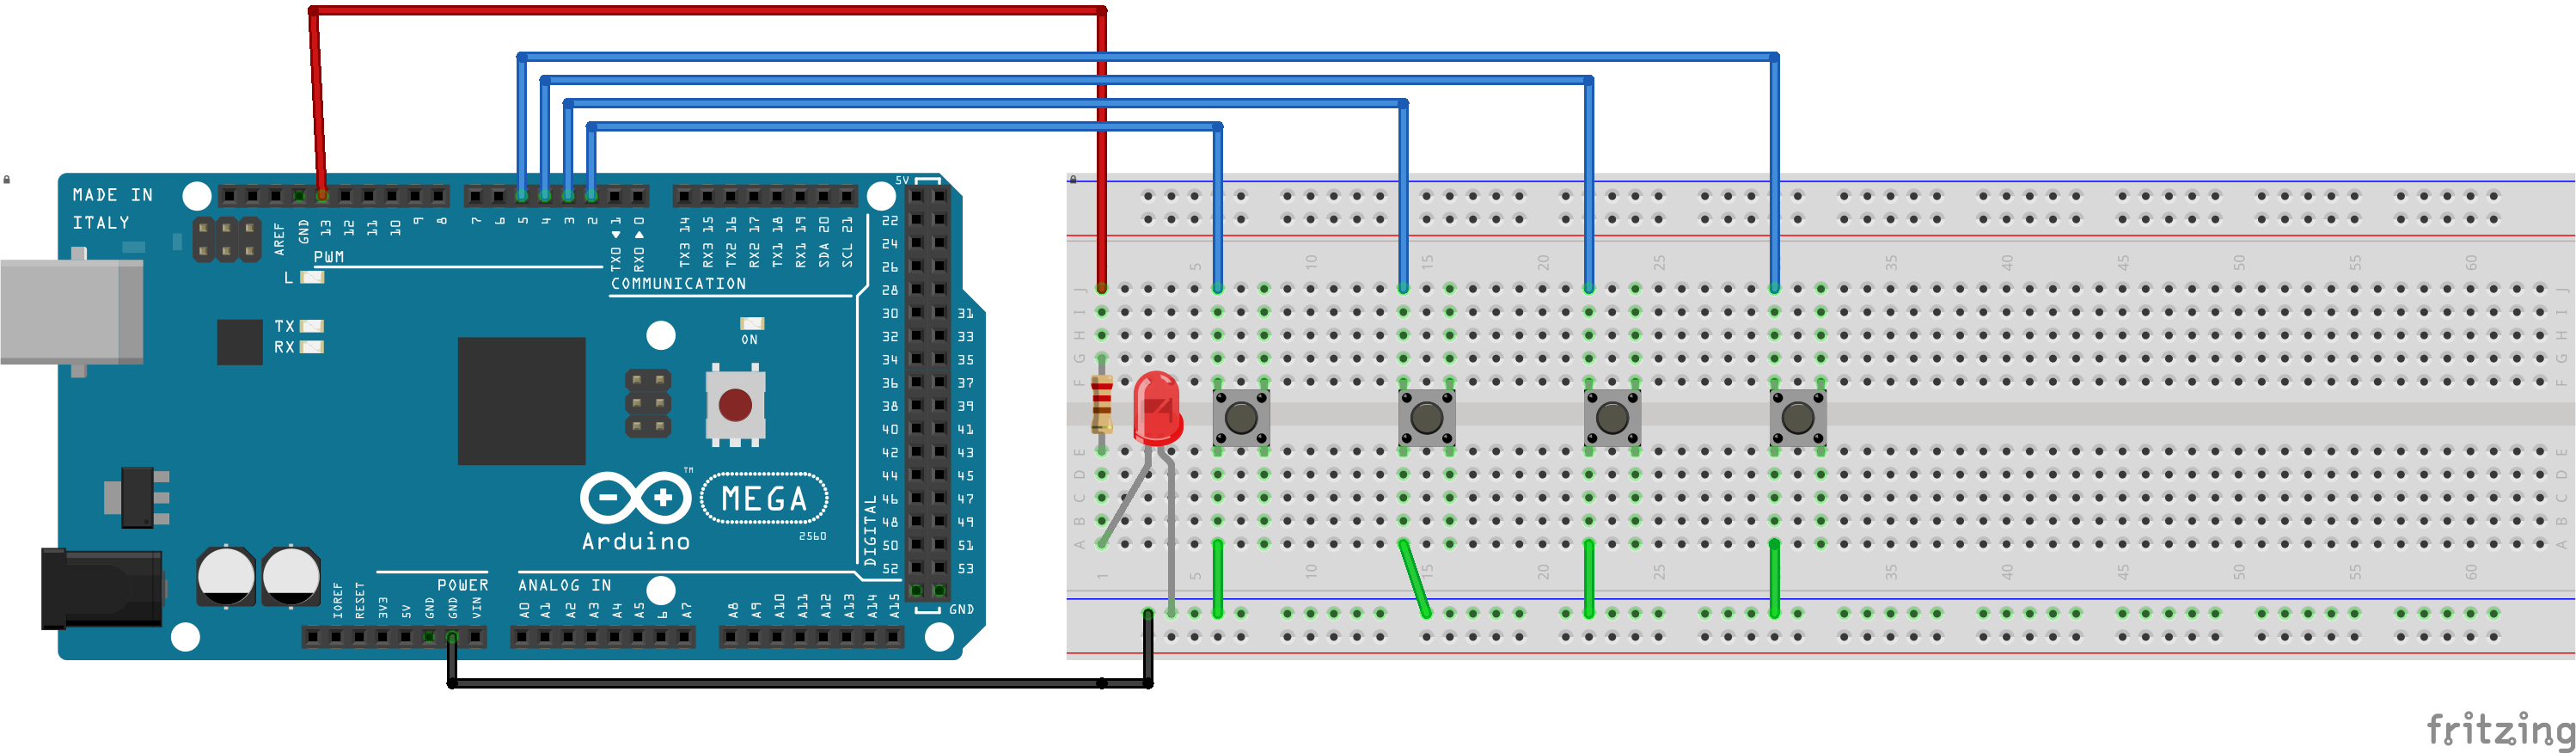
\includegraphics[]{examples/logic_gates_2_sch.png}
        \end{center}

        Then, we will use the following code to turn on or off the LED according to our button inputs.

        \lstinputlisting[language=C++, firstline=13]{../../src/examples/222-basic_logic_gates_2/222-basic_logic_gates_2.ino}

        Let's break down this code to understand what is occurring.
        First, we define the input pins for our four input buttons: A, B, C, and D.
        The C++ pre-processor command \lstinline[language=C++]{#define} essentially substitutes all calls of the variable name with the value we define in the second parameter.
        Ergo, whenever we have \lstinline[language=C++]{A} passed as a variable, the code will automatically substitute it with the value 2.
        We also create an array of all these pin numbers so we can more easily initialize them later.

        \lstinputlisting[language=C++, linerange={13-20}]{../../src/examples/222-basic_logic_gates_2/222-basic_logic_gates_2.ino}

        Then, we can define \lstinline[language=C++]{setup()} which is the first function the Arduino will call when it boots up.
        Any code that needs to be initialized first needs to be included within this function!
        Here, we have a simple for-loop that iterates through the pin array we defined earlier to initialize them all as \lstinline[language=C++]{INPUT_PULLUP}.
        This particular mode means the Arduino is able to take digital input signals on this pins and pull up these inputs to 5V using internal resistors.
        When we press a button, the pins are pulled low, giving a clear distinction between not pressed and pressed.
        We also set the builtin LED pin to an output so we can turn it on or off.

        \lstinputlisting[language=C++, linerange={22-28}]{../../src/examples/222-basic_logic_gates_2/222-basic_logic_gates_2.ino}

        This finally brings us to \lstinline[language=C++]{loop()} where we implement the actual digital logic.
        We first encounter the if-statement that is our logical expression for this example.
        It is important to note that here, \lstinline[language=C++]{&} is the bitwise AND operator, \lstinline[language=C++]{|} is the bitwise OR operator, and the \lstinline[language=C++]{!} is the bang or bitwise INVERT operator.
        Since this circuit is an active-low configuration, we must invert the readings from the input pins hence \lstinline[language=C++]{!digitalRead(A)}.
        If our logical expression is found to be true, we turn the LED on; otherwise, we turn it off using \lstinline[language=C++]{digitalWrite(LED_BUILTIN, HIGH/LOW)}.
        We then implement a delay of 125 milliseconds which is useful for debouncing the button inputs.

        \lstinputlisting[language=C++, linerange={30-36}]{../../src/examples/222-basic_logic_gates_2/222-basic_logic_gates_2.ino}

    \pagelayout{margin} % Restore margins

    \subsection{Combination Logical Operators}
    As we can see from the previous example, we can combine gates together to change their logical outputs accordingly.
    Adding a NOT gate to the first OR gate gave several more conditions that would make the system output a logical true value.
    However, it can be unnecessarily clumsy to draw a gate immediately followed by a NOT gate, so we can combine them together into a single gate.

    \paragraph*{The NAND operator} is a combination NOT and AND (NOT-AND, NAND) operation. 
    This means the operation outputs a logical true value only when both input 1 \textit{and} input 2 are \textit{not} true.
    \marginnote{For you computer storage afficionados out there, NAND flash memory is one of the predominant architectures for high speed, solid state drives.}
    This can be represented by the expression and truth table below:
    \begin{equation*}
        \overline{(A \cdot B)}
    \end{equation*}

    \begin{table}[h!]
        \labtab{nand_truth_table}
        \begin{tabular}{c c | c}
            \toprule
            $A$ & $B$ & $\overline{(A \cdot B)}$  \\
            \midrule
             0  &  0  &    1    \\
             0  &  1  &    1    \\
             1  &  0  &    1    \\
             1  &  1  &    0    \\
            \bottomrule
        \end{tabular}
    \end{table}

    This gate is graphically represented by the symbol. 
    As you can see, the NAND gate is distinguished from its former identity by the circle at the front of the gate.
    You may also notice that this is the same circle present at the tip of the NOT gate, clearly relating the two.
    \begin{figure}[h!]
        \labfig{nand_gate}
        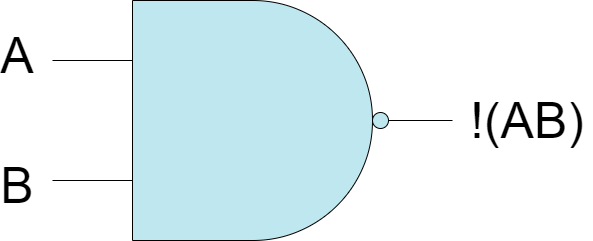
\includegraphics[height=1in]{digital_logic/NAND_gate.png}
        \caption[NAND Gate]{Visual representation of the NAND logical operation with two inputs and one inverted output.}
    \end{figure}

    \paragraph*{The NOR gate} is a combination NOT and OR (NOT-OR, NOR) operation.
    The bottom symbols in Example \ref{ex:basic-logic-gates-2} can be combined into this single operation to achieve the same effect in a more space-efficient manner.
    This gate has a similar equation to its predecessor, looking like:
    \begin{equation*}
        \overline{(A + B)}
    \end{equation*}

    It is represented by the truth table:
    \begin{table}[h!]
        \labtab{nand_truth_table}
        \begin{tabular}{c c | c}
            \toprule
            $A$ & $B$ & $\overline{(A + B)}$  \\
            \midrule
             0  &  0  &    1    \\
             0  &  1  &    0    \\
             1  &  0  &    0    \\
             1  &  1  &    0    \\
            \bottomrule
        \end{tabular}
    \end{table}

    And the graphical representation below. 
    Again, notice how the only distinguishing factor between a NOR and OR gate is the circle at the tip of the gate.
    \begin{figure}[h!]
        \labfig{nor_gate}
        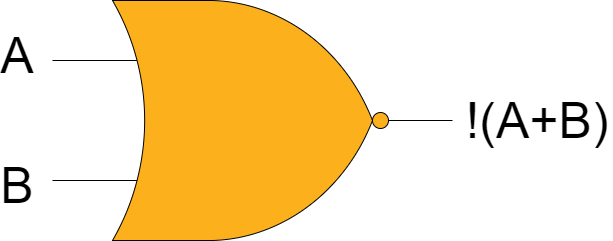
\includegraphics[height=1in]{digital_logic/NOR_gate.png}
        \caption[NOR Gate]{Visual representation of the NOR logical operation with two inputs and one inverted output.}
    \end{figure}

    \subsection{Advanced Logical Operators}
    Sometimes it is desirable to have some more limited conditions in which an operation will output a logical true.
    
    \paragraph*{The exclusive OR operation} is an operation that only outputs a logical true value when both inputs are different and not the same.
    This gate is represented by the expression:
    \begin{equation*}
        A \oplus B
    \end{equation*}

    This operation can also be shown by the truth table and gate visualization below:
    \begin{table}[h!]
        \labtab{xor_truth_table}
        \begin{tabular}{c c | c}
            \toprule
            $A$ & $B$ & $(A \oplus B)$  \\
            \midrule
             0  &  0  &    0    \\
             
             0  &  1  &    1    \\
             1  &  0  &    1    \\
             1  &  1  &    0    \\
            \bottomrule
        \end{tabular}
        \caption[XOR Gate Truth Table]{The truth table for the XOR gate.}
    \end{table}

    As we can see from the truth table, this operation can be best explained as "\textit{either or, but never both}"

    \begin{figure}[h!]
        \labfig{xor_gate}
        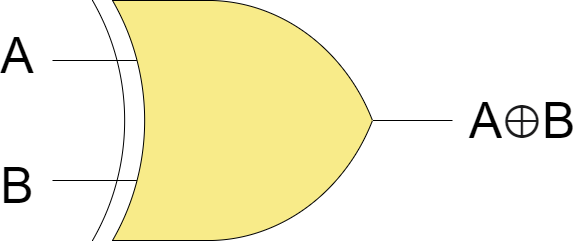
\includegraphics[height=1in]{digital_logic/XOR_gate.png}
        \caption[NOR Gate]{Visual representation of the NOR logical operation with two inputs and one output.}
    \end{figure}

    Note that the visual gate for the exclusive OR is differentiated from its basic counterpart by the additional arc at the back of the gate.

    \paragraph*{The XNOR operation} is just like previous combination operations where we combine the XOR operation with a NOT operation.
    This changes the input requirements for a logical true output to both inputs have to be the same, rather than they have to be different.
    This operation is created by combining multiple operations ike so:
    \begin{equation*}
        \overline{(A+B)} \cdot (A \cdot B)
    \end{equation*}
    And again, these complex combinations can be simplified by adding the $\oplus$ operator an negating it:
    \begin{equation*}
        \overline{(A \oplus B)}
    \end{equation*}

    This results in a truth table and graphical representation shown below:
    \begin{table}[h!]
        \labtab{xnor_truth_table}
        \begin{tabular}{c c | c}
            \toprule
            $A$ & $B$ & $\overline{(A \oplus B)}$  \\
            \midrule
             0  &  0  &    1    \\
             0  &  1  &    0    \\
             1  &  0  &    0    \\
             1  &  1  &    1    \\
            \bottomrule
        \end{tabular}
    \end{table}

    \begin{figure}[h!]
        \labfig{xnor_gate}
        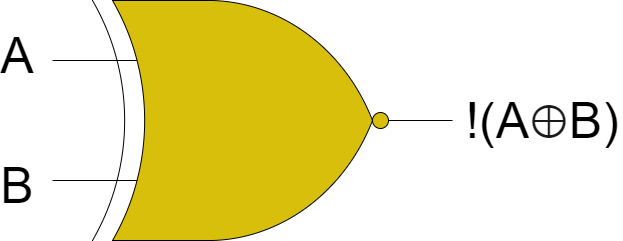
\includegraphics[height=1in]{digital_logic/XNOR_gate.png}
        \caption[XNOR Gate]{Visual representation of the XNOR logical operation with two inputs and one inverted output.}
    \end{figure}

\section{Boolean Algebra}
Boolean algebra can be sed to formalize expressions for logic states.
For these expressions, $A$ and $B$ are binary logical values, meaning they represent either a logical '1' or logical '0'.
$Q$ is representative of the logical output, again either a '1' or '0'.
Recall the following basic logical operations, multiplication denotes the AND operation, addition denotes the OR operation:
\begin{equation*}
    A \cdot A = A, A + A = A, A + \overline{A} = 1, A \cdot \overline{A} = 0, \overline{\overline{A}} = A
\end{equation*}

Using these basic definitions, we can define all of the logic gates described above as:

\begin{itemize}
    \item [AND: ]{$Q = A \cdot B$}
    \item [OR: ]{$Q = A + B$}
    \item [NOT: ]{$Q = \overline{A}$}
    \item [NAND: ]{$Q = \overline{A \cdot B}$}
    \item [NOR: ]{$Q = \overline{A + B}$}
    \item [XOR: ]{$Q = A \oplus B$}
    \item [XNOR:]{$Q = \overline{A \oplus B}$}
\end{itemize}

\begin{example}[Logic Gate Equivalency]
    In this example, we will be breaking down the XOR gate into it's composite boolean algebra expressions and logic gates.
    From Table \ref{tab:xor_truth_table} we can see this gate can be represented by the boolean algebra equation:
    
    \begin{equation*}
        Q = A \cdot \overline{B} + \overline{A} \cdot B
    \end{equation*}
    
    This garners the logic gate equality shown below:

    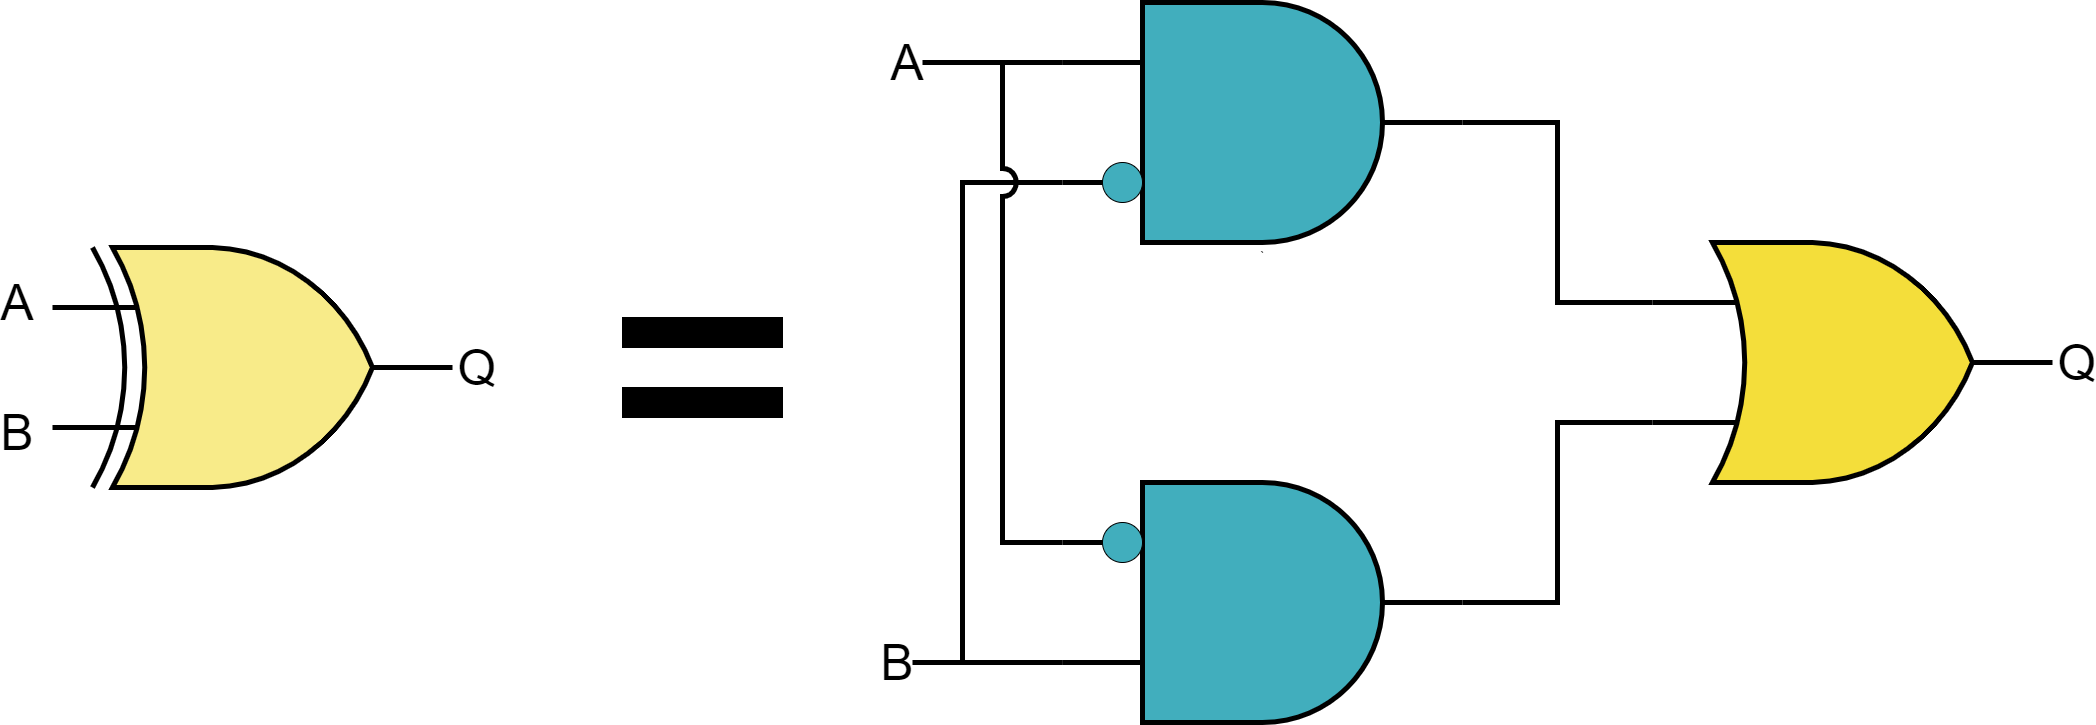
\includegraphics[height=3.5in]{digital_logic/XORGateBreakdown.png}
\end{example}

    \subsection[]{Logical Optimization}
    It is possible to represent any logical problem using an expression containing the appropriate order of AND and OR operations.
    However, for arbitrary truth tables and problems, this can create a lengthy process that is cumbersome, hard to write and follow, and can lead to extensive errors.
    This expression can also be needlessly inefficient and computationally expensive for calculators.
    Therefore, we can implement some strategies to reduce the computational load and optimize an arbitrary expression so we can improve computational efficiency and performance.

    For this process, two methods can be used: algebraic optimization and Karnaugh mapping.
    The former can be done by hand for relatively simple problems, or by a computer analysis when there are a large number of binary inputs.
    The latter is most commonly done by hand and drastically reduces the size of a truth table.
    This can make the logical problem easier to understand and represent.
    However, this method is limited to a maximum of four binary inputs.

    Let's examine a problem where we are given the arbitrary truth table shown in Table \ref{tab:optimize_table}.

    \begin{table}
        \labtab{optimize_table}
        \begin{tabular}{c c c c | c}
            \toprule
            Input D & Input C & Input B & Input A & Output \\
            \midrule
                0    &    0     &    0     &    0     &    1    \\
                0    &    0     &    0     &    1     &    0    \\
                0    &    0     &    1     &    0     &    0    \\
                0    &    0     &    1     &    1     &    1    \\
                0    &    1     &    0     &    0     &    0    \\
                0    &    1     &    0     &    1     &    0    \\
                0    &    1     &    1     &    0     &    0    \\
                0    &    1     &    1     &    1     &    0    \\
                1    &    0     &    0     &    0     &    1    \\
                1    &    0     &    0     &    1     &    1    \\
                1    &    0     &    1     &    0     &    1    \\
                1    &    0     &    1     &    1     &    1    \\
                1    &    1     &    0     &    0     &    1    \\
                1    &    1     &    0     &    1     &    0    \\
                1    &    1     &    1     &    0     &    0    \\
                1    &    1     &    1     &    1     &    1    \\
            \bottomrule
        \end{tabular}
        \caption[Optimization Truth Table]{An arbitrary truth table ripe for optimization}
    \end{table}

    We can begin exploring the algebraic optimization by writing the algebraic expression for the true values of the table:
    
    \begin{equation*}
        Q = \overline{ABCD} + C + A + AC + AB + ABD + ABC + ABCD 
    \end{equation*}

    Using algebraic simplification:

    \begin{align}
        Q &= \cancel{\overline{ABCD}} + \cancel{ABCD} + CD + A(1 + C + B + BD + \cancel{BC}) \nonumber \\
          &= C + A(1 + C + B + BD) \nonumber \\
          &= C + A + \cancel{AC} + AB + BD \nonumber \\
        Q &= C + A + AB + ABD \nonumber
    \end{align}

    \marginnote[-1.5in]{Here, you will notice some AND expressions have been cancelled out (re: $BC$ and $AC$).
    This has occurred because the expressions $ B + C + BC$ and $A + C + AC$ simplify down to the first OR operation.
    Let's explore this by drawing out the truth table for these expressions: \\
    \begin{tabular}{c c | c}
        \toprule
        $B$ & $C$ & $B+C+BC$ \\
        \midrule
        0 & 0 & 0 \\
        0 & 1 & 1 \\
        1 & 0 & 1 \\
        1 & 1 & 1 \\
        \bottomrule
    \end{tabular} \\
    You will notice that this truth table is the exact same for the OR gate (Table \ref{tab:or_truth_table}) and therefore proves the simplification and cancellation of the AND operation.
    }

    This expression is complicated and would require three OR gates, and three AND gates to represent.
    Let's see if we can simplify this using a Karnaugh map.

    \paragraph*{Karnaugh Maps} or K-maps, are condensed representations of truth tables that combine up to four distinct inputs into a two-dimensional table.
    These not only condense truth tables into a simpler form for easier understanding, but they can simultaneously simplify the algebraic expression for the truth table.
    K-Maps have a special property where if any logical true outputs that are grouped together in powers of 2 can be combined into a simpler AND operation.

    For the example found in Table \ref{tab:optimize_table}, the corresponding K-Map would be:

    \begin{karnaugh-map}(label=corner)[4][4][1][$B$][$A$][$D$][$C$]
        \manualterms{1,0,1,0,0,0,0,0,1,0,1,0,1,1,1,1}
        \implicant{12}{14}
        \implicantcorner
    \end{karnaugh-map}

    The highlighted groupings mean the truth table from before can be represented by the algebraic expression:

    \begin{equation*}
        Q = AB + \overline{BD}
    \end{equation*}

    \pagelayout{wide} % Remove margins

    \begin{example}[Applied Logic Gate Simplification] \label{ex:advanced-logic-gates}
        For this example, we will be combining everything we have learned through this section into a single problem.
        We will start with the logic gate diagram shown below:
        
        \begin{center}
            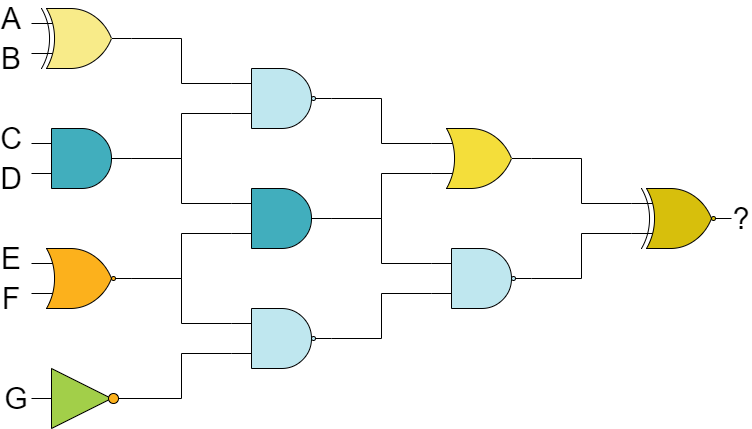
\includegraphics[height=2.5in]{digital_logic/AdvancedGatesEx.png}
        \end{center}

        We can represent these gates with the expression:

        \begin{equation*}
            Q = (A+B)C \oplus \overline{D}
        \end{equation*}

        Which expands to:

        \begin{equation*}
            Q = \left((AC + BC)\overline{D}\right) + \left((\overline{AB} + \overline{C})D\right)
        \end{equation*}

        This expression is a little complicated and is not ideal to determine what inputs will result in our desired outputs.
        Therefore, we will construct a truth table to represent these logic gates so that we can directly check a given output with an expected output.

        \begin{center}
            \begin{tabular}{c c c c | c}
                \toprule
                Input D & Input C & Input B & Input A & Output \\
                \midrule
                    0    &    0     &    0     &    0     &    0    \\
                    0    &    0     &    0     &    1     &    1    \\
                    0    &    0     &    1     &    0     &    0    \\
                    0    &    0     &    1     &    1     &    0    \\
                    0    &    1     &    0     &    0     &    0    \\
                    0    &    1     &    0     &    1     &    1    \\
                    0    &    1     &    1     &    0     &    1    \\
                    0    &    1     &    1     &    1     &    0    \\
                    1    &    0     &    0     &    0     &    0    \\
                    1    &    0     &    0     &    1     &    1    \\
                    1    &    0     &    1     &    0     &    1    \\
                    1    &    0     &    1     &    1     &    0    \\
                    1    &    1     &    0     &    0     &    0    \\
                    1    &    1     &    0     &    1     &    1    \\
                    1    &    1     &    1     &    0     &    1    \\
                    1    &    1     &    1     &    1     &    0    \\
                \bottomrule
            \end{tabular}
        \end{center}

        Both the representative expression and truth table are a little large and inefficient.
        If we look at the representative expression, we will notice that it is difficult, if not impossible, to algebraically simplify by hand. 
        So, we will simplify the truth table with a Karnaugh map and determine the simplified algebraic expression from there.
        
        \begin{center}
            \begin{karnaugh-map}(label=corner)[4][4][1][$B$][$A$][$D$][$C$]
                \manualterms{0,0,0,0,1,1,1,1,0,1,1,1,0,0,0,0}
                \implicant{4}{6}
                \implicant{9}{11}
                \implicant{11}{10}
            \end{karnaugh-map}
        \end{center}

        From the K-map, we can simplify the algebraic expression for the logic diagram as:

        \begin{equation*}
            Q = \overline{C}D + BC\overline{D} + AC\overline{D}
        \end{equation*}

        This expression is the most basic form for the logic diagram and now we can check any arbitrary value of $A$, $B$, $C$, or $D$ without have to directly look it up in the truth table or run it through the logic diagram.
    \end{example}

    \pagelayout{margin} % Restore margins

\section[]{Registers and Memory}

% ===========================================
% Electrical Schematics
% Written by: Braidan Duffy
%
% Date: 07/18/2022
% Last Revision: 07/26/2022
% ============================================

\setchapterstyle{koa}
\chapter{Electrical Schematics}
\setchapterpreamble[u]{\margintoc}
\labch{electrical_schemcatics}

One of the key pieces of instrumentation design is the electrical schematic and Printed Circuit Board (PCB).

\section{Schematic Basics}
\todo{Set chapter image to a schematic OR paste a big image of a goo schematic somewhere on this page}
The electrical schematic is a key piece of documentation that communicates to engineers what the circuit is comprised of and how it will work.
All modern electronic devices have schematics of varying complexity and depth that describe how electrons flow from one piece to another and document what behaviors can be expected during operations.
To understand these documents is to understand how a product fundamentally works, and to understand how to make these documents well is a skill that needs to practiced and refined by reviewing schematics and having yours reviewed.
For now, we will go over the basics and give you a fundamental understanding of what the schematic entails and what most of the symbols you might encounter mean.
\section{Basic Notation}


\section{Component Symbols}
The core of the schematic are the 2D representations of the components in the design called, \emph{symbols}. 
There are a variety of symbols that all mean different things and can have slightly different meanings depending on the drawer and application.
The symbols covered henceforth are the standard-accepted versions so they should be what you see in most schematics you may encounter or be asked to work with or design.

    \subsection{Power Symbols} 
    Power symbols are the set of symbols that indicate where the electrical power is coming from, and where it is going.

        \subsubsection*{The Power Source Rail} 
        the power source rail is typically denoted by a vertical "T" or arrow as shown below, and can be labelled with 3V3,\sidenote{Sometimes, it is easier to use a letter to represent a decimal point. 
        In this case, 3V3 is 3.3 volts.}
        5V, VBAT, VBUS, or any other source name.

        \begin{figure}[h!]
            \labfig{power_rail_symbol}
            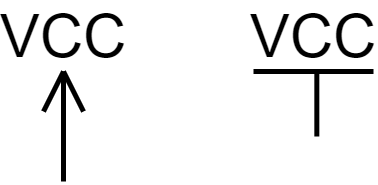
\includegraphics[height=1in]{electrical_schematics/power_rail_symbols.png}
            \caption[Power Rail Symbols]{Schematic symbols for power rails.
            The value label at the top can be any value like 3V3, 5V, etc.}
        \end{figure}

        \subsubsection*{The Power Sink Rail} 
        The power sink rail is the "ground" path from electrical energy will flow back to the negative terminal of the power supply. 
        It is typically represented by a vertical "$\perp$" or upside down tree as shown in \hl{FIGURE}.
        It should always be labelled "GND" with sometimes a prefix of "A" or "D" to denote a different analog or digital ground reference.

        \begin{figure}[h!]
            \labfig{power_sink_symbol}
            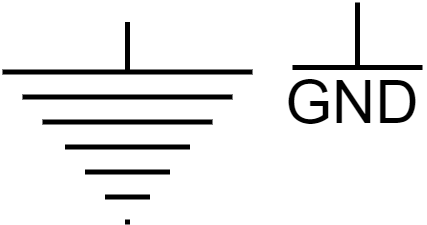
\includegraphics[height=1.25in]{electrical_schematics/ground_rail_symbols.png}
            \caption[Power Rail Symbols]{Schematic symbols for ground rails.}
        \end{figure}

        \subsubsection*{Power Supplies} are generally represented by a circle with a positive and negative input.
        In order to differentiate a DC supply and AC supply, we can use either a plus/minus or sine wave, respectively.
        Both of these symbols are represented in the figure below.

        \begin{figure}[h!]
            \labfig{power_source_symbol}
            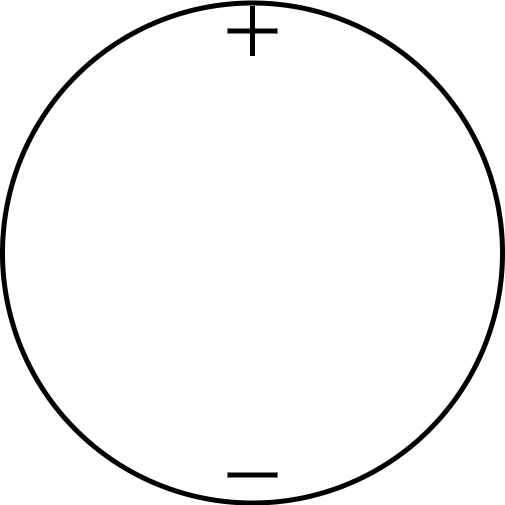
\includegraphics[height=1in]{electrical_schematics/DC_source_symbol.png}
            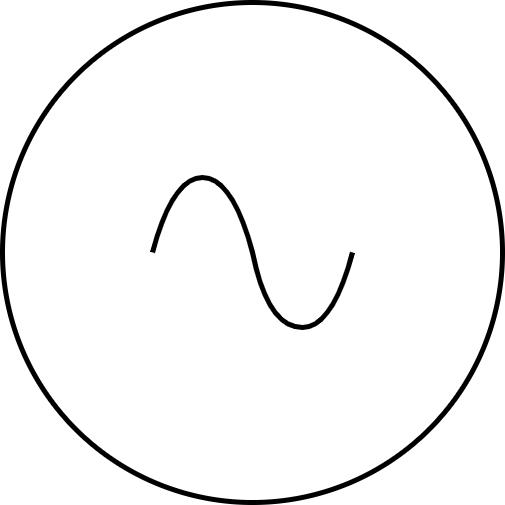
\includegraphics[height=1in]{electrical_schematics/AC_source_symbol.png}
            \caption[Source Symbols]{Schematic symbols for DC and AC power sources, respectively. 
            Notice how the AC power source uses a sinusoidal wave to differentiate it.}
        \end{figure}

        \paragraph*{The Battery} is a subset of DC power supply for embedded applications or circuits that will not have access to a general DC power supply.
        These components are meant to store a large amount of electrical charge for a long duration and be able to discharge it into a circuit to run it.
        Some batteries, like Lithium Ion batteries, are capable of being recharged using special integrated circuits and power supplies.
        Others, like alkaline batteries, are only usable once and must be disposed of properly when they are depleted.

    \begin{marginfigure}[-2in]
        \labfig{battery_real}
        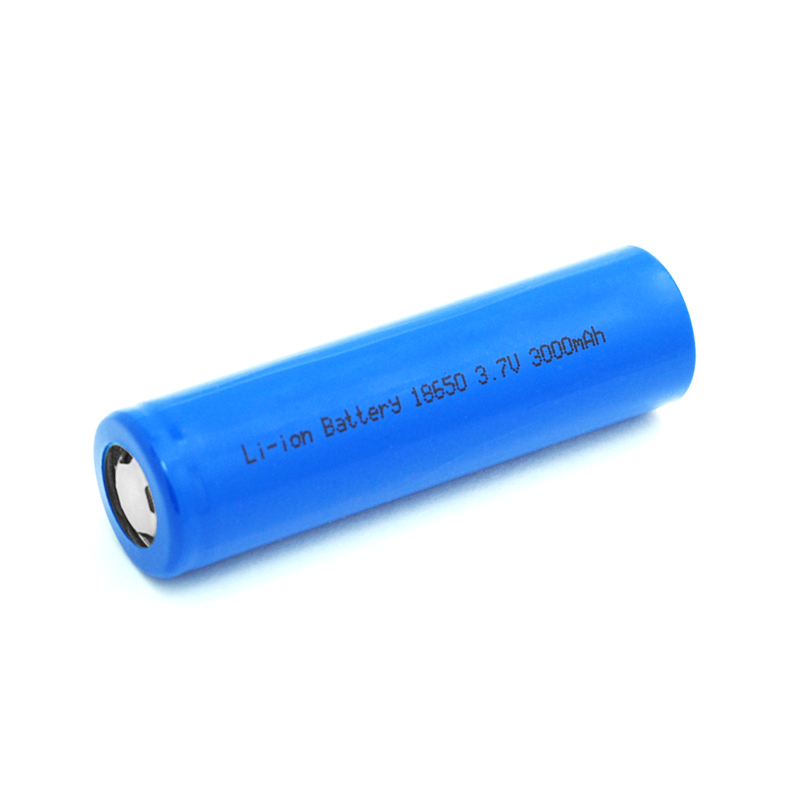
\includegraphics[]{electrical_schematics/battery.jpg}
        \caption[Chip Resistors]{18650 Li-ion battery. 
        Retrieved from \href{https://himaxelectronics.com/product-item/18650-3000mah-li-ion-battery-cell/}{Himax Electronics}}
    \end{marginfigure}

    \begin{figure}[h!]
        \labfig{battery_symbol}
        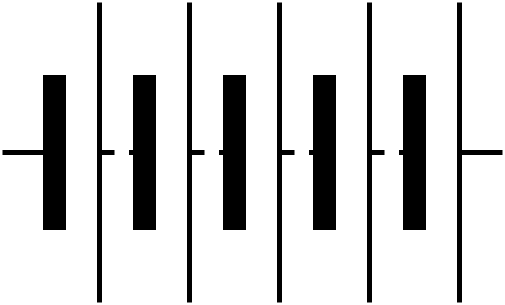
\includegraphics[height=1in]{electrical_schematics/battery_symbol.png}
        \caption[Resistor Symbols]{Schematic symbol for a battery. 
        The different sized lines that comprise the battery symbol represent the different plates that are within modern battery construction.}
    \end{figure}

    \subsection{Basic Components} 
    The following basic component symbols represent discreet components within an electrical circuit.
    Most of these components perform a single service within the circuit and must be used in conjunction with other basic parts to achieve an action.

        \subsubsection*{Resistors} 
        Resistors are components that resist the flow of current and can be used to dissipate energy, reduce voltage levels, or limit current going into other components.
        There are represented with a jagged line or box with "whiskers" as shown in the figure below.

        \begin{marginfigure}[-1in]
            \labfig{resistor_real}
            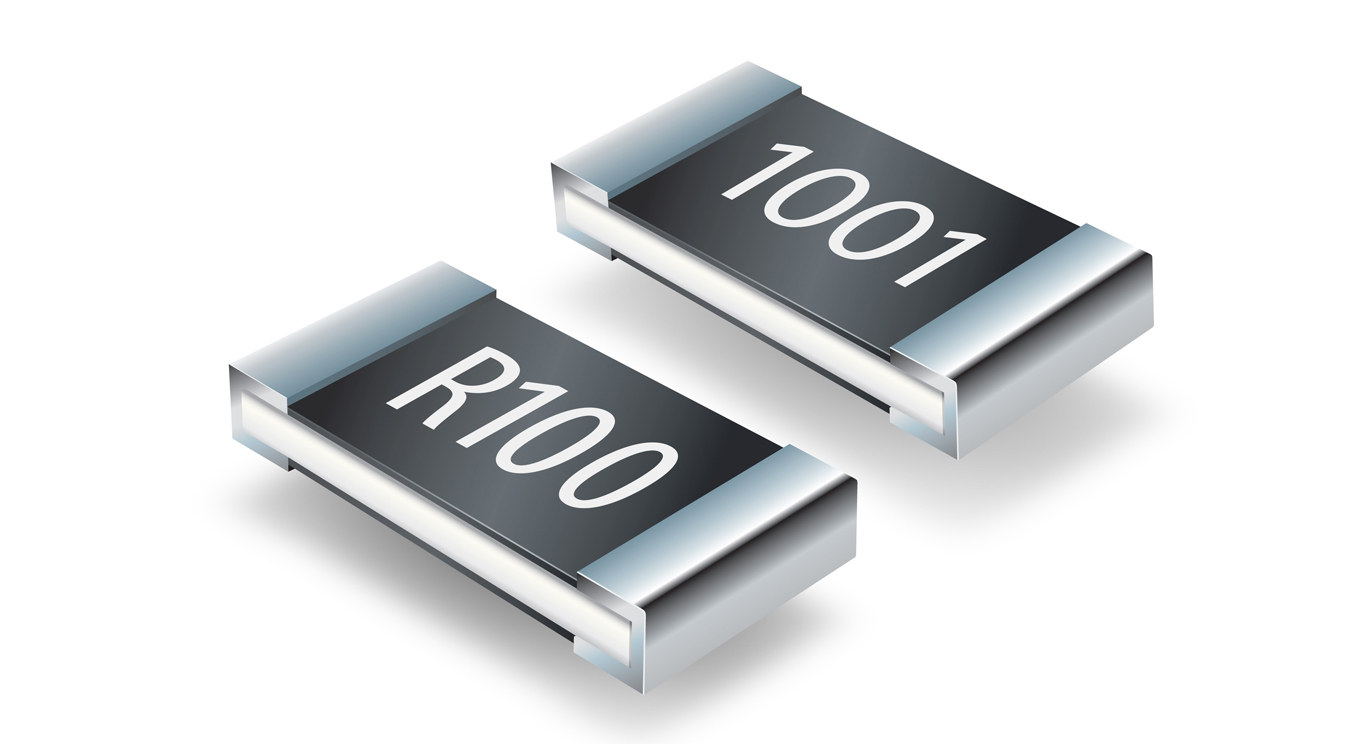
\includegraphics[]{electrical_schematics/chip_resistors.jpg}
            \caption[Chip Resistors]{Surface mount chip resistors. 
            Retrieved from \href{https://www.mpdigest.com/2018/01/24/thick-film-chip-resistors/}{MPDigest}}
        \end{marginfigure}

        \begin{figure}[h!]
            \labfig{resistor_symbol}
            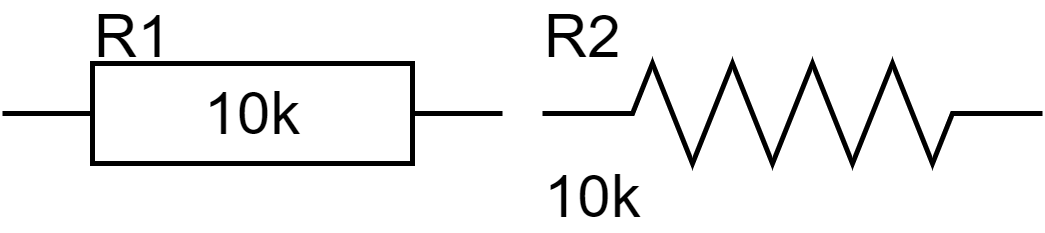
\includegraphics[width=4in]{electrical_schematics/resistors_symbols.png}
            \caption[Resistor Symbols]{Schematic symbols of resistors. 
            European standard is the left, US standard to the right.}
        \end{figure}

        \paragraph*{The Potentiometer} is a variable resistor that changes resistance depending on the position of "wiper" across a band of resistive material.
        Typically, these components are turned by human operators and can be used as an input to determine a variety of things, depending on application.

        \begin{marginfigure}[-1in]
            \labfig{potentiometer_real}
            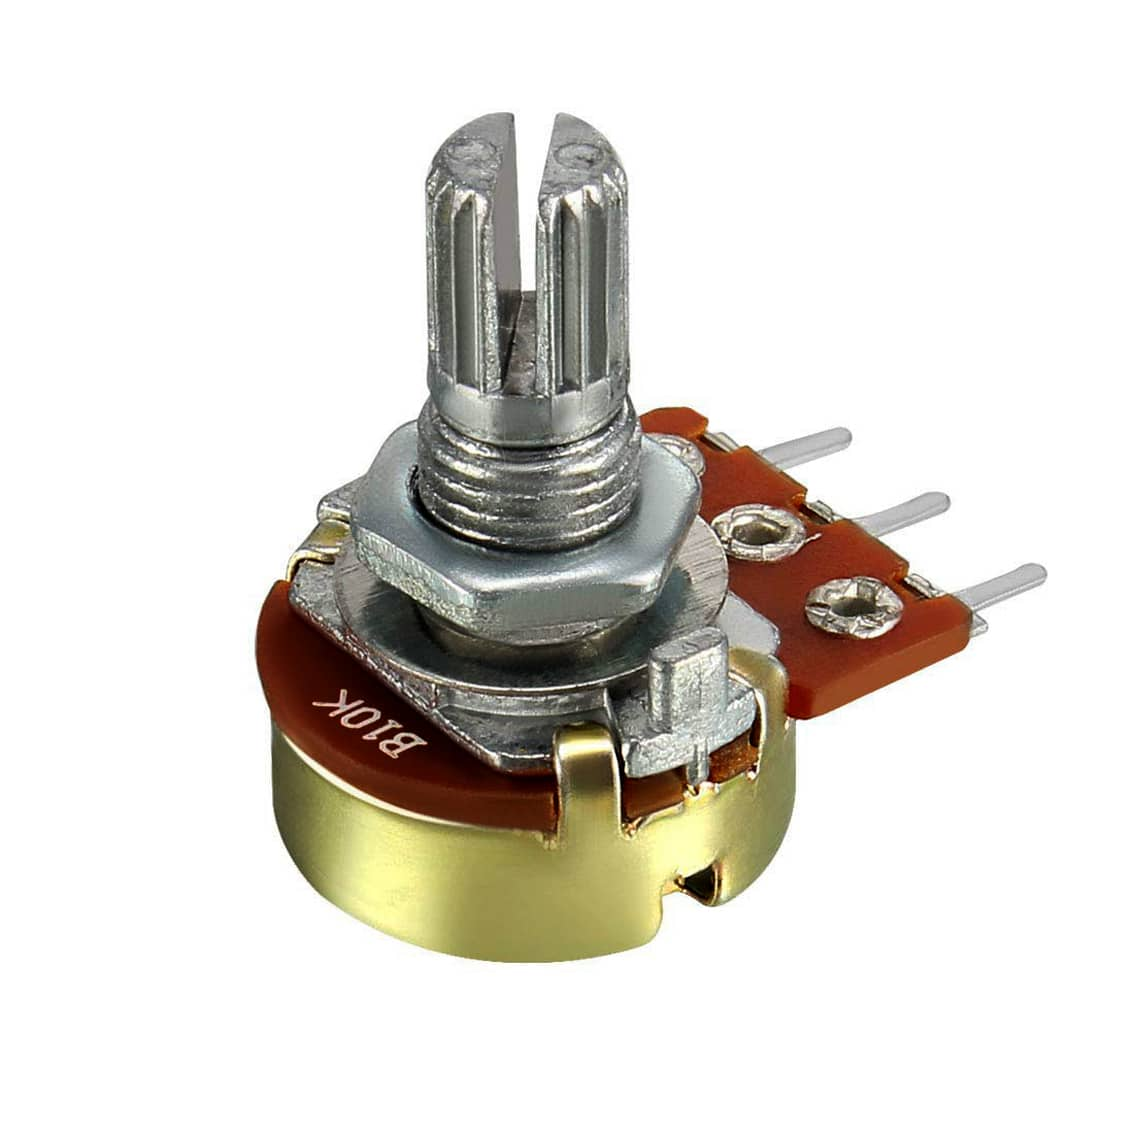
\includegraphics[height=1.5in]{electrical_schematics/potentiometer.jpg}
            \caption{Panel mount potentiometer.
            Retrieved from \href{https://www.phippselectronics.com/product/10k-potentiometer-panel-mount-breadboard-friendly-pack-of-2/}{Phipps Electronics}}
        \end{marginfigure}

        \begin{figure}[h!]
            \labfig{potentiometer_symbol}
            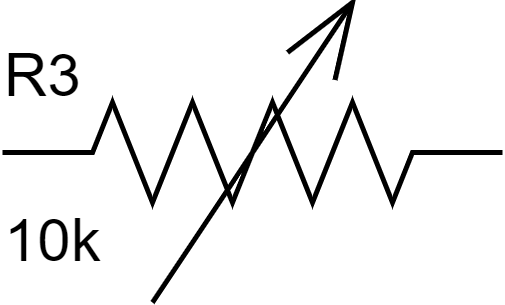
\includegraphics[height=1.5in]{electrical_schematics/potentiometer_symbol.png}
            \caption[Potentiometer Symbol]{Schematic symbols for potentiometers. Notice the arrow through the resistor to demark it from standard resistors. The value at the bottom is the maximum resistance.}
        \end{figure}

        \paragraph*{Photoresistor}
        The photoresistor is a variable resistor that changes resistance depending on the intensity of light interacting with it
        Typically, these components are used as basic light sensors that can be used for presence detection, sun tracking, or other light intensity measurement.

        \begin{marginfigure}[-1in]
            \labfig{photoresistor_real}
            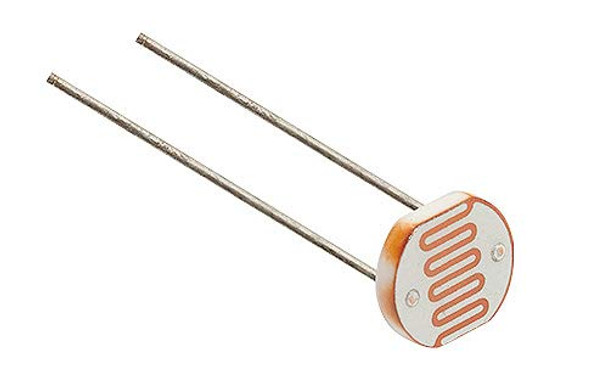
\includegraphics[]{electrical_schematics/photoresistor.jpg}
            \caption{LDR photoresistor.
            Retrieved from \href{https://www.pixelelectric.com/sensors/light-sound/light-color-sensor/5528-ldr-mini-photoresistor/}{Pixel Electric}}
        \end{marginfigure}

        \begin{figure}[h!]
            \labfig{potentiometer_symbol}
            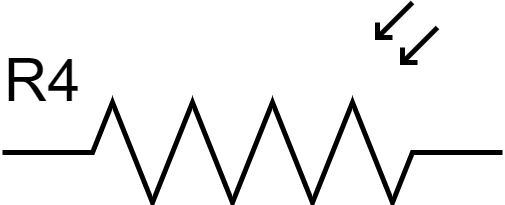
\includegraphics[height=1in]{electrical_schematics/photoresistor_symbol.png}
            \caption[Potentiometer Symbol]{Schematic symbols for photoresistors. The arrows pointed towards the resistor indicate its light dependency.}
        \end{figure}

        \subsubsection*{Capacitors}
        Capacitors are components that store and discharge electrical energy.
        They use parallel conducting plates isolated from each other with a dielectric that allows charges to build up on one face at a certain voltage, then discharge when at a lower voltage.
        This gives capacitors the ability to smooth ripples in voltage levels (called a decoupling).
        This is commonly used to decouple components from electrical noise upstream of their power supply, giving them a cleaner electrical input.
        Additionally, they can provide a high current energy source that has some advantages over traditional batteries.
        In most circuits, you will encounter ceramic capacitors (pictured to the side) that do not hold a log of charge, but work for most applications.
        These capacitors are bi-directional or non-polarized so they can be placed in any orientation on the schematic.

        \begin{marginfigure}[-2in]
            \labfig{capacitors_real}
            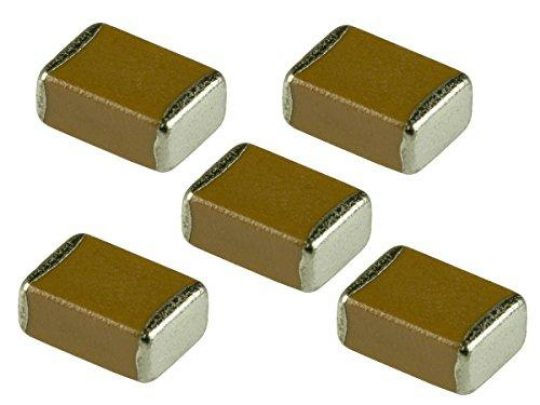
\includegraphics[]{electrical_schematics/capacitors.jpg}
            \caption{Chip ceramic capacitors.
            Retrieved from \href{https://universal-solder.ca/product/320-pcs-ultimate-smd-1206-ceramic-capacitors-kit-10pf-to-22uf/}{Universal Solder}}
        \end{marginfigure}

        \begin{figure}[h!]
            \labfig{capacitors_symbols}
            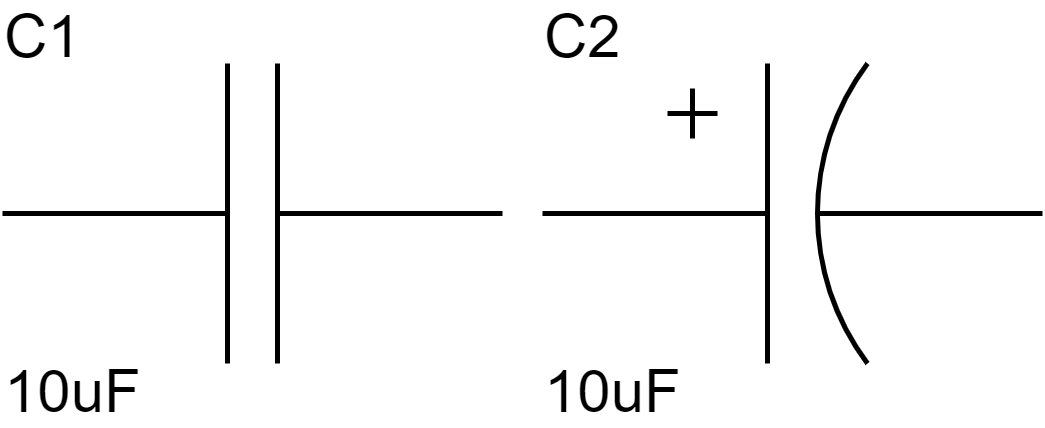
\includegraphics[height=1.5in]{electrical_schematics/capacitor_symbols.png}
            \caption[Potentiometer Symbol]{Schematic symbols for Capacitors. 
            On the left is the symbol for a non-polarized bi-directional capacitor.
            On the right is the symbol for an electrolytic or polarized capacitor.}
        \end{figure}

        \paragraph*{Electrolytic Capacitors} are polarized or uni-directional capacitors that use a liquid electrolyte compared to the ceramic ones used in non-polarized capacitors.
        These capacitors must be placed in a specific orientation otherwise they may become damaged and could explode!
        On electrical schematics, the negative terminal of these capacitors is denoted by a curved line, like shown above.
        Even though, you must closely pay attention to how the capacitor is orientated, the electrolytic capacitor provides a much high energy density compared to the ceramic capacitors, making them more suited for high power application.

        \begin{marginfigure}[-1.5in]
            \labfig{electro_capacitor}
            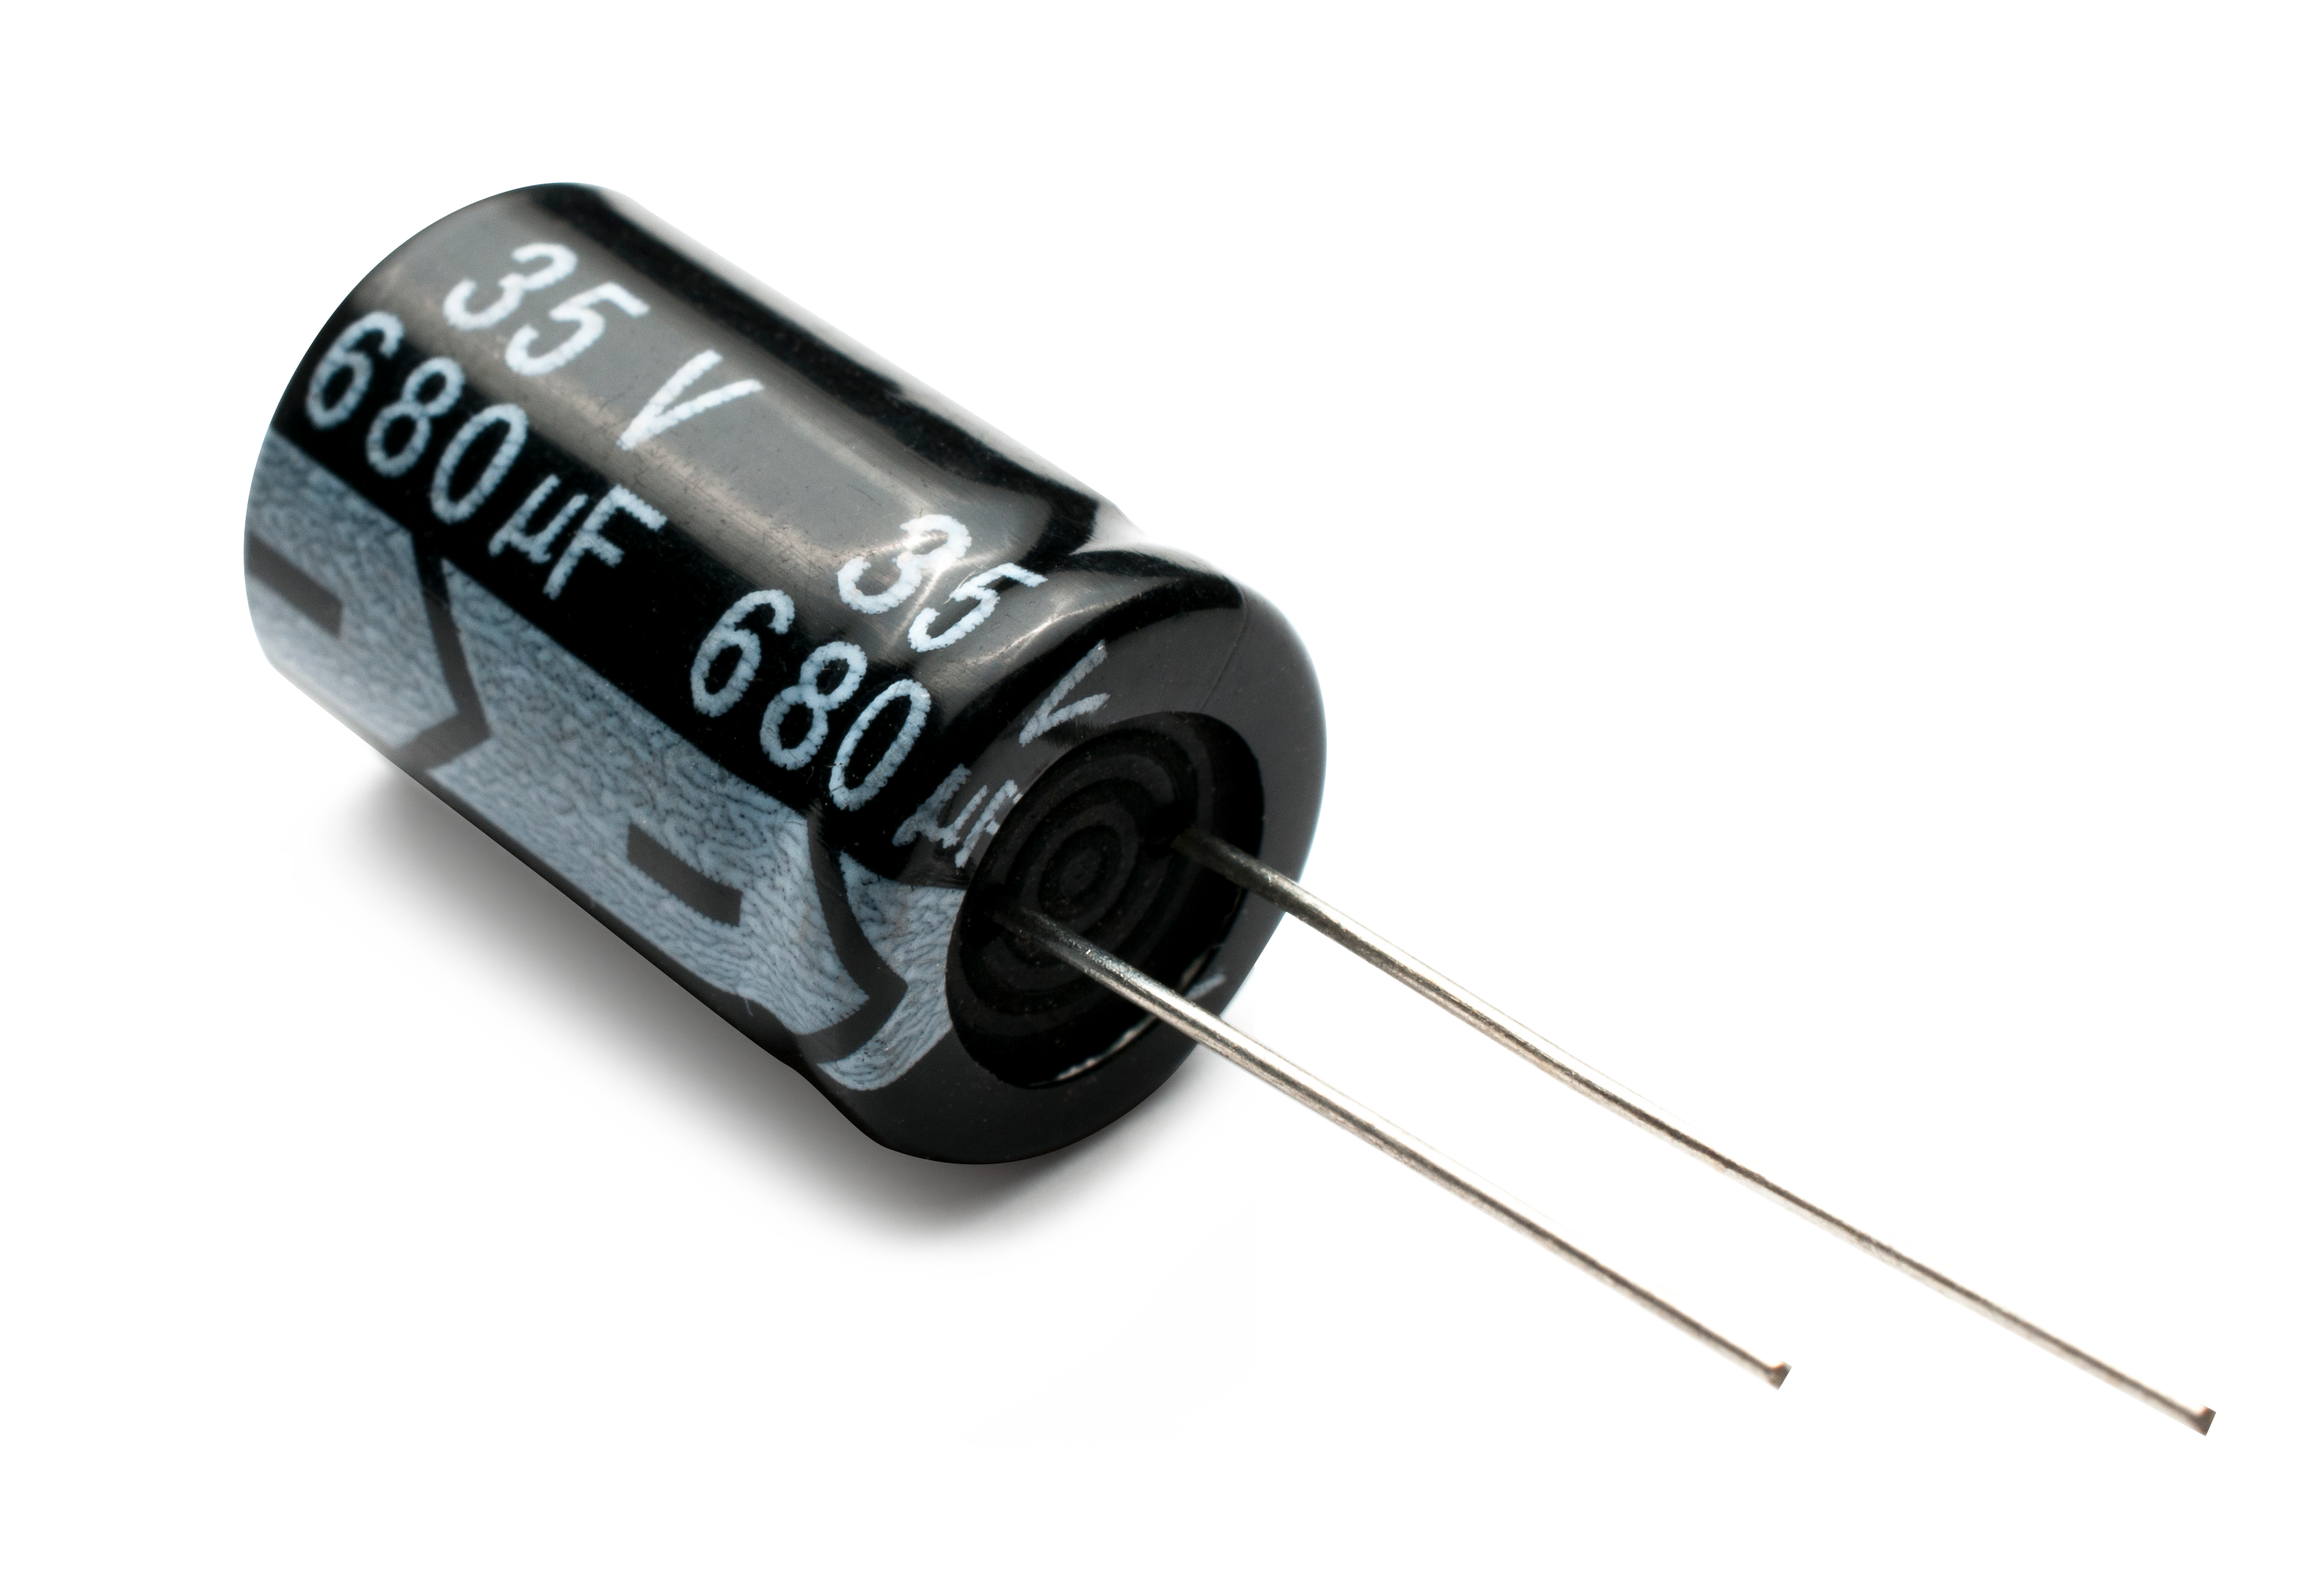
\includegraphics[]{electrical_schematics/electro_capacitor.png}
            \caption{Electrolytic capacitor.
            Notice the longer lead indicates the positive terminal and the negative terminal is clearly marked with a stripe on the casing.
            Retrieved from \href{https://www.srgllc.com/us/en/settlements/electronics/electrolytic-capacitors-indirect-purchaser}{SRG LLC}}
        \end{marginfigure}

        \subsubsection*{Inductors}
        Inductors are tiny electromagnetic that wind conducting wire around an iron or air core.
        When alternating electrical current is passed through the inductor, some of the energy is buffered in the magnetic field of the electromagnet. 
        You can think of them as electrical flywheels that store moving charge and can discharge it to maintain a more constant "flow".
        This makes inductors useful for resisting changes in current or acting as the analogue to capacitors in AC circuits.

        % \begin{marginfigure}[-1in]
        %     \labfig{inductor_real}
        %     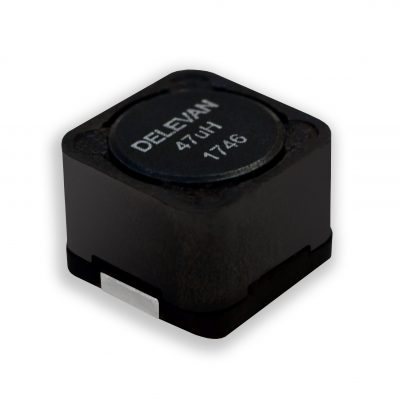
\includegraphics[]{electrical_schematics/inductor.jpeg}
        %     \caption{Surface mount inductor.
        %     Retrieved from \href{https://www.ept.ca/products/shielded-surface-mount-power-inductors-deliver-high-reliability/}{EP\&T}}
        % \end{marginfigure}

        \begin{figure}[h!]
            \labfig{inductor_symbol}
            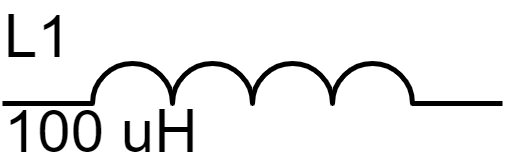
\includegraphics[height=1in]{electrical_schematics/inductor_symbol.png}
            \caption[Inductor Symbol]{Schematic symbol for inductors.}
        \end{figure}

        \subsubsection*{Diodes}
        Diodes are used to restrict current flow in a certain direction.
        This is accomplished using some electrochemical wizardry and comes at the cost of a little bit of voltage drop through the diode.
        But, the main property of the diode makes it invaluable for protecting circuits against reverse polarity, dissipating AC current, or even rectifying AC voltages into DC.

        \begin{marginfigure}[-1in]
            \labfig{diode_real}
            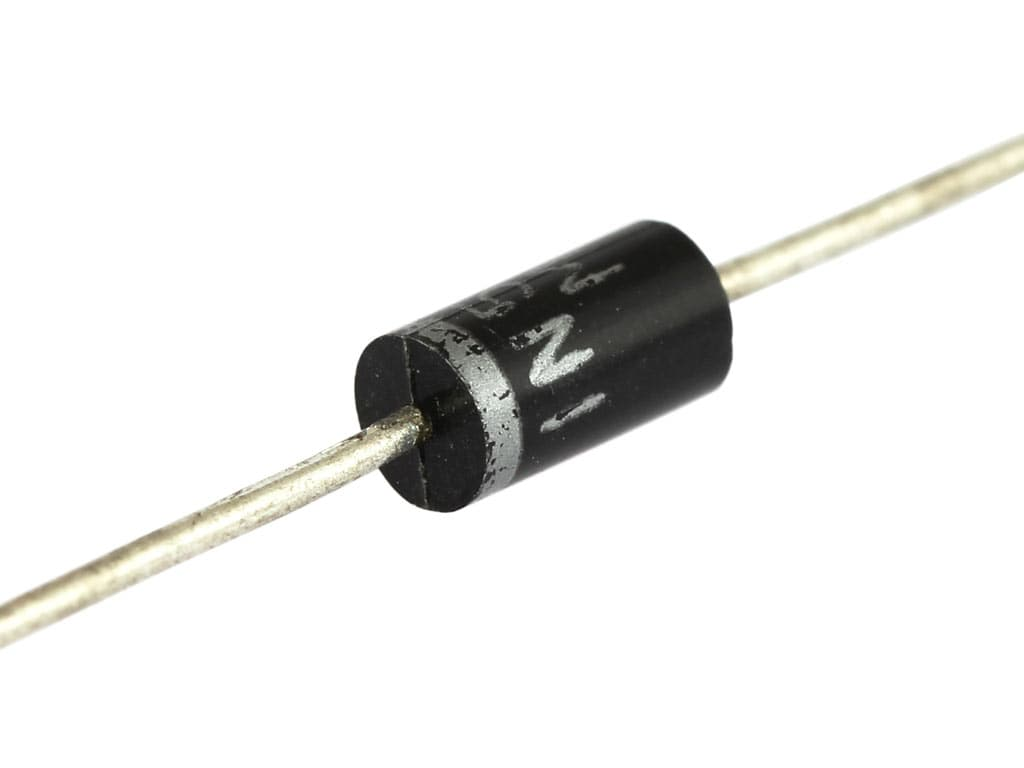
\includegraphics[]{electrical_schematics/diode.jpg}
            \caption{Through hole diode as commonly found in Arduino kits.
            Retrieved from \href{https://analyseameter.com/2016/03/diodes-types-operation-symbol-applications.html}{AnalyzeAMeter}}
        \end{marginfigure}

        \begin{figure}[h!]
            \labfig{diode_symbol}
            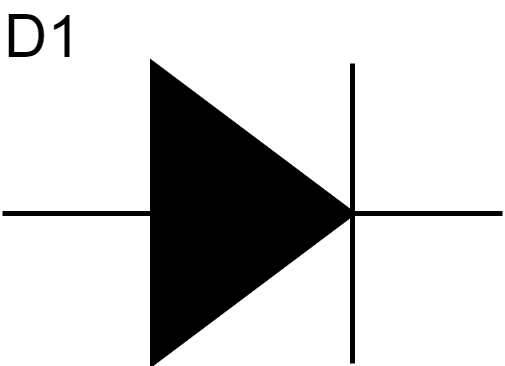
\includegraphics[height=1in]{electrical_schematics/diode_symbol.png}
            \caption[Diode Symbol]{Schematic symbol for diodes.}
        \end{figure}

        \paragraph*{Light Emitting Diodes (LEDs)} are diodes that siphon a little bit of electrical energy to emit photons at specific wavelengths.
        These components are ubiquitous in any application that requires a simple human interface such as light indicators, RGB gaming products, or flashlights.
        LEDs are smaller, easily scaled to almost any production scale, and more energy efficient compared to most other light sources in use today.

        \begin{figure}[h!]
            \labfig{led_symbol}
            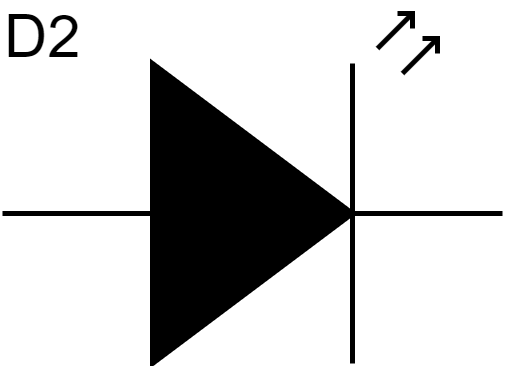
\includegraphics[height=1in]{electrical_schematics/led_symbol.png}
            \caption[LED Symbol]{Schematic symbol for light emitting diodes.}
        \end{figure}

        \paragraph*{Zener Diode} are special diodes that restricts the current flow direction up to a certain breakdown voltage.
        When that voltage is achieved, current is allowed to flow against the diode, without damaging it, making it useful in applications like circuit protection.

        \begin{figure}[h!]
            \labfig{zener_diode_symbol}
            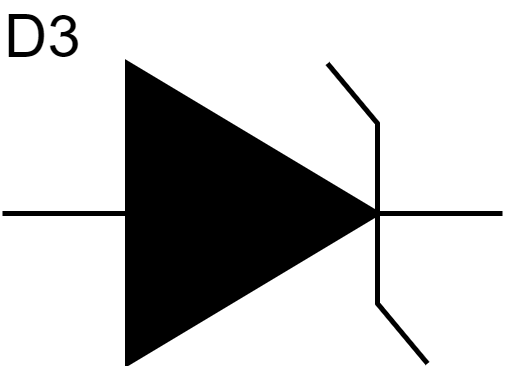
\includegraphics[height=1in]{electrical_schematics/zdiode_symbol.png}
            \caption[Zener Diode Symbol]{Schematic symbol for Zener diodes.}
        \end{figure}

        \paragraph*{Schottky Diode} are other special diodes that have a very low voltage drop across it, making it ideal for applications where flow restriction is necessary, but power loss needs to be considered.
        These are commonly used to control the flow of charge within a battery pack of multiple cells.
        As these cells discharge, they can have slightly different voltages, meaning some energy loss will occur as one battery tried to equalize voltage with another in the pack.
        Schottky diodes ensure the charges flow only from the batteries to the draw outside the pack, without wasting much energy.

        \begin{figure}[h!]
            \labfig{schottky_diode_symbol}
            \includegraphics[height=1in]{electrical_schematics/schdiode_symbol.png}
            \caption[Schottky Diode Symbol]{Schematic symbol for Schottky diodes.}
        \end{figure}

        \subsubsection*{Crystal Oscillators}
        Oscillators resonate at a certain frequency depending on the type of crystal used and the coupling capacitors matched to it.
        These driving most modern computational circuits as they generate a very clean DC square wave. 
        Some components use the rising or falling edge of this wave to trigger register shifts, calculations, anything else needed to perform its duty.
        Therefore, for any circuit that requires a high frequency, high reliability clock signal, most often, crystal oscillators will be present

        \begin{figure}[h!]
            \labfig{oscillator_symbol}
            \includegraphics[height=1in]{electrical_schematics/oscillator_symbol.png}
            \caption[Oscillator Symbol]{Schematic symbol for crystal oscillators.}
        \end{figure}

        \subsubsection*{Switches}
        Switches are mechanical contacts that physically direct the flow of electricity.
        They can have multiple independent circuits called "poles" that can allow current to flow from a common connector to an output connector called a "throw".
        They are named according to their architecture, e.g. Single Pole Double Throw (SPDT) switches have one circuit with two outputs that are connected to the common pin, depending on the switch position.
        Double Pole Triple Throw (DP3T) switches have two circuits that connect three output pins to a common input pin, depending on the switch position.
        Each circuit is mechanically linked so the same output connector in both circuits will be connected to the common.
        One downside to the mechanical switch is that they can be welded together if a maximum current is exceeded or, they can wear out over thousands of cycles.

        % \begin{marginfigure}[-3in]
        %     \labfig{switch_real}
        %     \includegraphics[]{electrical_schematics/switch.jpg}
        %     \caption{A common SPDT switch.
        %     Retrieved from \href{https://www.gardnerbender.com/en/p/GSW-12/SPDT-Toggle-Switch}{Gardner Bender}}
        % \end{marginfigure}

        \begin{figure}[h!]
            \labfig{switch_symbol}
            \includegraphics[height=1.5in]{electrical_schematics/switch_symbols.png}
            \caption[Switch Symbols]{Schematic symbols for different switch types.
            \emph{From left to right:} SPST, SPDT, DPDT.}
        \end{figure}

        \paragraph*{Buttons} are typically Single Pole Single Throw (SPST) switches that are spring loaded to remain normally open until pressed.
        When the button is pressed, a conducting plate makes contact with the common and output pins, completing the circuit through the button.
        These are commonly used as human input into circuits for calculations, state machines, typing lecture notes, etc.

        \begin{marginfigure}[-2in]
            \labfig{button_real}
            \includegraphics[]{electrical_schematics/button.jpg}
            \caption{A common push button found in most Arduino kits.
            Retrieved from \href{https://www.ebay.co.uk/itm/10-x-6x6x5mm-Momentary-Mini-Push-Button-Tactile-Switch-PCB-Mounted-SPST-/251779595483}{eBay}}
        \end{marginfigure}

        \begin{figure}[h!]
            \labfig{button_symbol}
            \includegraphics[height=0.75in]{electrical_schematics/button_symbol.png}
            \caption[Switch Symbols]{Schematic symbols for a normally open push button.}
        \end{figure}

        \paragraph*{Relays} are electromechanical switches that rely on an electromagnetic to move the electrical contact, rather than physical force.
        These are used for computers to manipulate large currents or direct electrical flow automatically, without human intervention.
        These relays follow the same nomenclature as normal switches and can be found in any number of configurations of poles and throws.

        \begin{figure}[h!]
            \labfig{relay_symbol}
            \includegraphics[height=1.5in]{electrical_schematics/relay_symbol.png}
            \caption[Switch Symbols]{Schematic symbols for an electromechanical relay.}
        \end{figure}

        \subsubsection*{Transistors}
        Transistors are electrical solid-state switches that use electrochemical properties to control the flow of electricity through them.
        These are typically able to withstand millions, if not billions, of switching cycles before failing and have driven the modern age we find ourselves in today.
        Everything in modern computing from the simple logic gate to the highest end computer and graphics processors use transistors to perform calculations or "think" about problems.
        Transistors have a gate that controls current flow from the source to the drain, depending on the voltage applied.

        \begin{marginfigure}[-1in]
            \labfig{transistor_real}
            \includegraphics[]{electrical_schematics/transistor.jpeg}
            \caption{A common transistor found in most Arduino kits.
            Retrieved from \href{https://www.walmart.com/ip/2N2222A-Plastic-Encapsulate-Power-Transistor-NPN-TO-92-25PCS/283496991}{Walmart}}
        \end{marginfigure}

        \begin{figure}[h!]
            \labfig{transistor_symbol}
            \includegraphics[height=1.5in]{electrical_schematics/transistor_symbol.png}
            \caption[Switch Symbols]{Schematic symbol for a transistor.}
        \end{figure}

        \paragraph*{MOSFETs} or Metal-Oxide-Semiconductor Field-Effect-Transistors are some of the most common types of transistors.
        They are able to be configured (doped) with different silicon structures that give them different electrochemical properties.
        N-Channel MOSFETs require a positive voltage on the Gate to function, whereas P-Channel MOSFETs require a negative gate voltage.
        Because of this, N-Channel MOSFETs are typically used for low-side switching (connect circuit to ground) and P-Channels are used for high switching (connect circuit to the voltage source). 
        There are two main types: depletion, which requires a Gate-Source voltage (Vgs) to switch the gate OFF, equivalent to a normally-closed switch; and enhancement where a Vgs is required to switch the gate ON, acting like a normally-open switch.
        These transistors are very common in high power applications and signal amplification.

        \begin{figure}[h!]
            \labfig{transistor_symbol}
            \includegraphics[height=1.5in]{electrical_schematics/pmosfet_symbol.png}
            \includegraphics[height=1.5in]{electrical_schematics/nmosfet_synmbol.png}
            \caption[Switch Symbols]{Schematic symbols for MOSFETs.
            On the left is a P-Channel MOSFET, on the right is an N-Channel MOSFET.}
        \end{figure}

        \todo{insert example from Thetis/EVE circuits - cherry pick some nice ones that use mostly discreet components}

    \subsection{Integrated Circuits}
    Integrated Circuits (ICs) comprise the backbone of modern electrical design.
    They combine any combination of discreet components, logic gates, processors, storage, etc. into a single package that can be easily placed into a circuit.
    For schematic symbols, the representation varies wildly, but generally hold to a few core design features:
        \paragraph*{Outlines} - represents the chip's presence on the schematic. 
        It encompasses all of the information about the IC and usually is large enough to fit descriptive text and allows the pins to be arranged in a cohesive manner.

        \paragraph*{Pins} - schematic representations of the chip's physical contacts with the circuit. 
        Each is uniquely coupled to the physical pin or pad on the real-world design, but does not have to be sequentially ordered in the schematic.
        Each pin should have a label for its purpose on the IC next to it, within the outline, as well as a label to identify its physical number on the IC.

        \paragraph*{Name} - this is the unique identifier of the IC on the schematic

        \paragraph*{Values} - this is typically the IC's part number for ordering information and implementation

    It is important to note that some IC symbols will opt to include other handy information in the outline so it is more easily accessible without having to refer back to the datasheet constantly.

    \todo{insert image of an IC symbol with leaders pointed to different parts}

    \todo{Inlcude image of IC circuits e.g. voltage regulator}
% ===========================================
% Data Processing
% Written by: Wensen Liu
%
% Date: 07/20/2022
% Last Revision: 07/20/2022
% ============================================

\setchapterstyle{kao}
\chapter{Software Basics and Architecture}
\setchapterpreamble[u]{\margintoc}
\labch{software_basics_and_arch}
% \addcontentsline{toc}{chapter}{Data Processing} % Add the preface to the table of contents as a chapter

While the world of physical hardware can be harnassed to develop systems that accomplish tasks, oftentimes these implementations become prohibitively complex as the scale of
implementation grows larger. For example, a modern computer processor contains billions of transistors and it would be impossible to set and reset each one of these transistors
by hand. Thankfully, as you probably already know, modern programming consists of several layers of abstraction above the transistor level, which allow us to develop meaningful
software solutions while leveraging the expansive amount of hardware that we have access to.

This chapter will focus on introducing you to the fundamentals of hardware-based software development. You may find that several if not all of these topics are also covered in
introductory programming courses. However, since we do not presume that everyone who has taken this class has had background programming experience, we will cover all the topics
necessary for this course from the ground up.

\section{Arduino Basics} \labsec{arduino_basics}
Lorem Ipsum Dolores

\section{Primitive Programming Datatypes} \labsec{primitive_programming_datatypes}
The baseline for every programming language is an understanding of datatypes.
Datatypes are how we can classify the characteristics of the blocks of information that our program will process.
These blocks of information can be collected data from the environment, information that the program stores internally, function inputs/outputs, etc.
Additional information on arduino datatypes (and in general, most arduino syntax) can be found on
\href{https://www.tutorialspoint.com/arduino/arduino_data_types.htm}{tutorialspoint} or the \href{https://www.arduino.cc/reference/en/}{Arduino Language Reference}
\marginnote{For the following sections, example code blocks will be given. As such, please note that the \enquote{$\backslash\backslash$} symbol is used to denote a \enquote{comment} and therefore
is not code that will execute and that the capitalization of keywords is deliberate (since Arduino C is case sensitive)}

    \subsection{void}
    The most basic of datatypes, the \textbf{void} keyword is used to represent \enquote{nothing}. For arduino programming, it is primarily used to denote that a function
    does not give us back any output. Do note, however, that the \textbf{void} datatype cannot be applied to variables.
    \marginnote{We will go more depth into functions in a later section, but for the purposes of this section you can think of functions as boxes that produce output from
    a given input. In the case of \textbf{void} we have no output.}
    
    \paragraph*{Proper usage of Void} The following code block demonstrates the proper usage of the \textbf{void} datatype.
    \begin{lstlisting}[linewidth=1.5\textwidth, language=C++]
        void function_name (\\ input variables) {
            \\ function code
            \\ note how there is no return statement (we are outputting nothing)
        }\end{lstlisting}

    \paragraph*{Improper usage of void} The following code block demonstrates the improper usage of the \textbf{void} datatype.
    \begin{lstlisting}[linewidth=1.5\textwidth, language=C++]
        void variable_name = \\ some value;\end{lstlisting}
    
    \subsection{bool}
    Boolean datatypes are used to store logic values, in this case the logic values of \textbf{True} or \textbf{False}. The \textbf{bool} keyword is used in both function and
    variable declarations to classify the function output or variable type as boolean logic.

    \paragraph*{Boolean usage} The following code block demonstrates how the \textbf{bool} keyword is used in a function declaration and a variable declaration
    \begin{lstlisting}[linewidth=1.5\textwidth, language=C++]
        bool function_name (\\ input variables) {
            bool variable_name = True;
            return variable_name;
        }\end{lstlisting}

    \subsection{Char}
    Character datatypes are special when programming in Arduino C. While they do represent what you would conventionally think as a character (for example, the letter \enquote{a}),
    they are defined based on their ascii value (\href{https://en.cppreference.com/w/cpp/language/ascii}{ASCII Reference}), which allow you to manipulate many more characters than
    what can be typed by a keyboard.

    The \textbf{char} keyword is used in variable and function declarations to classify the result as a character, and there are two ways to syntaxically represent a character.
    \paragraph*{Method 1: Using Single Quotes} The first form of syntax makes more sense visually, and involves wrapping a typed character within two single quotes
    \begin{lstlisting}[linewidth=1.5\textwidth, language=C++]
        char variable_name = 'a';\end{lstlisting}
    Do note, however, that this method restricts you to the characters that can be typed using a conventional keyboard. In addition, when declaring a character in this form, you
    cannot wrap multiple characters inside the quotes.
    \begin{lstlisting}[linewidth=1.5\textwidth, language=C++]
        char variable_name = 'abc'; \\ this is improper declaration \end{lstlisting}
    \paragraph*{Method 2: Using ASCII Values} As mentioned previously, characters are encoded via ASCII values when used in a programming context. As such, we can define a
    character using its corresponding ASCII value.
    \begin{lstlisting}[linewidth=1.5\textwidth, language=C++]
        char variable_name = 97; \\ ASCII value 97 corresponds to character 'a'\end{lstlisting}
    Since one character is equivalent to one byte of data, the maximum decimal value that can be used in a character declaration is 255.

    \begin{kaobox}[frametitle=Aside: Some quirks with characters]
        For all intents and purposes, characters are 8-bit binary numbers (0-255 in decimal). They become \enquote{characters} based on how they are interpreted when output to
        a display. Because of this dual interpretation, you can manipulate characters as if they were numbers. For example
        \begin{equation*}
            'a' + 1 = 'b'
        \end{equation*}
        However, if you were to use \enquote{1} (the character representation of 1) as the input you would get
        \begin{equation*}
            'a' + '1' = 97 + 49 = 156
        \end{equation*} 
        Which, for those that are curious, 156 represents the ASCII character \oe. In addition, there are special characters that can be typed using the single quotes 
        method that do not strictly follow the \enquote{only one character} rule. In particular, the $'\backslash n'$ (newline) and $'\backslash t'$ (tab) characters are often used.
    \end{kaobox}

    \subsection{unsigned char and byte}
    The unsigned character and byte datatypes are both datatypes that are used to represent a byte of data (8 bits, 0-255 in decimal). While they share the same range of values
    as the char datatype, they should not be used interchangeably with the char datatype. The \textbf{unsigned char} and \textbf{byte} keywords are used to define function output
    and variable values.
    \marginnote{Generally speaking, it is conventional to use the \textbf{byte} keyword over the \textbf{unsigned char} keyword for both brevity and code readability}
    \paragraph*{unsigned char and byte usage} the following block of code demonstrates how to use the \textbf{unsigned char} and \textbf{byte} keywords
    \begin{lstlisting}[linewidth=1.5\textwidth, language=C++]
        byte function_name (\\ input variables) {
            byte variable_name_1 = 0;
            unsigned char variable_name_2 = 128;
            return variable_name_1;
        }\end{lstlisting}

    \subsection{int and short}
    Both the \textbf{int} datatype and the \textbf{short} datatype are used to store 16-bit (2 byte) signed integers. This makes their effective range -32,768 to 32,767. By convention, the \textbf{int} datatype
    is the more commonly used one in variable and output declaration.
    \marginnote{One of the things that you will have to look out for when using numeric datatypes is \textbf{overflow}; ie. when the number passed into a data field is larger than the range of that datatype.
    Overflow will \textbf{not} stop the code from compiling, but the code's behavior will arbitrarily differ from what you expect.}
    \paragraph*{int and short usage} the following block of code demonstrates how to use the \textbf{int} and \textbf{short} keywords
    \begin{lstlisting}[linewidth=1.5\textwidth, language=C++]
        int function_name (\\ input variables) {
            int variable_name_1 = -20000;
            short variable_name_2 = 12763;
            return variable_name_1;
        }\end{lstlisting}
    
    \subsection{unsigned int and word}
    Similar to the case with \textbf{char} and \textbf{unsigned char}, there are also unsigned variants of the \textbf{int} and \textbf{short} datatypes respectively known as \textbf{unsigned int} and
    \textbf{word}. These datatypes are both 16-bit(2 byte) integers; however, they span only the \textbf{positive} range of 16-bit integers (0 to 65,535).
    \marginnote{The \textbf{unsigned int} datatype has \textbf{known} overflow behavior unlike \textbf{int}. When the value of an unsigned integer goes below zero, it wraps around to the max of the
    range (so -1 = 65535, -2 = 65534) and when it exceeds 65535, it wraps back to zero (so 65536 = 0, 65537 = 1)}
    \paragraph*{unsigned int and word usage} the following block of code demonstrates how to use the \textbf{unsigned int} and \textbf{word} keywords
    \begin{lstlisting}[linewidth=1.5\textwidth, language=C++]
        unsigned int function_name (\\ input variables) {
            unsigned int variable_name_1 = 1203;
            word variable_name_2 = 55000;
            return variable_name_1;
        }\end{lstlisting}
    
    \subsection{long and unsigned long}
    We had previously covered that a \textbf{short} is a 16-bit integer. Therefore, appropriately, a \textbf{long} is a 32-bit signed integer value encompassing the range -2,147,483,648 to 2,147,483,647. As
    per convention, the \textbf{unsigned long} store a 32-bit unsigned integer value with range 0 to 4,294,967,295.
    \paragraph*{long and unsigned long usage} the following block of code demonstrates how to use the \textbf{long} and \textbf{unsigned long} keywords
    \begin{lstlisting}[linewidth=1.5\textwidth, language=C++]
        long function_name (\\ input variables) {
            long variable_name_1 = -2000000;
            unsigned long variable_name_2 = 1000000;
            return variable_name_1;
        }\end{lstlisting}
    
    \subsection{float and double}
    There are also datatypes that are used to store decimal values vs. pure integer, these are the \textbf{float} and \textbf{double} datatypes. For the boards that you will be using, the \textbf{float} and
    the \textbf{double} datatypes are functionally the same. They both cover the range -3.4028235E+38 to 3.4028235E+38, and are both stored in memory as 32-bit values. 
    \paragraph*{float and double usage} the following block of code demonstrates how to use the \textbf{float} and \textbf{double} keywords
    \begin{lstlisting}[linewidth=1.5\textwidth, language=C++]
        float function_name (\\ input variables) {
            float variable_name_1 = -300.21;
            double variable_name_2 = 600.123;
            return variable_name_1;
        }\end{lstlisting}
    \paragraph*{Floating point error} One of the issues that you may run into when dealing with floats and doubles is the floating point (roundoff) error. Due to how floating point numbers are represented
    (for more info on that, you can read up on the \href{https://en.wikipedia.org/wiki/IEEE_754}{IEEE-754 Standard}), and due to the fact that floating point numbers are stored in a finite number of bits (32),
    floating point numbers are \textbf{not absolutely accurate} and will differ from the true value of a datapoint by a small amount. For the majority of applications, this slight difference between 
    actual values and real values is trivial and non-impactful to the application. However, for applications that store small magnitude numbers as data, or rely on high-precision calculations, floating
    point error is something to watch out for.
    
    \subsection{Arrays}
    Arrays are one of the most fundamental structures to understand when working with any programming language. In Arduino C, they are treated as a block of memory that is broken up into chunks, where each
    chunk stores a single value of a datatype. Arrays in Arduino follow an explicit set of rules that govern how they are defined and used, which we will cover below.
    \paragraph*{Rule 1: Arrays can only hold 1 data type} Unlike some other languages, an array in Arduino (and in C in general) must be defined to store a single datatype. You cannot have an array that has
    both int and float datatypes for example. For the reasoning behind this rule, you can take a look at the following aside.
    \paragraph*{Rule 2: Arrays must have a predefined number of values} When you initialize an array, you must tell the program how many values are going to be stored in the array. After this declaration, you 
    cannot modify the size of that array. The reasoning behind this rule is also covered in the following aside.
    \begin{kaobox}[frametitle=Aside: The weird world of memory allocation]
        C (and its variants) are programming languages that deal directly with memory. While this makes them faster than languages that do not directly modify memory, it also restricts how flexible variables
        and memory structures can be when using them. When reading or writing to memory, the amount of memory you use and how that memory will be divided up must be explicitly defined. If the variable asks 
        for 32 bits of memory, it will get 32 bits of memory, no more, no less. In a similar sense, arrays also must explicitly define how much memory they will use. An array that wants to store 10 ints 
        (16-bit) will be allocated $10 * 16 = 160$ bits of memory divided into 10x 16-bit chunks. If you tried to store a long (32-bit) into one of those chunks, it will not fit and the program will error. Now,
        while it is possible to allocate a raw chunk of memory to be manually partitioned and used, how to do that is beyond the scope of this class. Those interested can read up on \textbf{memory allocation
        in C}
    \end{kaobox}
% ===========================================
% Data Processing
% Written by: Braidan Duffy
%
% Date: 06/22/2022
% Last Revision: 06/22/2022
% ============================================

\setchapterstyle{kao}
\chapter{Data Processing}
\setchapterpreamble[u]{\margintoc}
\labch{data_processing}
% \addcontentsline{toc}{chapter}{Data Processing} % Add the preface to the table of contents as a chapter

Data collected from sensors can sometimes be useful on their own, but often times, it is necessary to process it to gain a better understanding of what is occurring.
To that end, this chapter will be about how to process raw data into something more usable and some techniques that you can employ for your projects in the future.

    \section{Digital Filtering} \labsec{digital_filtering}
    One of the most fundamental data processing techniques is that of the digital filter.
    The idea behind these filters is to take in data samples and apply mathematical formulations on them to dampen undesirable signals within.
        
        \subsection{Background} This section assumes that you do not have a lot of background knowledge on basic statistics and terminology.
        It is important to understand here that mean and expected value are not the same thing.
        In many college lab courses, measurements are taken multiple times and averaged together to find the mean value (often denoted as $\mu$).
        This is assumed to be the absolute correct value with zero uncertainty.
        However, this is never the case in the real world as all measurements have uncertainty in some fashion.
        When the average measurement value is taken \textit{with} uncertainties factored in, this becomes the expected value ($E$) and used to guess what the real (correct) value of the measured variable is.

        So, how can quantify the uncertainties within the expected value? First, we need to know what the measurement variance is.
        This value is a description of how far the measured data is from the mean and is defined in Equation \ref{eq:variance}. \sidenote{For large datasets, variance is normalized by $\frac{1}{N-1}$}

        \marginnote{The standard deviation of the dataset $\sigma$ decribes the probabalistic distance a measurement can have from the mean and is defined by:
        \begin{equation*}
            \sigma = \sqrt{\sigma^2}
        \end{equation*}
        }
        
        \begin{gather} \labeq{variance}
            \sigma^2 = \frac{1}{N} \sum_{n=1}^{N} (x_n - \mu)^2 \\ 
            \begin{aligned}
                \text{where } &\sigma^2 \text{ is the variance} \\
                &N \text{ is the total number of samples} \\
                &x_n \text{ is the n-th sample} \\
                &\mu \text{ is the running average}
            \end{aligned} \notag
        \end{gather}

        \begin{kaobox}[frametitle=Aside: Normal Distribution]
            Normal distribution of data is the archetypical bell curve.
            It is also referred to Gaussian distribution and is defined by:
            \begin{equation*}
                f(x, \mu, \sigma^2) = \frac{1}{2\pi\sigma^2} \exp{\frac{-(x-\mu)^2}{2\sigma^2}}
            \end{equation*}
            This function creates a Gaussian curve which is the Probability Density Function (PDF) for a normal distribution.
            Normally, measurements errors are Gaussian-distributed and the Kalman filter assumes this is always the case.
            Different error distributions will drastically increase the uncertainties within the filter and may negate it entirely.
        \end{kaobox}
        
        \begin{marginfigure}[-2in]
            \includegraphics[]{data_processing/gaussian_distribution.png}
            \caption[Aside: Gaussian Distribution]{A graph of a Gaussian distribution with the 1st standard deviations shown.
            Retrieved from \href{https://accadandkoka.com/blog/how-normal-is-the-normal-distribution/}{The Akkad and Koda Report}}
            \labfig{aside_gaussian_dist}
        \end{marginfigure}

        Estimates are the algorithm's guessed value at the unknown system state.
        Here, accuracy quantifies how close the estimate is to the true value whereas precision quantifies the variability of the estimates with respect to uncertainty.
        High precision estimates have a low variance (uncertainty) in measurements.
        Low accuracy estimates display a bias that are systemic errors in measurement.
        Variance is determined by random measurement error and can be reduced by averaging or smoothing the measurements.

        \begin{figure*}[h!]
            \includegraphics[]{data_processing/AccuracyAndPrecision.png}
            \caption[Accuracy and Precision]{Different plots demonstrating the difference between accuracy and precision.
            Retrieved from \href{https://www.kalmanfilter.net/img/BB1/AccuracyAndPrecision.png}{KalmanFilter.net}}
            \labfig{accuracy_precision}
        \end{figure*}

        \subsection{The $\alpha$ Filter} 
        At any sample, $N$, a value $\hat{x}_{N,N}$ can be estimated using:
        
        \begin{gather*} \labeq{sample_estimate}
            \hat{x}_{n,n} = \frac{1}{N} \sum_{n=1}^{N} (z_n) \\
            \begin{aligned}
                \text{where } &\hat{x}_{n,n} \text{is the estimate of the true value at sample $n$} \\
                &N \text{ is the total number of samples taken} \\
                &n \text{ is the current sample number} \\
                &z \text{ is the current measurement} \\
            \end{aligned} \notag
        \end{gather*}

        Since the estimate accuracy will improve with the number of measurements, we need to remember all the historical measurements.
        However, storing, accessing, and operating on discrete measurements exponentially increases in difficulty and computational power as more measurements are taken.
        Therefore, we can store the previous measurements in a state variable and add a small adjustment that is proportional to the newest measurement.
        This preserves the accuracy of storing many discrete data points and the computing and storage resources required to operate on data added to the set.

        This algorithm is called the \textit{State Update Equation} and is one of the five Kalman equations. 
        It is defined by:

        \begin{gather} \labeq{state_update_eq}
            \hat{x}_{n,n} = \hat{x}_{n,n-1} + \alpha_n(z_n - \hat{x}_{n,n-1}) \\
            \begin{aligned}
                \text{where } &\hat{x}_{n,n} \text{is the estimate of the true value at sample $n$} \\
                &\hat{x}_{n,n-1} \text{ is the estimate of the previous true value} \\
                &n \text{ is the current sample number} \\
                &\alpha_n \text{ is a correction gain} \\
                &z \text{ is the current measurement} \\
            \end{aligned} \notag
        \end{gather}

        \marginnote[-1.5in]{The correction gain, $\alpha_n$ is unique to every example and can change with every sample.
        It is also called the Kalman gain, denoted by $K_n$}

        \marginnote[-0.75in]{The term $(z_n - \hat{x}_{n,n-1})$ is the measurement residual or "innovation"; this contains the new information.}

        This algorithm uses zero-indexing, so the initial or starting guess will be $n=0$.
        This value can be determined by reasoning or physical constraints of the system.
        The filter will always require an initial guess to kickstart the algorithm.
        A flow chart describing the algorithm's process is below.
        
        \pagelayout{wide} % No margins

        \begin{example} \label{ex:alpha_filter}
        Let's say that we are programming a scale to estimate the weight of an ROV placed atop it.
        For the sake of example, we know that the ROV weighs exactly 10 kilograms and we want to quantify the uncertainty of our scale.
        \paragraph{Iteration 0}
        \begin{equation*}
            \begin{aligned} 
                0:& \text{ We can guess that the initial weight of the ROV is 10-kg: } \hat{x}_{0,0} = 10 \text{ kg} \\
                3:& \text{ Since the weight should not change, our prediction for the next measurement is: } \hat{x}_{1,0} = \hat{x}_{0,0} = 10 \text{ kg} \\
            \end{aligned}
        \end{equation*}
        
        \paragraph{Iteration 1}
        \begin{equation*}
            \begin{aligned} 
                1:& \text{ We make a measurement on the scale: } z_1 = 10.3 \text{ kg} \\
                2\text{a}:& \text{ We calculate the correction gain: } \alpha_1 = \frac{1}{N} = \frac{1}{1} = 1 \\
                2\text{b}:& \text{ We can then estimate the current state: } \hat{x}_{1,1} = \hat{x}_{1,0} + \alpha_1(z_1 - \hat{x}_{1,0}) = 10 + 1(10.3 - 10) = 10.3 \text{ kg} \\
                3:& \text{ Since the weight should not change: } \hat{x}_{2,1} = \hat{x}_{1,1} = 10.3 \text{ kg} \\
            \end{aligned}
        \end{equation*}

        \paragraph{Iteration 2}
        \begin{equation*}
            \begin{aligned} 
                1:& \text{ We make a measurement on the scale: } z_2 = 9.9 \text{ kg} \\
                2\text{a}:& \text{ We calculate the correction gain: } \alpha_2 = \frac{1}{N} = \frac{1}{2} = 0.5 \\
                2\text{b}:& \text{ We can then estimate the current state: } \hat{x}_{2,2} = \hat{x}_{2,1} + \alpha_2(z_2 - \hat{x}_{2,1}) = 10.3 + 0.5(9.9 - 10.3) = 10.1 \text{ kg} \\
                3:& \text{ Since the weight should not change: } \hat{x}_{3,2} = \hat{x}_{2,2} = 10.1 \text{ kg} \\
            \end{aligned}
        \end{equation*}

        The calculations and results for this example are summarized in the table and figure below:

        \begin{center}
            \begin{tabular}{c | c | c | c | c}
            \toprule
            & \multicolumn{3}{|c|}{Current Estimates} & Predictions \\
            \midrule
            n & $z_n$ & $\alpha_n$ & $\hat{x}_{n,n}$ & $\hat{x}_{n+1,n}$ \\
            \midrule

            0  & ---- &      ----      & 10.0 & 10.0 \\[4pt]
            1  & 10.3 &       1        & 10.3 & 10.3 \\[4pt]
            2  &  9.9 & $\frac{1}{2 }$ & 10.1 & 10.1 \\[4pt]
            3  &  9.8 & $\frac{1}{3 }$ & 10.0 & 10.0 \\[4pt]
            4  & 10.3 & $\frac{1}{4 }$ & 10.1 & 10.1 \\[4pt]
            5  & 10.4 & $\frac{1}{5 }$ & 10.1 & 10.1 \\[4pt]
            6  & 10.1 & $\frac{1}{6 }$ & 10.1 & 10.1 \\[4pt]
            7  & 10.3 & $\frac{1}{7 }$ & 10.2 & 10.2 \\[4pt]
            8  & 10.0 & $\frac{1}{8 }$ & 10.1 & 10.1 \\[4pt]
            9  &  9.8 & $\frac{1}{9 }$ & 10.1 & 10.1 \\[4pt]
            10 &  9.5 & $\frac{1}{10}$ & 10.0 & ---- \\[4pt]

            \bottomrule
            \end{tabular}
        \end{center}

        \begin{center}
            \includegraphics[height=3.5in]{examples/alpha_filter_results.png}
        \end{center}

        The $\alpha$-filter considerably smoothed out the noisy measurement data and will eventually converge on an estimate close to the true value (within 10\%).

        \end{example}

        \pagelayout{margin} % Replace margins

        \subsection{The $\alpha$ and $\beta$ Filter}
        As demonstrated in Example \ref{ex:alpha_filter}, the $\alpha$ filter makes a major assumption that the state does not change between samples.
        In reality, this is rarely the case as we typically want to measure a body's movement, or track a variable over time, or measure something that has dependency on another variable.
        
        For example, if we wished to track a boat moving in a one-dimensional world at a constant velocity (no acceleration), we need to modify our model a bit.
        For nomenclature, $x_n$ will represent the displacement of the vessel from a known starting point.
        Since the vessel is moving with a constant velocity, we can model its time rate of change of position as:
        
        \begin{equation*}
            \dot{x} = v = \frac{dx}{dt}
        \end{equation*}

        If we sample the vessel's displacement at intervals of $\Delta t$ time, then we can define a dynamic model of the vessels movement as:

        \begin{subequations}
            \labeq{see_dynamic_model}
            \begin{align}
                x_{n+1} &= x_n + \Delta t \dot{x}_n \labeq{see_disp}\\
                \dot{x}_{n+1} &= \dot{x}_n \labeq{see_velocity}
            \end{align}
        \end{subequations}

        This is called the \textit{State Extrapolation Equation} \sidenote{or the \textit{State Transistion Equation} or the \textit{State Prediction Equation}} and is another one of the five Kalman equations.
        If we assume the sample interval is $\Delta t = 5 \text{ seconds}$ at sample $n-1$ and the displacement and velocity of the vessel is estimated as 300-m and 10-m/s, respectively, then using Equations \ref{eq:see_disp} and \ref{eq:see_velocity}, we can predict where the vessel will be and its velocity at sample $n$.
        
        \begin{equation*}
            \begin{gathered}
                \hat{x}_{n,n-1} = \hat{x}_{n-1,n-1} + \Delta t \hat{\dot{x}}_{n-1,n-1} = 300 + 5(10) = 350 \text{ m} \\
                \hat{\dot{x}}_{n,n-1} = \hat{x}_{n-1,n-1} = 10 \text{ m/s}
            \end{gathered}
        \end{equation*}

        However, at sample $n$, the vessel records a displacement of 320-m, not the expected 350-m; there are two possible reasons:

        \begin{enumerate}
            \item the vessel displacement measurements are not precise or accurate
            \item the vessel velocity changed unexpectedly \sidenote{The new velocity would have to be:
                                                                        \begin{equation*}
                                                                            \frac{320-300}{5} = 4 \text{ m/s}
                                                                        \end{equation*}}
        \end{enumerate}

        We know from the previous section that we can account for the measurement error using an $\alpha$ filter, so lets re-write Equation \ref{eq:see_velocity} to account for error in the velocity:

        \begin{equation}
            \labeq{see_velocity_b}
            \hat{\dot{x}}_{n,n} = \hat{\dot{x}}_{n,n-1} + \beta(\frac{z_n - \hat{x}_{n,n-1}}{\Delta t})
        \end{equation}

        \pagelayout{wide} % Remove margins

        \begin{example} \label{ex:alpha_beta_filter}
        Consider a boat moving in one dimension. 
        We are going to assume the following:
        \begin{itemize}
            \item $\alpha = 0.2$ (Positional gain)
            \item $\beta = 0.1$ (Velocity gain)
            \item $\Delta t = 5$ seconds
        \end{itemize}

        \paragraph{Iteration 0}
        \begin{equation*}
            \begin{aligned} 
                0:& \text{ Initial conditions: } \hat{x}_{0,0} = 300 \text{ m, } \hat{\dot{x}}_{0,0} = 4 \text{ m/s} \\
                3:& \text{ Predict the next position: } \hat{x}_{1,0} = \hat{x}_{0,0} + \Delta t \hat{\dot{x}}_{0,0} = 300 + 5(4) = \textbf{320 m} \\
                 :& \text{ Predict the next velocity: } \hat{\dot{x}}_{1,0} = \hat{\dot{x}}_{0,0} = \textbf{4 m/s}
            \end{aligned}
        \end{equation*}
        
        \paragraph{Iteration 1}
        \begin{equation*}
            \begin{aligned} 
                1:& \text{ The vessel makes a positional measurement: } z_1 = \textbf{310 m} \\
                2:& \text{ We estimate the current position: } \hat{x}_{1,1} = \hat{x}_{1,0} + \alpha(z_1 - \hat{x}_{1,0}) = 320 + 0.2(310 - 320) = \textbf{318 m} \\
                 :& \text{ We estimate the current velocity: } \hat{\dot{x}}_{1,1} = \hat{\dot{x}}_{1,0} + \beta(\frac{z_1 - \hat{x}_{1,0}}{\Delta t}) = 4 + 0.1(\frac{310 - 320}{5}) = \textbf{3.8 m/s} \\
                3:& \text{ Predict the next position: } \hat{x}_{2,1} = \hat{x}_{1,1} + \Delta t \hat{\dot{x}}_{1,1} = 318 + 5(3.8) = \textbf{337 m} \\
                 :& \text{ Predict the next velocity: } \hat{\dot{x}}_{2,1} = \hat{\dot{x}}_{1,1} = \textbf{3.8 m/s}
            \end{aligned}
        \end{equation*}

        \paragraph{Iteration 2}
        \begin{equation*}
            \begin{aligned} 
                1:& \text{ The vessel makes a positional measurement: } z_2 = \textbf{317 m} \\
                2:& \text{ We estimate the current position: } \hat{x}_{2,2} = \hat{x}_{2,1} + \alpha(z_2 - \hat{x}_{2,1}) = 337 + 0.2(317 - 337) = \textbf{333 m} \\
                 :& \text{ We estimate the current velocity: } \hat{\dot{x}}_{2,2} = \hat{\dot{x}}_{2,1} + \beta(\frac{z_2 - \hat{x}_{2,1}}{\Delta t}) = 3.8 + 0.1(\frac{337 - 317}{5}) = \textbf{3.4 m/s} \\
                3:& \text{ Predict the next position: } \hat{x}_{3,2} = \hat{x}_{2,2} + \Delta t \hat{\dot{x}}_{2,2} = 333 + 5(3.4) = \textbf{350 m} \\
                 :& \text{ Predict the next velocity: } \hat{\dot{x}}_{3,2} = \hat{\dot{x}}_{2,2} = \textbf{3.4 m/s}
            \end{aligned}
        \end{equation*}

        The data for this example is summarized in the table and figure below:

        \begin{center}
            \begin{tabular}{c | c | c | c | c | c}
            \toprule
            & \multicolumn{3}{|c|}{Current Estimates} & \multicolumn{2}{c}{Predictions} \\
            \midrule
            n & $z_n$ & $\hat{x}_{n,n}$ & $ \hat{\dot{x}}_{n,n} $ & $ \hat{x}_{n+1,n}$ & $ \hat{\dot{x}}_{n+1,n} $ \\
            \midrule

            0  &  ---  & 300.0 & 4.00 & 320.0 & 4.00 \\
            1  & 322.0 & 320.4 & 4.04 & 340.6 & 4.04 \\
            2  & 341.0 & 340.7 & 4.05 & 360.9 & 4.05 \\
            3  & 358.0 & 360.3 & 3.99 & 380.3 & 3.99 \\
            4  & 374.0 & 379.0 & 3.86 & 398.3 & 3.86 \\
            5  & 399.0 & 398.5 & 3.88 & 417.9 & 3.88 \\
            6  & 420.0 & 418.3 & 3.92 & 437.9 & 3.92 \\
            7  & 436.0 & 437.5 & 3.88 & 456.9 & 3.88 \\
            8  & 458.0 & 457.1 & 3.90 & 476.7 & 3.90 \\
            9  & 483.0 & 477.9 & 4.03 & 476.7 & 4.03 \\
            10 & 501.0 & 498.7 & 4.09 & 498.1 & 4.03 \\

            \bottomrule
            \end{tabular}
        \end{center}

        \begin{center}
            \includegraphics[height=3in]{examples/ex_6_4_alpha_beta_filter_results.png}
        \end{center}

        From the figure, we can see that the filter provides a good "smoothing" effort for the noisy measurement data.
        High values for $\alpha$ and $\beta$ will result in less "smoothing" in certain cases.
        The current state estimate may be very close to the measurement values with a higher error in predicted values

        The value of $\beta$ depends on the precision of the vessel's navigation system.
        If the positional precision is $\sigma = 0.1 \text{ m}$, then it is very likely the vessel speed changed.
        Therefore, $\beta$ would be very high to adjust the estimated velocity.
        Conversely, if the positional precision is $\sigma = 10 \text{ m}$, then it is likely the vessel's position measurements are wrong and $\beta$ can be smaller.

        $\alpha$ and $\beta$ depend on the measurement precision.
        Very precise measurements would prefer a high $\alpha$ and $\beta$ gains that will cause the filter to converge quickly and can adapt to velocity changes.
        Lower precision measurements would prefer lower $\alpha$ and $\beta$ gains that allow any uncertainties to be smoothed out; this will cause the filter to react slowly to velocity changes or external perturbations, though.
        
        \end{example}

        \pagelayout{margin} % Restore margins

        \paragraph{The Importance of Accurate Modelling} Lets expand upon Example \ref{ex:alpha_beta_filter}.
        Here, we will consider the same vessel under the same assumptions and initial conditions, but we will have a flawed dynamic model.
        The vessel will begin transiting at a constant velocity of 5-m/s for 15 seconds, then accelerate at a constant 2-m/s/s for 15 seconds.
        The kinematic plots are displayed below in Figure \ref{fig:alpha_beta_acc} and the numerical results can be found in Table \ref{tab:alpha_beta_acc}.

        \begin{table}[h!]
            \labtab{alpha_beta_acc}
            \begin{tabular}{c | c | c | c | c | c}
            \toprule
            & \multicolumn{3}{|c|}{Current Estimates} & \multicolumn{2}{c}{Predictions} \\
            \midrule
            n & $z_n$ & $\hat{x}_{n,n}$ & $ \hat{\dot{x}}_{n,n} $ & $ \hat{x}_{n+1,n}$ & $ \hat{\dot{x}}_{n+1,n} $ \\
            \midrule

            0  & ----- & 30.0  & 5.00 & 55.0  & 5.00 \\
            1  & 60.0  & 56.0  & 5.10 & 81.5  & 5.10 \\
            2  & 77.0  & 80.6  & 5.01 & 105.7 & 5.01 \\
            3  & 107.0 & 105.9 & 5.03 & 131.1 & 5.03 \\
            4  & 154.0 & 135.7 & 5.50 & 163.2 & 5.50 \\
            5  & 252.0 & 181.0 & 7.30 & 217.5 & 7.30 \\
            6  & 407.0 & 255.4 & 11.1 & ----- & ---- \\

            \bottomrule
            \end{tabular}
            \caption[Alpha-Beta Filter with Lag]{Numerical results for the $\alpha-\beta$ filter not accounting for acceleration}
        \end{table}

        \begin{figure}[h!]
            \labfig{alpha_beta_acc}
            \includegraphics[height=3.5in]{examples/alpha_beta_filter_acc_results.png}
            \caption[Alpha-Beta Filter Results with Lag]{Graphical results for the $\alpha-\beta$ filter not accounting for acceleration}
        \end{figure}

        The difference between the real plot (black) and the estimated plot (blue) is called the lag error.
        The lag error causes the estimates to drastically diverge from the real values as they change with time.
        Increasing the $\beta$ gain may allow the estimates to converge faster to the real values, but there is a better way.

        \subsection{The $\alpha$ $\beta$ and $\gamma$ Filter}
        This next filter considers the change of the rate of the change variable. 
        In the case of moving targets, this means acceleration.
        This changes the State Extrapolation Equations to:

        \begin{subequations}
            \labeq{see_dynamic_model_2}
            \begin{align}
                \hat{x}_{n+1,n} &= \hat{x}_{n,n} + \Delta t \hat{\dot{x}}_{n,n} + \frac{1}{2} \hat{\ddot{x}}_{n,n} {\Delta t}^2 \labeq{see_disp_2}\\
                \hat{\dot{x}}_{n+1,n} &= \hat{\dot{x}}_{n,n} + \hat{\ddot{x}}_{n,n} \Delta t \labeq{see_velocity_2} \\
                \hat{\ddot{x}}_{n+1,n} &= \hat{\ddot{x}}_{n,n}
            \end{align}
        \end{subequations}

        Similarly, the State Update Equations become:

        \begin{subequations}
            \labeq{sue_abg}
            \begin{align}
                \hat{x}_{n,n} &= \hat{x}_{n,n-1} + \alpha (z_n - \hat{x}_{n,n-1}) \labeq{sue_abg_disp}\\
                \hat{\dot{x}}_{n,n} &= \hat{\dot{x}}_{n,n-1} + \beta (\frac{z_n - \hat{x}_{n,n-1}}{\Delta t}) \labeq{sue_abg_velocity} \\
                \hat{\ddot{x}}_{n,n} &= \hat{\ddot{x}}_{n,n-1} + \gamma (\frac{z_n - \hat{x}_{n,n-1}}{\frac{1}{2} \Delta t^2}) \labeq{sue_abg_accel}
            \end{align}
        \end{subequations}

        This type of filter eliminates the lag error by accounting for a constant acceleration.
        If we want to account for "jerk", or a change in acceleration, we need to implement a more advanced filter like the Kalman filter.

        \subsection{Kalman Filter} \labsec{kalman_filter}
        \subsubsection*{Introduction} 
        The Kalman Filter is a recursive algorithm introduced in the 1960's as a method to track, estimate, and predict the state of a system and corresponding uncertainties.
        This filter integrates a dynamic (linear) model of the system, control inputs, measurements, and biases/uncertainties into a single algorithm.
        This effectively fuses together system inputs and responses and extrapolates what the system is currently doing and expected to do.
        One key advantage of this algorithm is that it only requires the guess of the previous state to estimate the current state. 
        This massively decreases the memory and processing costs as the history of inputs, measurements, and uncertainties does not need to be remembered or analyzed.
        However, it does have some limitations when the sensor data is noisy or the control inputs cannot be linearly mapped to the system state.
        Random errors in the sensor data may cause the filter to behave unpredictably and non-linearity prevents proper fusion entirely.\sidenote{Though this can be managed with an Extended Kalman Filter}

        This section will discuss the Kalman filter in a higher-order method.
        Many resources around with Internet can discuss the in-depth mathematics governing this filter and you are free to browse them at your leisure. 
        For this guide, my primary concern is to get you acquainted with the Kalman filter and its broader practical applications.

        \subsubsection*{Kalman Filter in One Dimension}
        The uni-dimensional Kalman filter is a special, idealized case for the Kalman filter.
        It is more convenient as a teaching tool as it does not include the complex matrix and vector operations the general multi-dimensional Kalman filter requires.
        However, this only makes this type useful for tracking and estimating a single variable.

        Multiple uni-dimensional Kalman filters can be run in parallel or chained together to mimic a multi-dimensional filter, however, this will unnecessarily increase the computational resources required for the calculations and will reduce the quality of the filtering overall.

        \paragraph*{The Kalman Gain} In a Kalman filter, the $\alpha-\beta-\gamma$ parameters are calculated at every filter iteration.
        These parameters are combined together into the Kalman Gain, denoted as $K_n$, which is the third Kalman equation.
        The Kalman gain is bounded by: $0 <= Kn <= 1$.

        \begin{equation} \labeq{kalman_gain}
            \begin{aligned}
                K_n &= \frac{\text{Estimate Uncertainty}}{\text{Estimate Uncertainty + Measurement Uncertainty}} \\
                    &= \frac{p_{n,n-1}}{p_{n,n-1} + r_n}
            \end{aligned}
        \end{equation}

        If we refresh the State Update Equation (Eq. \ref{eq:state_update_eq}) with the Kalman gain, we get:

        \begin{equation} \labeq{kalman_state_update_eq}
            \begin{aligned}
                \hat{x}_{n,n} &= \hat{x}_{n,n-1} + K_n(z_n - \hat{x}_{n,n-1}) \\
                              &= (1-K_n)\hat{x}_{n,n-1} + K_n z_n \\
            \end{aligned}
        \end{equation}

        In the above equation, $K_n$ is the weight (importance) given to the measurement.
        Conversely, $(1-K_n)$ is the weight given to the estimate.

        \marginnote[-1.5in]{\textbf{Important note:} When measurement uncertainty is very large, and the estimate uncertainty is small, $K_n << 1$, hence big weight to the estimate and small weight to the measurement. When the opposite is true, $K_n -> 1$, meaning a large weight to the measurement and a small weight to the estimate. This is how the Kalman filter can regulate and smooth out noisy data by knowing the uncertainties.}

        \paragraph*{The Estimate Uncertainty Update Equation} the fourth Kalman equation is the \textit{Estimate Uncertainty Update}. \sidenote{Also referred to as the \textit{Covariance Update Equation}.}
        The estimate uncertainty should approach (converge) to 0 with each filter iteration as the filter improves its guessing accuracy.
        However, if the measurement uncertainty is large ($K_n << 1$), the estimate uncertainty will converge more slowly.
        The opposite is true if the measurement uncertainty is small.
        Basically, the more precise your measurements are, the faster the Kalman filter will converge on the best estimate.

        \begin{gather}
            p_{n,n} = (1-K_n)p_{n,n-1} \\
            \begin{aligned}
                \text{where } &p_{n,n} \text{ is the estimate uncertainty at the current state} \\
                              &K_n \text{ is the Kalman gain at the current state} \\
                              &p_{n,n-1} \text{ is the estimate uncertainty of the previous state}
            \end{aligned} \notag
        \end{gather}

        \paragraph*{The Estimate Uncertainty Extrapolation Equation} The fifth and final Kalman equation is how the filter predicts future uncertainties and is called the \textit{Estimate Uncertainty Extrapolation Equation}. \sidenote{Also referred to as the \textit{Covariance Extrapolation Equation}}
        Like with the State Extrapolation Equations, this is done with dynamic models and will be unique to every example.
        If we refer to the previous models from Equations \ref{eq:see_disp} and \ref{eq:see_velocity}, we can define the Estimate Uncertainty Extrapolation Equations as:

        \begin{subequations}
            \labeq{covariance_extrapolation}
            \begin{align}
                p_{n+1,n}^x &= p_{n,n}^x + \Delta t p_{n,n}^{\dot{x}} \\
                p_{n+1,n}^{\dot{x}} &= p_{n,n}^{\dot{x}}
            \end{align}
        \end{subequations}

        For more information on variance and its derivation, see \todo{REFERENCE FOR VARIANCe}

        \paragraph*{Putting it all Together}

        First, the filter is initialized with a first guess ($\hat{x}_{0,0}$) and an associated uncertainty ($p_{0,0}$).
        These values are passed into the dynamic model equations and Equation \ref{eq:covariance_extrapolation} to predict the state at the first measurement ($x_{1,0}$) and the associated uncertainty ($p_{1,0}$).
        This is shown as Step 0 in Figure \ref{fig:kalman_filter}.
        Then, we can take a measurement ($z_n$) and record its uncertainty ($r_n$), using the latter to determine the Kalman gain with Equation \ref{eq:kalman_gain}.
        We can then estimate the current state value using Equation \ref{eq:kalman_state_update_eq} using the recorded measurement and the Kalman gain ($K_n$).
        The current state estimate and its uncertainty can then be outputted from the filter and used in applications; this process is shown as Steps 1, 2a, and 2b in the figure below.
        These values are then fed into the dynamic model to predict the next state and estimate the associated uncertainty (Step 3 in the below diagram).
        Optionally, these predicted values can be outputted from the model as well, as the application requires.
        This process repeats for every measurement with $n$ incrementing every time.

        \begin{figure*}[h!]
            \includegraphics[height=3in]{data_processing/KalmanFilter.png}
            \caption[Kalman Filter Diagram]{Process diagram for a Kalman filter.}
            \labfig{kalman_filter}
        \end{figure*}

        \pagelayout{wide} % Remove margins

        \begin{example}
            In this example, we will be estimating the depth of an ROV using a 1D Kalman filter.
            We will be assuming the ROV depth remains constant and its location in space does not matter or change.
            For example's sake, we know for an absolute fact that the ROV is at a depth of 50-meters ($x=50 \text{ m}$).
            We will also assume that our depth sensor has a standard deviation of 5-meters ($\sigma=5 \text{ m}$), therefore we will have a measurement variance or uncertainty of 25-meters ($r=25 \text{ m}^2$)

            \paragraph*{Iteration 0}
            \begin{equation*}
                \begin{aligned}
                    0 &: \text{Estimate depth: } \hat{x}_{0,0} = \textbf{60 m} \\
                      &: \text{Estimate uncertainty: } p_{0,0} = \textbf{225 m}^2 \\
                    3 &: \text{Predicted depth: } \hat{x}_{1,0} = \hat{x}_{0,0} = \textbf{60 m} \\
                      &: \text{Prediction uncertainty: } p_{1,0} = p_{0,0} = \textbf{225 m}^2 \\
                \end{aligned}
            \end{equation*}

            \paragraph*{Iteration 1}
            \begin{equation*}
                \begin{aligned}
                    1 &: \text{Measure depth: } z_1 = \textbf{48.54 m} \\
                      &: \text{Measurement uncertainty: } r_1 = \textbf{25 m}^2 \\
                    2 &: \text{Kalman gain} K_1 = \frac{p_{1,0}}{p_{1,0}+r_1} = \frac{255}{255 + 25} = \textbf{0.9} \\
                      &: \text{Estimated depth: } \hat{x}_{1,1} = \hat{x}_{1,0} + K_1(z_1 - \hat{x}_{1,0}) = 60 + 0.9(48.54-60) = \textbf{49.69 m} \\
                      &: \text{Estimate uncertainty: } p_{1,1} = (1-K_1)p_{1,0} = (1-0.9)225 = \textbf{22.5 m}^2 \\
                    3 &: \text{Predicted depth: } \hat{x}_{2,1} = \hat{x}_{1,1} = \textbf{49.69 m} \\
                      &: \text{Prediction uncertainty: } p_{1,0} = p_{1,1} = \textbf{22.5 m}^2 \\
                \end{aligned}
            \end{equation*}

            \paragraph*{Iteration 2}
            \begin{equation*}
                \begin{aligned}
                    1 &: \text{Measure depth: } z_2 = \textbf{47.11 m} \\
                      &: \text{Measurement uncertainty: } r_2 = \textbf{25 m}^2 \\
                    2 &: \text{Kalman gain} K_2 = \frac{p_{2,1}}{p_{2,1}+r_2} = \frac{22.5}{22.5 + 25} = \textbf{0.47} \\
                      &: \text{Estimated depth: } \hat{x}_{2,2} = \hat{x}_{2,1} + K_2(z_2 - \hat{x}_{2,1}) = 49.69 + 0.47(47.11-49.69) = \textbf{48.47 m} \\
                      &: \text{Estimate uncertainty: } p_{2,2} = (1-K_2)p_{2,1} = (1-0.47)22.5 = \textbf{11.84 m}^2 \\
                    3 &: \text{Predicted depth: } \hat{x}_{3,2} = \hat{x}_{2,2} = \textbf{48.47 m} \\
                      &: \text{Prediction uncertainty: } p_{3,2} = p_{2,2} = \textbf{11.84 m}^2 \\
                \end{aligned}
            \end{equation*}

            \begin{center}
                \begin{tabular}{c | c | c | c | c | c | c | c}
                \toprule
                & \multicolumn{2}{c}{Measurements} & \multicolumn{3}{c}{Current Estimates} & \multicolumn{2}{c}{Predictions} \\
                \midrule
                n & $z_n$ & $r_n$ & $K_n$ & $\hat{x}_{n,n}$ & $ p_{n,n} $ & $ \hat{x}_{n+1,n}$ & $ p_{n+1,n} $ \\
                \midrule
    
                0  & ---- & -- & ---- & 60.0 & 225  & 60.0 & 225  \\
                1  & 48.5 & 25 & 0.90 & 49.7 & 22.5 & 49.7 & 22.5 \\
                2  & 47.1 & 25 & 0.47 & 48.4 & 11.8 & 48.4 & 11.8 \\
                3  & 55.0 & 25 & 0.32 & 50.6 & 8.03 & 50.6 & 8.03 \\
                4  & 55.2 & 25 & 0.24 & 51.7 & 6.08 & 51.7 & 6.08 \\
                5  & 49.9 & 25 & 0.20 & 51.3 & 4.89 & 51.3 & 4.89 \\
                6  & 40.6 & 25 & 0.16 & 49.6 & 4.09 & 49.6 & 4.09 \\
                7  & 46.7 & 25 & 0.14 & 49.2 & 3.52 & 49.2 & 3.52 \\
                8  & 50.1 & 25 & 0.12 & 49.3 & 3.08 & 49.3 & 3.08 \\
                9  & 51.3 & 25 & 0.11 & 49.5 & 2.74 & 49.5 & 2.74 \\
                10 & 50.0 & 25 & 0.10 & 49.6 & 2.47 & 49.6 & 2.47 \\
    
                \bottomrule
                \end{tabular}
            \end{center}

            \begin{center}
                \includegraphics[height=3in]{examples/1D_kalman_filter_results.png}
            \end{center}

            We can see from the figure that the Kalman filter eventually converges on the true value and considerably smoothes out the noisy measurements.
            The error bars on the estimate plot (blue) also show that the Kalman filter increases its confidence with every iteration as it converges to the true value.
            The oscillation shown in the estimates are a result of the gains being slightly off from their ideal value.
            Tuning the process noise variable (q) can cause the filter to converge quickly and confidently to the true value in fewer iterations.

        \end{example}

        \pagelayout{margin} % Restore margins
        
        \paragraph*{Process Noise} In the real world, there are uncertainties in the system's dynamic model.
        Uncertainty is caused by unanticipated changes in the system due to external factors.
        This can be drift caused by ocean current, wind blowing a rocket to the side, drag, friction, even time dilation in extreme cases.
        Generally, these uncertainties can be combined into the Process Noise gain denoted by "$q$"
        To account for process noise, it must be included in the Covariance Extrapolation Equation (Equation \ref{eq:covariance_extrapolation})

        If the model is not known to be good or is very noisy, we can increase the process noise gain to reduce the lag error.

        \begin{equation}
            p_{n+1,n} = p_{n,n} + q
        \end{equation}


\appendix % From here onwards, chapters are numbered with letters, as is the appendix convention

\pagelayout{wide} % No margins
\addpart{Appendix}
\pagelayout{margin} % Restore margins
\setchapterstyle{lines}
% ===========================================
% SYLLABUS
% Written by: Braidan Duffy
%
% Date: 05/22/2022
% Last Revision: 05/25/2022
% ============================================

\pagelayout{wide} % Remove margins
\chapter{Syllabus} 
\labch{syllabus}

\section*{Course Description} \labsec{course_desc}
This course is intended to give students exposure to practical electronic design and grant them additional programming experience. 
All of this will be accomplished through the lens of developing an instrumentation package that can be deployed as a project and capture/record data. 
Students will use basic Arduino learning kits to cultivate their interests. 
Graduate students taking the course will be required to follow more industry-related programming practices for the Arduino programming, will be held to a higher product quality standard, and will be required to develop a more advanced instrumentation package than the undergraduates. 
Course lectures will be supplemented by weekly (or as weekly as possible) demonstrations using real measurement equipment used by the Ocean Engineering department.

    \subsection*{Meeting Times}
        \subsubsection*{Lectures}
        Monday, Wednesday, Friday; 16:00-16:50 (0h50min)\\
        Fall 2022, August 22 - December 9\\
        Room TBD

        \subsubsection*{Office Hours}
        Monday, Wednesday, Friday; 13:00-15:00\\
        Or, by appointment (preferred)\\
        Link 155 or Frueauff 100

    \subsection*{Objectives \& Outcomes}
    The goal of this course is the provide a basic instruction on practical electrical engineering and computer programming through the lens of instrumentation design. 
    After introducing and refreshing basic concepts like electrical components, digital electronics, and C++ basics, students will be taught how industry professionals make real-world measurements using various instruments. At the end of the course, students will be able to:
    \begin{enumerate}
        \item Understand how various measurement devices capture, record, and transmit information to researchers and engineers
        \item Have a fundamental knowledge of programming Arduino-based microcontrollers
        \item Have a fundamental knowledge of Printed Circuit Board design, manufacture, and assembly
        \item Apply the fundamental concepts learned in lecture and through demonstrations on a practical Individual Course Project.
    \end{enumerate}

    \subsection*{Target Audience \& Prerequisites}
    On the undergraduate side, this course is intended for students who do not have a basic familiarity with basic electronics and programming with Arduino. 
    The ELEGOO Arduino Starter Kit recommended for this class has supplementary information that will assist students in understanding exactly what is occurring with various projects. 
    Students are strongly encouraged to delve deeper into the topics covered in class and pursue a challenging Individual Course Project. 
    Individuals with a strong drive to learn independently will benefit greatly during this course.

    On the graduate side, this course is designed for students who have a basic knowledge of electronics and programming with Arduino or C++. 
    Embedded design experience is also desired as it will be most beneficial during the Individual Course Project. 
    While the ELEGOO Arduino Starter Kit will give the basics, graduate students will be expected to expand upon the projects covered in the kit and use more sophisticated programming techniques. 
    The Individual Course Project will also need to be well considered and adequately demonstrate the student's knowledge and motivation to learn outside the classroom.

    \subsection*{Course Resources}
    The course material will be regularly updated on Canvas and \href{https://github.com/Legohead259/OCE4531-Material} {GitHub}. The GitHub repository will have all of the supplementary and study material required by students. The Canvas page may also contain these files, but GitHub will be the most up to date.
    
    Students will be \emph{required} to purchase their own Arduino learning kit for this course. They can be easily found on Amazon.
    
    \begin{enumerate}
        \item \href{https://www.amazon.com/ELEGOO-Project-Tutorial-Controller-Projects/dp/B01D8KOZF4}
        {UNO R3 Super Starter Kit - \$34}
        \item \href{https://www.amazon.com/EL-KIT-001-Project-Complete-Starter-Tutorial/dp/B01CZTLHGE} 
        {UNO R3 Complete Starter Kit - \$60}
        \item \href{https://www.amazon.com/EL-KIT-008-Project-Complete-Ultimate-TUTORIAL/dp/B01EWNUUUA}
        {Mega R3 Complete Ultimate Starter Kit - \$55}
    \end{enumerate}

    Graduate students will also be required to order a Raspberry Pi - or equivalent Single Board Computer (SBC), for this course. 
    It is strongly recommended to purchase a Raspberry Pi 400 Full Computer Kit (\href{https://www.adafruit.com/product/4796}{Adafruit}) with an accompanying T-Cobbler GPIO Breakout (\href{https://www.adafruit.com/product/2028}{Adafruit}).
    
    Due to the recent chip shortage, Raspberry Pis may be hard to find or prohibitively expensive. If students are unable to acquire their own Raspberry Pis or similar SBCs, they may ask for a loaner unit from the instructor. \textbf{Please note that if the loaner unit is \emph{not} returned by the end of the semester, the student will be given an ``Incomplete'' grade until the instructor has been given the device.}

\pagebreak

\section*{Grading Policies}
This course covers several student performance metrics: (i) assignments, (ii) participation, (iii) midterm exam, and (iv) an Individual Course Project. The weighting for this metrics is below:

\begin{table*}[ht!]
    \begin{tabular}{c | c}
        \toprule
        Metric                      & Weight \\

        \midrule
        Assignments                 & 20\% \\
        Participation               & 10\% \\
        Midterm Exam                & 30\% \\
        Individual Course Project   & 40\% \\

        \bottomrule
    \end{tabular}
\end{table*}

Students will be assigned the following letter grade and GPA quality points based on their weighted sum assignment scores according to:

\begin{table*}[h!]
    \begin{tabular}{c | c | c}
        \toprule
        Score & Letter Grade & Quality Points \\
        
        \midrule
        90-100              & A     & 4 \\
        80-89               & B     & 3 \\
        70-79               & C     & 2 \\
        60-69\footnotemark  & D     & 1 \\
        <60                 & F     & 0 \\

        \bottomrule
    \end{tabular}
\end{table*}
\footnotetext{Undergraduate students only. \textbf{Graduate students will fail below a 70.}}

\section*{Course Schedule}
\begin{table*}[h!]
    \begin{tabular}{ c | c | c | c }
        \toprule
        Week & Monday & Wednesday & Friday \\

        \midrule
        1   & Syllabus, setup       & Binary and boolean logic          & Project discussion    \\
        2   & Digital logic         & Digital logic                     & YSI Castaway demo     \\    
        3   & \textbf{NO CLASS}     & Multiplexers, registers, states   & HOBO meter demo       \\
        4   & ADC Conversion        & Communication methods             & Survey gear demo      \\
        5   & Electrical comps      & Simple circuit debugging          & Launchsonde demo      \\
        6   & Intro to Fusion 360   & ECAD-Schematics                   & Lowell/Thetis demo    \\
        7   & ECAD-Schematics       & ECAD-PCB basics                   & Sidescan SONAR demo   \\
        8   & \textbf{NO CLASS}     & Inertial Measurement Units        & Midterm exam          \\
        9   & Sensor Fusion         & AHRS design                       & CODAR system demo     \\
        10  & Distance sensors      & Environmental sensors             & Soldering workshop    \\
        11  & Analog filtering      & Digital filtering                 & Remote sensing demo   \\
        12  & Gerber gen. and order & PCB manufacture techniques        & \textbf{NO CLASS}     \\
        13  & PCB assembly (hand)   & PCB assembly (PnP)                & Robotics demo         \\
        14  & Buffer day            & \textbf{NO CLASS}                 & \textbf{NO CLASS}     \\
        15  & Data transmission     & Power considerations              & Work day              \\
        16  & ICP Presentations     & ICP Presentations                 & ICP Presentations     \\

        \bottomrule
    \end{tabular}
\end{table*}

\pagebreak

\section*{Assignment Schedule} \labsec{assignment_sch}
\begin{table*}[h!]
    \begin{tabular}{ l | c }
        \toprule
        Assignment & Due Date \\

        \midrule
        Get Arduino Kit, Raspberry Pi\footnotemark                  & August 26     \\
        Project 1: RGB LED                                          & August 29     \\
        Project 2: Digital inputs and interrupts                    & September 7   \\
        Project 3: 7-Segment Counter, ICP: Proposal\footnotemark[2] & September 19  \\
        Project 4: Sensor module and display                        & October 14     \\
        Midterm Exam                                                & October 14    \\
        ICP: Schematic                                              & October 24    \\
        ICP: PCB design                                             & November 11   \\
        ICP: Assembled PCB                                          & November 28   \\
        ICP: Final presentation                                     & December 5    \\
        ICP: Final report                                           & December 12   \\

        \bottomrule
    \end{tabular}
\end{table*}
\footnotetext[2]{Graduate students only}

\section*{Other Important Dates}

\begin{table*}[h!]
    \begin{tabular}{ l | c }
        \toprule
        Event & Date \\

        \midrule
        Last day to drop without a "W"  & August 31 \\
        Last day to drop with a "W"     & October 31 \\

        \bottomrule
    \end{tabular}
\end{table*}

\section*{Course Policies} \labsec{course_policies}
    \subsection*{Online Course Management}
    This course will be published in the online learning tool, \href{instructure.fit.edu}{Canvas}, and will be made readily available to all students. 
    Canvas provides an online cross-platform solution for students and instructors to engage and will handle all of the assignment submissions and \emph{preliminary} grades for students.
    Assignments will be issued and submitted through the Canvas platform and students will be expected to submit the required documents by the due date and time listed on the assignment submission box.
    If, for whatever reason, assignments are unable to be turned in through Canvas, they must be emailed to the instructor and timestamped by the date and time established.
    
    Grades will also be posted on Canvas for students to track their progress in status in the course.
    However, there is no guarantee that the posted grade in Canvas will represent the final course grade submitted to the registrar, nor may it be up-to-date if grade corrections are necessary.
    In the event a student is not satisfied by their grade posted in Canvas, they are more than welcome to schedule a \emph{face-to-face} meeting with the instructor to discuss.
    Emailed requests to change grades may be considered but it will be more effective to meet with the instructor in-person to ensure the change is made properly.

    Canvas will also have a "Files" section where students can find relevant course resources and documents to aid in their studies.
    Students may request certain documents be uploaded to Canvas to share with their classmates and they may download all files freely if they wish to have their own local copies.
    The Canvas may be periodically updated to reflect changes or addendums to course content, but it may not necessarily reflect the most up-to-date information.
    For the most updated course material, please consult the class \href{https://github.com/OCE4531-Materials}{GitHub Repository}. \emph{You may be surprised what you find in there...}

    \subsection*{Weekly Projects}
    For the first couple of weeks of the course, students will be expected to put their Arduino starter kits to use with various projects.
    These are intended to slowly ramp up in complexity and give students a glimpse of what practical electronics and programming looks like.
    Projects will be due by 23:59 Eastern Time on the day specified in the \hyperref[sec:assignment_sch]{Assignment Schedule} section.
    
    \paragraph*{Late Policy} Submissions for assignments will be accepted up to the date of the students ICP presentation.
    However, for every day (24 hours) after the deadline, starting the minute after the deadline passes, 10 points will be deducted from the assignment down to an absolute maximum of 50\%.


    \subsection*{Individual Course Project}
    The Individual Course Project (ICP) is designed to encompass all of the elements taught throughout the course into a single package.
    Undergraduate students will be tasked with taking one of the Arduino projects available in their starter kits and converting it to an Arduino-compatible shield.
    Essentially, taking the circuit they already made on a breadboard, drawing the schematic in an ECAD software like Fusion 360, routing the PCB in the same software, and order and assembling the final PCB. 
    Students will be tasked with writing up their ICP in a comprehensive report and giving a quick final presentation at the end of the semester.

    \paragraph*{Financial Policy} Students will be required to purchase their PCBs and any additional components for their ICP not already available to them in their Arduino kits or by the Underwater Technology Lab. 
    Currently, each student is expected to pay around \$5 for the PCB order and most undergraduate students should be using components already present in their Arduino kits. 
    The final amount each student will have to pay for their PCB will be determined at the time of ordering by the instructor.
    
    Sponsorship by the UTL may be requested and may be granted on a case-by-case basis. Students with ICPs that prove useful to the lab's operation may have their fees waived depending on several external factors.
    This will be determined by the time of ordering.
    Students wishing to be sponsored should contact the instructor ASAP for details.

    \paragraph*{Failure Policy} \emph{FAILURE IS AN OPTION.} It is well-understood that students may have a non-functional ICP at the end of the semester. \textbf{That is okay!}
    The university environment is about learning and especially learning while failing.
    Therefore, students who do not have a functional PCB have two options for recourse:
    \begin{enumerate}
        \item they may explain, in copious detail, what the failure on the PCB was and how it would be addressed in the next revision, were it to be manufactured. 
        \item they will have until December 12 to submit a fixed PCB that is working, but may have "bodges" or other modifications
    \end{enumerate}
    If students elect for Option 1, they will receive penalty points on their ICP. These points will be subjectively detracted according to the instructor. As a general guideline, \emph{the simpler the mistake, the harsher the penalty will be}. 
    For instance, a missing connection in the schematic or trace on the PCB will have more points deducted than two components not talking due to EMI or other nuanced electrical engineering problem.
    \emph{Attention to detail is important!}

    \paragraph*{Late Policy} Late submissions on any part of the ICP will not be tolerated. For every 24 hours after the minute an ICP-related assignment is due, 10\% will be deducted from the \textbf{overall} ICP grade.
    Simply put, if four ICP-related assignments are turned in a minute late, then the student will be limited to a maximum grade of a C in the course.
    
    Additionally, students who do not submit a PCB gerber package by the order deadline (November 11) may end up forfeiting their potential grades.
    This deadline is in place to ensure ample time for PCB assembly and testing and all orders will be placed at the same time.
    If a student does not submit the PCB gerber package by the deadline, the onus and financial responsibility will be on them to order the PCBs in a timely manner such that they can still assemble and test their ICP.

    \subsection*{For Students with Handicaps and/or Disabilities}
    Students with handicaps and/or disabilities will be given special considerations depending on their condition and Florida Tech policy. Please meet with the instructor privately to discuss any concerns or arrangements. 

    \subsection*{Academic Dishonesty Policy}
    Students who are caught cheating or plagiarizing will be given an audience with the instructor to discuss the situation. 
    Some cases are simple mistakes or coincidences with no ill-intent and can be rectified with a penalty to the assignment grade.
    Severe cases of rampant cheating or plagiarism \emph{with} ill-intent or gross negligence will be referred to the Dean of Students in accordance with academic policy present in the Florida Tech handbook.
    Students who are referred to the Dean of Students may forfeit their overall grades for the course and may face academic probation, suspension, or expulsion from Florida Tech - as the Dean determines.
    
    Academic Dishonesty incidents will not be considered until the assignment is officially submitted. 
    Therefore, students are strongly encouraged to meet with the instructor with questions about if a portion of their assignment could be considered academically dishonest.

    \subsection*{Title IX}
    Title IX of the Educational Amendments Act of 1972 is the federal law prohibiting discrimination based on sex under any education program and/or activity operated by an institution receiving and/or benefiting from federal financial assistance. Behaviors that can be considered “sexual discrimination” include sexual assault, sexual harassment, stalking, relationship abuse (dating violence and domestic violence), sexual misconduct, and gender discrimination. You are encouraged to report these behaviors. The instructor and all other faculty and staff are \emph{legally required} to report an incidents they know about, directly or otherwise, to institute administration.

    \paragraph*{Reporting} Florida Tech can better support students in trouble if we know about what is happening.  Reporting also helps us to identify patterns that might arise - for example, if more than one complainant reports having been assaulted or harassed by the same individual. We can only help if you let us.

    \subsection*{Regarding Unusual or Extraneous Circumstances}
    \emph{``If anything can go wrong, it will'' - Murphy's Law}

    It is well-understood that incidents will occur in this fickle thing we call life.
    Students and instructors alike are human and we cannot predict what will happen in the next five minutes let alone the next few days.
    In the event of something unexpected or unusual, please contact the instructor ASAP.
    Each case will be considered for its severity, impact on student well-being, and impact to the student's education.
    Some unforeseen circumstances may warrant an extension to an assignment deadline, a reschedule of a test, or other remedies depending on its severity.
    
    Conversely, the instructor may have incidents where class may need to be cancelled or an assignment delayed. The instructor reserves the right to maneuver the class as they see fit, but it would not be possible without the participation of the students.
    If the instructor is late to class, please allow for up to 15 minutes before departing.
    If the instructor needs to cancel a class, there will be an announcement made through the Canvas page, ideally, well ahead of the class start time.
    Additionally, the instructor may elect to hold class in a remote session through Zoom, should that be a necessary option.
    
    Students, please try to be flexible and understanding, and the instructors will do the same.

\pagelayout{margin} % Restore margins
% ===========================================
% Project 1: RGB LED Cycler
% Written by: Braidan Duffy
%
% Date: 05/22/2022
% Last Revision: 05/25/2022
% ============================================

\chapter{Project 1: RGB LED Cycler}
\labch{p1_rgb_led}

\section*{Overview}
In this project, you will use the RGB LED within your Arduino kit to learn the basics of digital inputs, PWM output, switch-case statements, functions, and various loops.
The goal of this project will be to activate different modes on the RGB LED using a button to cycle through them and a switch-case statement to execute the appropriate functions.
Since this is a beginning project, there is some psuedocode below to give you an idea of how the code should be structured.
It will be up to you to determine what specific functions you want your LED to perform.

\section*{Requirements}
For this project, you must successfully hook up a button, an RGB LED, and any supporting passive components your Arduino and breadboard.
\marginnote{\textbf{Reminder:} The LED \emph{must} be connected to the Arduino pins with resistors in series in order to protect the diodes. Please consult your Arduino kit manual for specific resistor values}
You must also have at least three different functions that your LED performs - one of which must include loop. A great example would be the rainbow loop found in Example \ref{} or the breathe example found in Example \ref{} \todo{make these examples and put it in the book}

\section*{Submission}
You will be required to submit the following on Canvas:
\begin{outline}
    \1 a video of the project working with narration of what is occurring
    \1 a well-organized and documented schematic of the project setup
    \1 the source code file
\end{outline}
Please package all of these items into a compressed (zipped) folder and upload them to Canvas.

\section*{Grading}
You will be graded along the following criteria:

\begin{table}
    \begin{tabular}{ l | c }
        \toprule
        Criterion & Points \\

        \midrule
        Efficacy & 60 \\
        Schematic neatness & 20 \\
        Code neatness & 20 \\
        Mystery extra credit & 10 \\

        \bottomrule
    \end{tabular}
\end{table}

\section*{Extra Credit}
If you are willing to dig in a little bit more, this project has a couple of opportunities to earn extra credit points at the discretion of the instructor.
Implementing something unique with the RGB LED or the button input will warrant the extra credit points.
\marginnote{\textbf{Hint:} Research the problem with button inputs}
If you want to try and get the extra credit points, please let the instructor know in the submission and detail why you believe you earn the points.

\section*{Psuedocode}

\begin{lstlisting}[linewidth=1.5\textwidth]
Program: RGB LED Cycler

Define an input button pin as some Arduino pin
Define the red LED pin as some Arduino pin
Define the green LED pin as some Arduino pin
Define the blue LED pin as some Arduino pin
Define the number of LED functions as the number of modes you want

Initialize the current LED mode as 0

Function: Setup
    Initialize Serial communication for debugging
    Initialize input pins
    Initialize output pins

Function: Loop
    Check for button pressed
    If button is pressed then
        If the current LED mode is the last LED mode
            Reset the current LED mode to the first one
        Else
            Increment the LED mode by 1
    Switch the current LED mode
        Case the current LED mode is set to 0
            Execute first LED function
        Case the current LED mode is set to 1
            Execute second LED function
        Case the current LED mode is set to 2
            Execute third LED function
        ...

Function: First LED Function
    [YOUR CODE HERE]
...

\end{lstlisting}

% ===========================================
% Project 2: Digital Inputs and Interrupts
% Written by: Braidan Duffy
%
% Date: 05/25/2022
% Last Revision: 08/25/2022
% ============================================

\chapter{Project 2: Digital Inputs and Interrupts}
\labch{p2_digital_inputs}

\section*{Overview}
\marginnote{For more information on digital inputs, interrupts, and filtering, please consult Chapter \ref{} and Example \ref{}}
\todo{Make these parts and put it into the book}
This project is designed to introduce you to concepts of filtering digital inputs and handling interrupts inside a microcontroller's program. It will also introduce a little bit about the Serial monitor.
You will wire up three buttons to your Arduino along with three corresponding LEDs.
One button will not have any filtering or regulation at all; another will have a software-defined debounce filter; and the third will have a low-pass RC circuit filter.
You will use an interrupt attached to each input pin to increment a counter and display the current press count to the Serial monitor.
Additionally, each press will toggle on or off one LED \sidenote{\textbf{Reminder:} The LED \emph{must} be connected to the Arduino pins with resistors in series in order to protect the diodes. Please consult your Arduino kit manual for specific resistor values}.
This will demonstrate that inputs into a program need to be carefully considered, as false readings can create undesired program behaviors. 
You should notice that the unregulated button has difficulty incrementing the counter by 1 every time you press it.
The LED may also not toggle on or off, as expected.
The software-regulated button input should be a little more accurate and reliable, but you may still notice some problems.
The hardware-regulated button input should throw few, if any false positives - always incrementing by 1 with every press and switching the LED state consistently.

\section*{Special Consideration}
The project as intended, requires three interrupt-capable digital input pins. 
\marginnote{For information on which pins to use and how to set up the interrupts, see \url{https://www.arduino.cc/reference/en/language/functions/external-interrupts/attachinterrupt/}}
The Arduino Uno and other ATmega328 devices can only handle two interrupt pins.
The Arduino Mega and some other devices can handle more than two interrupt pins.
If you have an Arduino Uno, you may request a Mega from the instructor or one of your class mates for this project.
Please note that if you elect to loan a unit from the instructor, this project \emph{will not} be graded until that loaner unit is returned.

Alternatively, you may demonstrate the project in two parts. In the first part, you will implement the unregulated and software-defined filtered button input.
In the second part, you will implement the unregulated and hardware filtered button input.
Please discuss this with your instructor for additional information.

\pagelayout{wide} % Remove margins

\section*{Requirements}
For this project you will be required to demonstrate:

\begin{enumerate}
    \item Appropriately wiring three buttons and three LEDs to your Arduino and breadboard with all supporting components
    \item Reading in the three digital inputs and attaching appropriate interrupt service routines to the pins
    \item Incrementing counters for each button press and switching the corresponding LED on and off
    \item Appropriately printing the counters to the Serial monitor
\end{enumerate}

\section*{Submission}
You will be required to submit the following on Canvas:
\begin{enumerate}
    \item A well-organized and documented schematic of the project setup
    \item The source code file
    \item A printout of the Serial monitor showing a counter increment when you press the corresponding button. Please note which counter is being displayed (e.g. \lstinline[]{SW-Regulated button: 99}).
\end{enumerate}

\section*{Grading}
You will be graded along the following criteria:

\begin{table*}[ht!]
    \begin{tabular}{ l | c }
        \toprule
        Criterion & Points \\

        \midrule
        Efficacy & 60 \\
        Printout of Serial monitor & 20 \\
        Schematic neatness & 10 \\
        Code neatness & 10 \\
        Extra credit & 5 \\

        \bottomrule
    \end{tabular}
\end{table*}

\section*{Extra Credit}
An extra credit opportunity exists with this project! 
To earn the credits, you must program the buttons to change LED states \emph{after} holding the button for a certain period of time.
The button press counter should still increment normally whenever the button is pressed.
How you implement this is up to you.
If you want to try and get the extra credit points, please let the instructor know in the submission and detail why you believe you earn the points.

\pagelayout{margin} % Restore margins
% ===========================================
% Project 3: 7-Segment Display Counter
% Written by: Braidan Duffy
%
% Date: 05/26/2022
% Last Revision: 08/25/2022
% ============================================

\chapter{Project 3: 7-Segment Display Counter}
\labch{p3_7seg_counter}

\section*{Overview}
This project will introduce you to the shift register, the seven segment display, and the active piezoelectric buzzer.
You will incorporate many of the lessons previously learned including digital inputs and filtering, interrupts, digital outputs, mode selection, and counting.

\section*{Undergraduate Students}
You will only be focussed on working with the four digit seven segment display counter.
You wire up the display with the 74HC595 shift register IC and increment the display based on the current millisecond reading of the Arduino since time on \emph{or} a count reset button press.
When the reset count button is pressed, the counter will reset back to 0 and a buzzer will sound for auditory feedback.

\marginnote{In decimal, the display can only display up to four non-negative digits meaning you can only display a maximum of 9999. 
Make sure your code is capable of resetting the counter when this value is reached. 
\emph{For extra credit:} figure out how to make it count higher than 9999.} 

For heaps of extra credit, you may elect to do the \hyperref[sec:p3_grad_students]{graduate student section} of this project.

Since this project is more complicated than previous ones, the schematic for the breadboard and the psuedocode are provided in this document. It is \emph{strongly} suggested you start this project early and do not wait to work on it.

    \subsection*{Requirements}
    For this project you will be required to have the following:
    \begin{enumerate}
        \item A button wired to an interrupt-capable input
            \begin{itemize}
                \item These buttons will be attached to digital interrupts to trigger the counter reset and sound a buzzer
                \marginnote{\emph{For extra credit:} Figure out how to change the buzzer's volume without changing the circuit every time}
            \end{itemize}
        \item The current counter value will be displayed on a 4-digit, 7-segment display
        \item A "neat" breadboard where wires are easy to track, components are visible, cross jumps are minimized, and wire colors are somewhat sensible (i.e. all orange for the shift register, white for digit selectors, etc.).
    \end{enumerate}

    \subsection*{Submission}
    You will be required to submit the following on Canvas:
    \begin{enumerate}
        \item the source code file
        \item a picture of your Arduino and breadboard set up.
    \end{enumerate}

    \subsection*{Grading}
    You will be graded along the following criteria:

    \begin{margintable}[-0.5in]
        \begin{tabular}{ l | c }
            \toprule
            Criterion & Points \\

            \midrule
            Efficacy & 70 \\
            Breadboard neatness & 10 \\
            Code neatness & 20 \\
            Display extra credit & 10 \\
            Volume extra credit & 5 \\
            Above and beyond extra credit & 25 \\

            \bottomrule
        \end{tabular}
    \end{margintable}

    If you are willing to dig in a little bit more, this project has a couple of opportunities to earn extra credit points!
    If you want to try and get the extra credit points, please let the instructor know in the submission and detail why you believe you earn the points.

    \subsection*{Miscellanea}
    Since working with bits and registers and 7-segment displays can be tricky for beginners, the binary sequences for various numbers and letters are provided in the table below. Note that these values will change depending on how the shift register is wired to the 7-segment display. The values provided are known and tested to have worked with the schematics shown above.

    \begin{margintable}[-1.5in]
        \begin{tabular}{c | c}
            \toprule
            Character & Hex Code \\

            \midrule
            0 & 0x3F \\
            1 & 0x06 \\
            2 & 0x5B \\
            3 & 0x4F \\
            4 & 0x66 \\
            5 & 0x6D \\
            6 & 0x7D \\
            7 & 0x07 \\
            8 & 0x7F \\
            9 & 0x6F \\
            A & 0x77 \\
            b & 0x7c \\
            C & 0x39 \\
            d & 0x5E \\
            E & 0x79 \\
            F & 0x71 \\
              & 0x00 \\

            \bottomrule
        \end{tabular}
    \end{margintable}

    \pagelayout{wide} % Remove margins

    \subsection*{Pseudocode}
    \begin{lstlisting}[linewidth=1.5\textwidth]
Program: 4-Digit 7-Segment Display Counter

Define the 74HC595 data pin as some Arduino pin
Define the 74HC595 latch pin as some Arduino pin
Define the 74HC595 clock pin as some Arduino pin
Define the digit control pins as an array of some Arduino pins
Initialize the display digital values as an array of values with Digit One being index 0 (MSB last)

Initialize an array of hex values corresponding to letters and numbers

Define the button reset pin on some interrupt-capable Arduino pin

Define the buzzer pin as some Arduino pin
Define the buzzer active time as some time in milliseconds
Initialize the buzzer active flag as false
Initialize the buzzer start time as 0

Initialize the start time as 0 or the current millisecond value

Function: Setup
    Set up 7-segment display pins as outputs
    Set up button input pin as an input pullup
    Attach the counter reset ISR function to the button input to trigger on the falling edge
    Set up the buzzer output pin
    Set the buzzer output pin to LOW to ensure buzzer is off

Function: Loop
    Update the display
    If one second has passed since the last execution then
        Reset execution timer
        update the counter
    
    If the buzzer active flag is true then
        If the buzzer active time has not elapsed then
            Turn the buzzer on
        Else
            Set the buzzer active flag to false
            Turn off the buzzer

Function: Turn off Display
    For every pin in the digit display pins array
        Set the pin to low to turn off the digit

Function: Display
    Arguments: Index of value to be displayed, found in the table of values
    Set the latch pin to low to enable shift register writing
    Shift out the value of table at the specified index to the shift register
    Set the latch pin to high to disable shift register writing

Function: Update Display
    For every digit in the display digits array
        Turn off the display
        Display the value of the current digit
        Turn on the specific digit in the display
        Delay a little bit to give everything time to process (~1 ms)
    Turn off the display to reduce power consumption

Function: Update Counter
    If every digit in the digit display array is equal to 9 then
        Reset every value in the digit display array to 0
        
    Initialize the an increment value flag as true
    For every digit in the digit display array
        Store the value of the specific digit in a temporary variable
        If the increment value flag is true then
            Increment the temporary variable by one
            Set the increment value flag to false
            If the temporary variable is greater than 9 then
                Reset the specific digit to 0
                Set the increment value flag to true
            Else
                Set the specific digit to the new value of the temporary variable

Function: Counter Reset ISR
    For every digit in the display digits array
        Set the specific digit value to 0
    Set the buzzer active flag to true
    Set the buzzer start time to the current millisecond value
    \end{lstlisting}

    \subsection*{Schematic}
    \begin{figure*}[ht!]
        \labfig{p3_7seg_counter_bb_ugrad}
        \caption{Breadboard schematic for Project 3}
        \includegraphics[height=3.5in]{../.secret/project_3_7seg_counter/p3_7seg_counter_ugrad_bb.png}
    \end{figure*}

\pagebreak

\pagelayout{margin} % Restore margins

\section*{Graduate Students} \labsec{p3_grad_students}
You will wire up five (5) buttons to your Arduino as digital inputs.
Three buttons will determine the counter increment (e.g. 1, 10, 100), and two buttons will determine the increment direction (increasing or decreasing) and be attached to interrupts to trigger the counter change.
\marginnote{\emph{Reminder:} Some filtering, either software or hardware-based will be required to accurately change the counter and prevent false readings.} 
When you hold one of the size buttons and then press either the decrement or increment button, an internal counter will increase or decrease by the size specified and update the number in the 4-digit 7-segment display.
When the decrement button is held for a certain amount of time, the counter will be reset back to 0.
For each press of the decrement or increment button, you will make an active buzzer sound as audible feedback to your inputs. \emph{For extra credit:} Figure out how to play a different tone for increment or decrement.
\marginnote{The display is only capable of showing up to four non-negative digits. So the limits of your counter will be between 0 and 9999. \emph{For extra credit:} Figure out how to make it count higher.}

Since this project is a little more complicated than previous ones, the schematic has been provided. However, the coding portion is up to you.

    \subsection*{Requirements}
    For this project you will be required to have the following:
    \begin{enumerate}
        \item Buttons wired to appropriate inputs
            \begin{itemize}
                \item Three (3) of those buttons will determine how much the counter changes
                \item Two (2) of them will determine the counter's change in direction (either increment or decrement)
                \item These buttons will be attached to digital interrupts to trigger the change in the counter
                \item Each press of these buttons will sound a buzzer for auditory feedback
            \end{itemize}
        \item The current counter value will be displayed on a 4-digit, 7-segment display
    \end{enumerate}

    \subsection*{Submission}
    You will be required to submit the following on Canvas:
    \begin{enumerate}
        \item the source code file
        \item a neat and detailed schematic of your Arduino and breadboard setup (not Fritzing, "professional-looking").
        \item A "neat" breadboard where wires are easy to track, components are visible, cross jumps are minimized, and wire colors are somewhat sensible (i.e. all orange for the shift register, white for digit selectors, blue for buttons, etc.).
    \end{enumerate}

    \subsection*{Grading}
    You will be graded along the following criteria:

    \begin{margintable}[-0.5in]
        \begin{tabular}{ l | c }
            \toprule
            Criterion & Points \\

            \midrule
            Efficacy & 50 \\
            Breadboard neatness & 10 \\
            Code neatness & 20 \\
            Schematic neatness & 20 \\
            Extra credit & 10 \\

            \bottomrule
        \end{tabular}
    \end{margintable}

    If you are willing to dig in a little bit more, this project has a couple of opportunities to earn extra credit points!
    If you want to try and get the extra credit points, please let the instructor know in the submission and detail why you believe you earn the points.

% ===========================================
% Project 4: Accelerometer and LCD Display
% Written by: Braidan Duffy
%
% Date: 05/30/2022
% Last Revision: 05/30/2022
% ============================================

\chapter{Project 3: 7-Segment Display Counter}
\labch{p3_7seg_counter}

\section*{Overview} \labsec{p4_overview}
This project will introduce to you the concepts of reading sensor values and storing them in a packet, and displaying those values on an LCD display. 
You will read the accelerometer and gyroscope readings from the MPU6050 sensor (also referred to as the GY-521 module) and store them in an internal structured data packet for reporting to the LCD module.
Your LCD1602 module will have several different pages: one page will show the accelerometer values, another will show the gyroscope values, a third will show roll and pitch data, and others will show any additional information you desire.
\marginnote{See the \hyperref[sec:p4_extra_credit]{Extra Credit} section for more details.}
A button will be used to cycle between the different pages and a buzzer will be used to provide auditory feedback on every press.

\section*{Graduate Students} \labsec{p4_graduate_students}
You will have some additional work for this project. 
Since an accelerometer provides accelerations, it will be your task to extrapolate (integrate) velocity and position as well as the other tasks outline above.
You will be required to store this information in your storage packet and display the velocity and position values on separate pages on the LCD module.
Since the MPU6050 module lacks a magnetometer, it will also be your task to integrate the heading angle and save it to the telemetry packet.
You will also program the button to act as position and heading reset after you hold the button down for a certain amount of time.

\section*{Requirements} \labsec{p4_requirements}
For completion of this project, you must demonstrate the following:
\begin{outline}
    \1 Successful wiring of the MPU6050 IMU, LCD1602 module, piezoelectric buzzer, and button input (with appropriate debounce filtering)
    \1 Reading and calculating a variety of values from the MPU6050 sensor and storing them in a telemetry packet.
        \2 Acceleration X,
        \2 Acceleration Y,
        \2 Acceleration Z,
        \2 Gyroscope X,
        \2 Gyroscope Y,
        \2 Gyroscope Z,
        \2 Roll,
        \2 Pitch
    \1 Display the values on distinct pages on the PCD display with appropriate labels and units
        \2 Page 1: Acceleration values
        \2 Page 2: Gyroscope values
        \2 Page 3: Orientation values
    \1 Use a button tied to an interrupt service routine on the Arduino to cycle between the different LCD pages
    \2 Use a buzzer to provide auditory feedback on each button press 
\end{outline}

\section*{Submission}
You will be required to submit the following on Canvas:
\begin{outline}
    \1 a video of the project working with narration of what is occurring
    \1 a well-organized and documented schematic of the project setup
    \1 the source code file
\end{outline}
Please package all of these items into a compressed (zipped) folder and upload them to Canvas.

\section*{Grading} \labsec{p4_grading}
You will be graded on the following criteria:
\begin{table}[h!]
    \begin{tabular}{l | c}
        \toprule
        Criterion & Points \\

        \midrule
        Efficacy & 50 \\
        Well organized and neat schematic & 20 \\
        Well organized and neat source code & 30 \\
        Extra Credit Challenge 0 \footnotemark & 25 \\
        Extra Credit Challenge 1 & 25 \\
        Extra Credit Challenge 2 & 25 \\
        Extra Credit Challenge 3 & 25 \\

        \bottomrule
    \end{tabular}
\end{table}
\footnotetext{Graduate students: this will count towards your normal score}

\section*{Extra Credit} \labsec{p4_extra_credit}
There exists many opportunities for extra credit on this assignment. 
Ultimately, this is your chance to really explore and learn how to interact with sensors on a low level and gain an in-depth understanding of the relationship between microcontrollers and sensors.
To that end, it is highly encouraged to pursue the following challenges and earn as many points as possible.
A successful demonstration of \emph{all} of the challenges below will earn you \textbf{an exemption from one (1) non-ICP assignment}.

In your submission, please include a note of which challenges you have completed and videos of the challenge working. 
You will also need to include source code highlighting the specific challenge sections.
\emph{If it is not clear where your challenge-specific code is, it may not be counted.}

    \subsection*{Challenge 1: Filtering}
    Depending on what you set the update rate of the MPU6050 sensor, there may be a substantial amount of high frequency noise in your readings.
    There are a multitude of ways of dealing with this noise.
    For this challenge, implement a Butterworth filter on the Arduino to act as a low-pass digital filter for your data. 
    You need to tune your Butterworth filter to significantly attenuate noisy movements in your data, \textit{significantly} attenuating the good data signal.
    \marginnote{\emph{Hint:} You can view this \href{https://tttapa.github.io/Arduino-Filters/Doxygen/index.html}{link} for more information on getting started.}
    
    \textbf{FOR CREDIT:} Show two plots using the Arduino Serial plotter: one should show the unfiltered signal, the other should show the \textit{filtered} signal. 
    Only one axis should be shown.

    \subsection*{Challenge 2: Removing Gravity}
    This challenge will expand upon the filtering concpet introduced previously and show you how we can make gravity disappear! (At least in the sensor's frame of reference.)
    You will first need to calculate the angle between your board's reference frame and the Earth's reference frame.
    % \marginnote{\textit{Reminder:} Linear algebra shows this can be calculated with:
    %     \begin{math}
    %         A\dotB=|A||B|cos(\theta)
    %     \end{math}
    Where A would be the Earth's acceleration vector [0 0 9.81] and B would be your recorded acceleration vector.}
    With the angle calculated, you will generate a \href{https://en.wikipedia.org/wiki/Rotation_matrix}{rotation matrix} and rotate your board acclerations to Earth-referenced accelerations.
    Then, simply remove Earth's acceleration vector from your measured accelerations and apply the inverse rotation matrix to get the measurements back into board-referenced space.
    This final value will be linear accelerations recorded by your accelerometer.
    Display this linear acceleration value on a page of your LCD module.

    \textbf{FOR CREDIT:} Show two plots using the Arduino Serial plotter of the board's Z-axis reading. 
    One plot should be the raw or filtered accelerations, the other should be the linear acceleration. 

    \subsection*{Challenge 4: Velocity, and Position}
    \marginnote{\textbf{Note:} This challenge is \emph{mandatory} for graduate students.}
    In this challenge, you are tasked with integrating the velocity, and position values from the accelerometer and gyroscope data.
    You must store these values in your telemetry packet and display them on separate pages on your LCD module.
    The button used to change display pages will also act as a position reset button when held for a certain amount of time.
    If you combine the previous challenges together, you should be able to get pretty accurate readings based on how you move your board.
    
    \textbf{FOR CREDIT:} In your submission video, find a ruler and place your board next to it with one of the acclerometer axes parallel to the straight edge, and the accelerometer chip centered on the ruler's 0 mark.
    Change the LCD to the position display page and reset the position.
    Push the board 6-10 inches along the ruler and stop, showing the position of the board and the reading it captured.
    \textit{Make sure you are constantly accelerating it for the best results!}
    
    \subsection*{Challenge 4: MPU6050 Motion Detect Interrupt}
    The interrupt pin on the MPU6050 can be configured to serve as a motion detection trigger.
    This challenge's task will be to put the Arduino into a sleep mode after the initialization and use the motion detection interrupt to wake the Arduino up and read sensor data for a defined period of time before going back to sleep.

    \textbf{FOR CREDIT:} In your submission video, demonstrate the Arduino not capturing any data (asleep), then you jolting the Arduino awake by moving the accelerometer, and the values changing on the LCD module.
    After a set time, these readings should stop updating as the Arduino goes back to sleep.

% ===========================================
% IN-CIRCUIT SERIAL PROGRAMMING GUIDE
% Written by: Braidan Duffy
%
% Date: 05/22/2022
% Last Revision: 05/24/2022
% ============================================

\pagelayout{wide} % Remove margins
\chapter{In-Circuit Serial Programming Guide}

Microcontrollers are special embedded processors that are capable of executing specific code with a high efficiency.
They are used throughout the world in various devices ranging from handheld gaming devices, medical units, military 
hardware, and digital signage. Recently, the Arduino foundation made playing with microcontrollers easier as they
created a platform where users could write code, plug in a microcontroller over USB, flash the chip, and see the results
- nearly in real-time. They helped usher in the Maker Renaissance we found ourselves in today, by obfuscating the more
complex tasks in microcontroller programming using high-level software and other microcontrollers.

The purpose of this guide is to help de-obfuscate low-level microcontroller programming by showing you what is really happening when you give the "Upload" command in the Arduino IDE.

\section*{What is In-Circuit Serial Programming?}

In-Circuit Serial Programming (ICSP) is the fundamental way to program a microcontroller. Microcontrollers typically
store their programs on SPI flash memory which can be read or written over as the programmer demands. By temporarily 
disabling the microcontroller and overwriting the contents of the SPI flash memory, we can reprogram the microcontroller
with different code.

On the Arduino boards, when you upload code over USB, a secondary microcontroller on the board interprets the USB
communications and translates them to the UART serial protocol. The bootloader on the main microcontroller then uses 
the data coming from the UART bus to reprogram the SPI flash memory, thus reprogramming the Arduino. This is a form of 
ICSP, but adds complexity to both the circuit and fundamental microcontroller firmware. 

A simpler version of ICSP is accessing the SPI flash memory directly. On the Arduino Uno board, the ICSP header is 
easily visible and can be used by any device that has an SPI bus to reprogram the microcontroller. 
If, for instance, the USB-Serial bridge on the board has its program memory corrupted ICSP can be used to re-flash the 
correct firmware onto the chip. Alternatively, if the chip is completely non-functional, the primary microcontroller 
can still be used with new code being deployed over the ICSP pins.

\begin{figure}
    \includegraphics[width=3.5in]{rpi_icsp/icsp-header.png}
    \caption[Arduino ICSP Header]{Pinout of the Arduino Uno and Mega ICSP header}
    \labfig{arduino_icsp_header}
\end{figure}

Note that different microcontrollers may have different implementations of ICSP. Another popular form is the Single
Wire interface. Please refer to your microcontroller's datasheet for specific information.

\section*{Arduino as In-circuit Serial Programmer}

For this example, we will be using an Arduino as an In-circuit Serial Programmer (ISP) to program another Arduino over 
ICSP. The Arduino Foundation provides a sketch in the examples folder of the Arduino IDE to configure an Arduino board 
as an ISP. First, plug in the Arduino Uno to the ICSP header as shown in Figure \ref{fig:arduino_icsp_hookup} and according to Table \ref{tab:arduino_icsp_hookup}. On most boards, there is no reverse-polarity protection, so make sure the 5V and GND wires are plugged in correctly. 

\begin{figure}
    \includegraphics[]{rpi_icsp/Fritzing_ArduinoasISP_AVR_Programmer_bb.png}
    \caption[ArduinoISP Hookup Diagram]{Diagram showing how to hook up an ArduinoISP programmer and Arduino ICSP target.Retrieved from \url{https://learn.sparkfun.com/tutorials/installing-an-arduino-bootloader/hardware-hookup}}
    \labfig{arduino_icsp_hookup}
\end{figure}

\begin{table}[h!]
    \caption[ArduinoISP Hookup Guide]{ArduinoISP hookup table for target and programmer}
    \begin{tabular}{ c | c }
        \toprule
        Programmer & Target \\

        \midrule
        DIO 12  & MISO (Pin 1)  \\
        DIO 13  & SCK (Pin 2)   \\
        DIO 10  & RESET (Pin 3) \\
        5V      & 5V (Pin 4)    \\
        DIO 11  & MOSI (Pin 5)  \\
        GND     & GND (Pin 6)   \\

        \bottomrule
    \end{tabular}
    \labtab{arduino_icsp_hookup}
\end{table}

After wiring up the boards, plug the Arduino Uno into the programming computer. This will apply power to the system and should allow you to program the Uno as you normally would. Then, navigate the ArduinoISP sketch located in the “examples” folder of the Arduino IDE (Figure \ref{fig:arduino_isp_loc}) and upload the sketch to the Arduino Uno.

\begin{figure}
    \includegraphics[width=3.5in]{rpi_icsp/ArduinoISP_ss.png}
    \caption[ArduinoISP Example]{Location of ArduinoISP sketch in the Arduino IDE}.
    \labfig{arduino_isp_loc}
\end{figure}

Once the ArduinoISP sketch is uploaded, navigate to a sketch to upload to the target board configuring the compiler to the target board and processor (Figure \ref{fig:arduino_isp_config}). 
Use the same COM port as the Arduino Uno and use the “Upload Using Programmer” option  shown in Figure \ref{fig:arduino_isp_upload}. 
If you get any errors such as “Unable to communicate with device” or “Invalid device signature”, check your wiring and try again.

\begin{figure}
    \includegraphics[width=6in]{rpi_icsp/ArduinoISP_config_ss.png}
    \caption[ArduinoISP Config]{Configuring the Arduino IDE to compile for the correct board}.
    \labfig{arduino_isp_config}
\end{figure}

\begin{figure}
    \includegraphics[width=3.5in]{rpi_icsp/ArduinoISP_upload_ss.png}
    \caption[ArduinoISP Upload]{Upload Using Programmer sketch option}.
    \labfig{arduino_isp_upload}
\end{figure}

While this example used the basic Blink example code, this process can be done for any appropriate Arduino sketch onto most Arduino-compatible boards. 
On some embedded devices, a common USB interface may not be accessible and therefore ICSP is the only programming option.

\section*{Using a Raspberry Pi as ISP}

For the graduate portion of this class, we will be using a Raspberry Pi to upload code to the Arduino boards over ICSP. 
The Raspberry Pi uses 3.3V logic levels which are not completely compatible with the 5V logic levels of the Arduino board.
Therefore, it is strongly recommended to use a breadboard to breakout the Raspberry Pi's pins to a logic level converter
and connect it from there to the Arduino's ICSP header. Please refer to Figure \ref{fig:rpi_icsp_bb} for hookup information. 
The pinout for this configuration can be found in the figure, which we will use later with AVRDUDE

    \begin{figure}[h!]
        \includegraphics[width=5in]{rpi_icsp/rpi_icsp_bb.png}
        \caption[Raspberry Pi ISP Breadboard]{A wiring diagram of how the Raspberry Pi should be connected to the Arduino ICSP headers through a breadboard and a \href{https://www.adafruit.com/product/757}{logic-level     converter}. 
        Created using Fritzing \url{https://fritzing.org}}.
        \labfig{rpi_icsp_bb}
    \end{figure}

    \begin{table}[h!]
        \caption[RaspberryPi as ISP Hookup Guide]{Raspberry Pi as ISP hookup table for target and programmer}
        \begin{tabular}{ l | c | c }
            \toprule
            Programmer & Logic Level Converter & Target \\
    
            \midrule
            3V3                                 & LV    & NC\footnotemark   \\
            NC\footnotemark[\value{footnote}]   & HV    & 5V                \\
            GPIO 17                             & A1/B1 & RESET             \\
            GPIO 11 (SCLK)                      & A2/B2 & SCK               \\
            GPIO 9 (MISO)                       & A3/B3 & MISO              \\
            GPIO 10 (MOSI)                      & A4/B4 & MOSI              \\
            GND                                 & GND   & GND               \\
    
            \bottomrule
        \end{tabular}
        \labtab{rpi_icsp_hookup}
    \end{table}
    \footnotetext{Not connected}

    \subsection*{Setting up AVRDUDE}
    AVRDUDE is the software package that will upload machine binary to the microcontroller's program storage. 
    The following steps will assume you have already set up the Raspberry Pi with RaspberryPiOS and updated the latest packages. 
    Through this example, we will be operating inside a command terminal through a remote secure login shell, but this process can be repeated inside the command terminal of a headed set up.

    First, in the open terminal execute the following command:

    \begin{lstlisting}[style=kaolstplain,linewidth=1.5\textwidth]
    sudo apt-get install avrdude
    \end{lstlisting}

    This will install AVRDUDE on the Raspberry Pi so we can flash .hex files onto the microcontroller. To verify the installation, execute:

    \begin{lstlisting}[style=kaolstplain,linewidth=1.5\textwidth]
    avrdude -v
    \end{lstlisting}

    If the output is something like:

    \begin{lstlisting}[style=kaolstplain,linewidth=1.5\textwidth]
    avrdude: Version 6.3-20171130
        Copyright (c) 2000-2005 Brian Dean, http://www.bdmicro.com/
        Copyright (c) 2007-2014 Joerg Wunsch

        System wide configuration file is "/etc/avrdude.conf"
        User configuration file is "/home/pi/.avrduderc"
        User configuration file does not exist or is not a regular file, skipping

    avrdude: no programmer has been specified on the command line or the config file
        Specify a programmer using the -c option and try again
    \end{lstlisting}

    Then the installation is good and AVRDUDE has created a user configuration file that we can edit. To begin this process, execute the following commands in the terminal:

    \begin{lstlisting}[style=kaolstplain,linewidth=1.5\textwidth]
    cp /etc/avrdude.conf ~/avrdude_gpio.conf
    \end{lstlisting}

    \begin{lstlisting}[style=kaolstplain,linewidth=1.5\textwidth]
    nano ~/avrdude_gpio.conf
    \end{lstlisting}

    The first command copies the default AVRDUDE configuration file to a new file in the home directory of user. 
    The second command will open this file in the Nano file editor, pulling up a screen like Figure \ref{fig:avrdude_gpio_config_nano}.
    
    \begin{figure}[h!]
        \includegraphics[]{rpi_icsp/avrdude_gpio_conf_nano_ss.png}
        \caption[AVRDUDE GPIO config file open in Nano]{The top of the avrdude\_gpio.conf file in Nano}
        \labfig{avrdude_gpio_config_nano}
    \end{figure}

    Once in the file, press CTRL\+\_, then CTRL\+V to navigate to the bottom of the file. There, paste the following block of code:

    \begin{lstlisting}[style=kaolstplain,linewidth=1.5\textwidth]
    programmer
        id = "gpio_icsp";
        desc = "Use the Linux sysfs interface to bitbang GPIO lines for programming the Arduino;
        type = "linuxgpio";
        reset = 17;
        sck = 11;
        mosi = 10;
        miso = 9;
    ;
    \end{lstlisting}

    This creates an AVRDUDE programmer that uses the GPIO pins specified in Table \ref{tab:rpi_icsp_hookup} to program the Arduino over ICSP. Press CTRL+X then Y then ENTER to save and exit the file; the AVRDUDE programming tool is now configured.

    \subsection*{Preparing a Sketch for ICSP Uploading (Arduino)}

    Once you have a sketch ready for the microcontroller to run, configure the compiler for your board, same as Figure \ref{fig:arduino_isp_config}.
    Select the ``Export compiled Binary'' option in the Arduino IDE (Figure \ref{fig:arduino_ide_export}). 
    This will create two files in the sketch`s directory, both ending with ``.hex'', but one will have ``.with\_bootloader'' in the middle. 
    The file we want to upload is the one without the bootloader, highlighted in Figure \ref{fig:arduino_sketch_folder}. \footnotemark
    
    \footnotetext{This will disable the USB programming bootloader. This will need to be re-flashed with the bootloader if you want to upload code to the microcontroller via USB again.}
    
    \begin{figure}[h!]
        \includegraphics[width=3.5in]{rpi_icsp/arduino_export_binary_ss.png}
        \caption{Arduino IDE ``Export compiled Binary'' option}
        \labfig{arduino_ide_export}
    \end{figure}

    \begin{figure}[h!]
        \includegraphics[]{rpi_icsp/arduino_binary_folder_ss.png}
        \caption{The sketch and its compiled binaries in their folder}
        \labfig{arduino_sketch_folder}
    \end{figure}

    \subsection*{Preparing a Sketch for ICSP Uploading (VS Code)}

    This part assumes you have already initialized the Arduino development environment within VS Code.
    In VS Code, open the ``arduino.json'' file in the /.vscode folder of your workspace. Add the following line to the bottom of the file:

    \begin{lstlisting}[style=kaolstplain,linewidth=1.5\textwidth]
    "output": ".arduinobuild"
    \end{lstlisting}

    This will create a new folder in the root directory of the workspace called ``.arduinobuild'' that will hold all of pre-compiled binaries for your Arduino sketch, logs, and other things that are not important right now.
    Inside this folder will be two files: ``[sketch\_name].ino.bin'' and ``[sketch\_name].bootloader.bin''.
    As before, the one we want to upload is the one without the bootloader.\footnotemark[1]

    \subsection*{Programming the Microcontroller}

    Transfer the binary file to the Raspberry Pi using your preferred method of choice.
    This is most easily done over a USB stick or a File Transfer Protocol like Secure Copy.
    Applications like \href{https://winscp.net/eng/download.php}{WinSCP} make this process easy for beginners.
    Place the file in a working destination directory - ideally, a project folder you have already set up beforehand.
    Then, open a terminal on the Raspberry Pi and execute the following command:
    
    \begin{lstlisting}[style=kaolstplain,linewidth=1.5\textwidth]
    sudo avrdude -p [Microcontroller] -C ~/avrdude_gpio.conf -c gpio_icsp -v
    \end{lstlisting}

    Note: the \textbf{[Microcontroller]} in this command needs to be replaced with the name of the microcontroller in use (e.g. ``atmega328p'' for the Arduino Uno or ``atmega2560'' for the Arduino Mega).

    This will verify that the Raspberry Pi can talk to the microcontroller and verifies that the chip is operating nominally.

    If there are any issues, make sure you are executing this command with ``sudo'' and that the configuration file matches with the GPIO pins used in the schematic; check the wiring connections to the Arduino; and check that the file path for ``avrdude\_gpio.conf'' is correct .\footnote{The "\textasciitilde" in the file path only denotes the relative directory you are currently in. If the file is NOT in the same directory that you are executing the command in, you must put the path in lieu of the “\textasciitilde ”.}

    Once you have established communications with the Arduino, execute:

    \begin{lstlisting}[style=kaolstplain,linewidth=1.5\textwidth]
    sudo avrdude -p [Microcontroller] -C ~/avrdude_gpio.conf -c gpio_icsp -v -U flash:w:[filename]:i
    \end{lstlisting}

    Where again \textbf{[Microcontroller]} needs to be replaced with the name of the microcontroller and \textbf{[filename]} needs to be replaced with the path and name of the binary sketch file you copied to the Raspberry Pi.
    The end of a successful write should look something like this:

    \begin{lstlisting}[style=kaolstplain,linewidth=1.5\textwidth]
    avrdude: AVR device initialized and ready to accept instructions

    Reading | ################################################## | 100% 0.00s

    avrdude: Device signature = 0x1e9801 (probably m2560)
    avrdude: safemode: lfuse reads as FF
    avrdude: safemode: hfuse reads as D8
    avrdude: safemode: efuse reads as FD
    avrdude: NOTE: "flash" memory has been specified, an erase cycle will be performed
            To disable this feature, specify the -D option.
    avrdude: erasing chip
    avrdude: reading input file "Blink_Hex.ino.mega.hex"
    avrdude: writing flash (1462 bytes):

    Writing | ################################################## | 100% 0.41s

    avrdude: 1462 bytes of flash written
    avrdude: verifying flash memory against Blink_Hex.ino.mega.hex:
    avrdude: load data flash data from input file Blink_Hex.ino.mega.hex:
    avrdude: input file Blink_Hex.ino.mega.hex contains 1462 bytes
    avrdude: reading on-chip flash data:

    Reading | ################################################## | 100% 0.82s

    avrdude: verifying ...
    avrdude: 1462 bytes of flash verified

    avrdude: safemode: lfuse reads as FF
    avrdude: safemode: hfuse reads as D8
    avrdude: safemode: efuse reads as FD
    avrdude: safemode: Fuses OK (E:FD, H:D8, L:FF)

    avrdude done.  Thank you.
    \end{lstlisting}

    If there is an error (most commonly with a file name) it will likely occur after the first reading block. 
    The -v argument of the command gives error statements in the output so you can error trace and find the problem. 
\pagelayout{margins} % Restore margins

%----------------------------------------------------------------------------------------

\backmatter % Denotes the end of the main document content
\setchapterstyle{plain} % Output plain chapters from this point onwards

%----------------------------------------------------------------------------------------
%	BIBLIOGRAPHY
%----------------------------------------------------------------------------------------

% The bibliography needs to be compiled with biber using your LaTeX editor, or on the command line with 'biber main' from the template directory

% \defbibnote{bibnote}{Here are the references in citation order.\par\bigskip} % Prepend this text to the bibliography
% \printbibliography[heading=bibintoc, title=Bibliography, prenote=bibnote] % Add the bibliography heading to the ToC, set the title of the bibliography and output the bibliography note

%----------------------------------------------------------------------------------------
%	NOMENCLATURE
%----------------------------------------------------------------------------------------

% The nomenclature needs to be compiled on the command line with 'makeindex main.nlo -s nomencl.ist -o main.nls' from the template directory

% \nomenclature{$c$}{Speed of light in a vacuum inertial frame}
% \nomenclature{$h$}{Planck constant}

% \renewcommand{\nomname}{Notation} % Rename the default 'Nomenclature'
% \renewcommand{\nompreamble}{The next list describes several symbols that will be later used within the body of the document.} % Prepend this text to the nomenclature

% \printnomenclature % Output the nomenclature

%----------------------------------------------------------------------------------------
%	GREEK ALPHABET
% 	Originally from https://gitlab.com/jim.hefferon/linear-algebra
%----------------------------------------------------------------------------------------

% \vspace{1cm}

% {\usekomafont{chapter}Greek Letters with Pronunciations} \\[2ex]
% \begin{center}
% 	\newcommand{\pronounced}[1]{\hspace*{.2em}\small\textit{#1}}
% 	\begin{tabular}{l l @{\hspace*{3em}} l l}
% 		\toprule
% 		Character & Name & Character & Name \\ 
% 		\midrule
% 		$\alpha$ & alpha \pronounced{AL-fuh} & $\nu$ & nu \pronounced{NEW} \\
% 		$\beta$ & beta \pronounced{BAY-tuh} & $\xi$, $\Xi$ & xi \pronounced{KSIGH} \\ 
% 		$\gamma$, $\Gamma$ & gamma \pronounced{GAM-muh} & o & omicron \pronounced{OM-uh-CRON} \\
% 		$\delta$, $\Delta$ & delta \pronounced{DEL-tuh} & $\pi$, $\Pi$ & pi \pronounced{PIE} \\
% 		$\epsilon$ & epsilon \pronounced{EP-suh-lon} & $\rho$ & rho \pronounced{ROW} \\
% 		$\zeta$ & zeta \pronounced{ZAY-tuh} & $\sigma$, $\Sigma$ & sigma \pronounced{SIG-muh} \\
% 		$\eta$ & eta \pronounced{AY-tuh} & $\tau$ & tau \pronounced{TOW (as in cow)} \\
% 		$\theta$, $\Theta$ & theta \pronounced{THAY-tuh} & $\upsilon$, $\Upsilon$ & upsilon \pronounced{OOP-suh-LON} \\
% 		$\iota$ & iota \pronounced{eye-OH-tuh} & $\phi$, $\Phi$ & phi \pronounced{FEE, or FI (as in hi)} \\
% 		$\kappa$ & kappa \pronounced{KAP-uh} & $\chi$ & chi \pronounced{KI (as in hi)} \\
% 		$\lambda$, $\Lambda$ & lambda \pronounced{LAM-duh} & $\psi$, $\Psi$ & psi \pronounced{SIGH, or PSIGH} \\
% 		$\mu$ & mu \pronounced{MEW} & $\omega$, $\Omega$ & omega \pronounced{oh-MAY-guh} \\
% 		\bottomrule
% 	\end{tabular} \\[1.5ex]
% 	Capitals shown are the ones that differ from Roman capitals.
% \end{center}

%----------------------------------------------------------------------------------------
%	GLOSSARY
%----------------------------------------------------------------------------------------

% The glossary needs to be compiled on the command line with 'makeglossaries main' from the template directory

% \setglossarystyle{listgroup} % Set the style of the glossary (see https://en.wikibooks.org/wiki/LaTeX/Glossary for a reference)
% \printglossary[title=Special Terms, toctitle=List of Terms] % Output the glossary, 'title' is the chapter heading for the glossary, toctitle is the table of contents heading

%----------------------------------------------------------------------------------------
%	INDEX
%----------------------------------------------------------------------------------------

% The index needs to be compiled on the command line with 'makeindex main' from the template directory

% \printindex % Output the index

%----------------------------------------------------------------------------------------
%	BACK COVER
%----------------------------------------------------------------------------------------

% If you have a PDF/image file that you want to use as a back cover, uncomment the following lines

%\clearpage
%\thispagestyle{empty}
%\null%
%\clearpage
%\includepdf{cover-back.pdf}

%----------------------------------------------------------------------------------------

\end{document}
